%
% This work is licensed under a Creative Commons Attribution-ShareAlike 4.0 International License.
%

\documentclass[10pt, a5paper, twoside, openany]{memoir}

\setsecnumdepth{subsection}

\title{Introduction to Fluid Dynamics}
\author{Joseph D. MacMillan}
\date{}


\usepackage{graphicx}
\usepackage{color} 
\usepackage{amsmath, amssymb}
\usepackage{libertinus}
\usepackage{microtype}
\usepackage{layout}
\usepackage[most]{tcolorbox}
\tcbuselibrary{skins,breakable}
\usepackage[hang, small, bf]{caption}
\captionsetup[table]{position=top}
\captionsetup[figure]{position=bottom}
\usepackage[hyphens]{url}
\usepackage[hidelinks]{hyperref}
\hypersetup{pdftitle={Introduction to Fluid Dynamics}}
\hypersetup{pdfauthor={Joseph D. MacMillan}}
\urlstyle{rm}


% Set page margins, etc
\setstocksize{9in}{6in}
\settrimmedsize{\stockheight}{\stockwidth}{*}
\settrims{0pt}{0pt}

\setlxvchars %define lenght 65 char of the used font
\settypeblocksize{*}{1.05\lxvchars}{1.7}
\setbinding{20pt} 
\setlength{\headheight}{30pt}
\setlength{\footskip}{20pt}

\setulmargins{90pt}{*}{*}
\setlrmargins{*}{*}{*}
\setheaderspaces{*}{30pt}{*}

\setmarginnotes{0.01pt}{20pt}{\onelineskip}
\checkandfixthelayout

\setcounter{tocdepth}{3}



\newcommand{\uu}{\symbfup{u}}
\newcommand{\grad}{\symbfup{\nabla}}
\newcommand{\curl}{\symbfup{\nabla} \times}
\newcommand{\dfdx}[2]{\frac{\partial {#1}}{\partial {#2}}}
\newcommand{\ddfdx}[2]{\frac{\partial^2 {#1}}{\partial {#2}^2}}
\newcommand{\vort}{\symbfup{\omega}}
\renewcommand\vec{\symbfup}
\newcommand{\unit}[1]{\hat{\vec{#1}}}
\newcommand{\U}{\mathbb{U}}
\newcommand{\V}{\mathbb{V}}


%\DeclareMathAlphabet{\mathbfsf}{\encodingdefault}{\sfdefault}{bx}{sl}
\newcommand{\tens}[1]{\mathbfsfit{#1}}


\newcounter{example}[chapter]
\def\theexample{\thechapter.\arabic{example}}
\newenvironment{example}[1][ ]{\refstepcounter{example}
\begin{tcolorbox}[breakable, sharp corners, boxrule = 0pt, frame empty, opacityframe=0, parbox=false]
\textbf{Example \theexample \ -- #1.}
}
{ 
\end{tcolorbox}
}

\newenvironment{theorem}[1][ ]{
\begin{tcolorbox}[breakable, sharp corners, boxrule = 0pt, frame empty, opacityframe=0, parbox=false]
\textbf{#1.}
}
{ 
\end{tcolorbox}
}

\newcounter{problem}[chapter]
\def\theproblem{\thechapter.\arabic{problem}}
\newenvironment{problem}[1][ ]{\refstepcounter{problem} \noindent \textbf{Problem \theproblem \ -- #1.}}{\vspace{0.1in}}


\begin{document}

\frontmatter

\maketitle

{\small This work is licensed under a \href{https://creativecommons.org/licenses/by-sa/4.0/}{Creative Commons Attribution-ShareAlike 4.0 International License}.}

%\vspace{1in}

%This version of the book was created on \today. You can always find the most up-to-date version at 
%\begin{itemize}
%\item \url{https://josephmacmillan.github.io/IntroFluidDynamics} (web)
%\item \url{https://josephmacmillan.github.io/IntroFluidDynamics/IntroFluidDynamics.pdf} (PDF)
%\end{itemize}

\newpage

\tableofcontents

\chapter{Preface}

This is a textbook aimed at upper undergraduate students.  Notation is Griffiths.  Anything else a reader needs to know?


\mainmatter

\chapter{Introduction}

\section{Fluids}

What, exactly, is a fluid? Well, it's anything that \emph{flows}, of course. But that can mean a surprising number of things.

One obvious example is water, which we'll use extensively as our go-to fluid for a number of applications. Some fluids are highly viscous -- syrup is a good example -- in which case the behaviour might be very different.  Later on in the book we'll take an introductory look at \emph{aerodynamics}, where the fluid is of course air.  

These are all good examples of what's called a \emph{Newtonian fluid} -- the fluid has certain, fairly simple properties and can be modelled well by a set of equations called the \emph{Navier-Stokes} equations.  Other fluids, though, can be more complicated (and, for the most part, beyond the scope of this book).  For example, the behaviour of fluids with a net charge (e.g., a plasma) add interesting complications that must be dealt with by including the theory of electricity and magnetism.  Combining Maxwell's equations with the Navier-Stokes equations leads to the theory of magnetohydrodynamics, or MHD for short.

Even something as commonplace as blood can be beyond the Navier-Stokes equations to model.  That's because blood is an example of a non-Newtonian fluid -- it's nonhomogeneous and is a ``shear-thinning'' fluid, which means it becomes less viscous at high shear strain.  Consider what happens to the blood during an anaphylactic shock -- an extreme allergic reaction.  The body's first response is to release histamine, which causes the blood vessels to widen.  When this happens, the blood will slow down, for reasons we'll learn have to do with conservation of mass.  But because blood is shear-thinning, it becomes more viscous as it goes slower.  This leads to a feedback loop -- increased viscosity causes the blood to slow further, causing it to be more viscous, which means the blood slows even more, and so on.  This is why anaphylaxis is so severe and needs to be treated right away with adrenaline, which increases blood flow.

As a final, possibly surprising, example, traffic can be modelled as a fluid -- even though cars are large, discrete objects.

Although the study of fluid dynamics is centered around solving the Navier-Stokes equations, in this first chapter we'll begin with some preliminary ideas about the flow of fluids, in particular how we can mathematically describe and visualize it.  Before we start with the heavy lifting of solving differential equations, we'll also need to be able to identify various properties of the fluid, such as its vorticity and viscosity, since in many cases understanding these can lead to significantly simpler methods of solving the equations of fluid dynamics.

%
%
%

\section{Describing Fluid Flow}

The main goal of fluid dynamics is to find the fluid velocity $\vec{u}$ at every point $\vec{r}$ at any time $t$:
\begin{equation}
\vec{u} = \vec{u}(\vec{r}, t).
\end{equation}
This is a good time to discuss some of the notation we'll be using.  First, note that I'm bolding any quantity that's a \emph{vector}, like position and velocity.  Scalars are represented by italicized letters.  Secondly, I'm using $\vec{u}$ to denote the velocity rather than the more usual $\vec{v}$. In fact, the letter $v$ serves a different purpose -- it's the $y$ component of the fluid velocity. The $x$ and $z$ components are denoted by $u$ and $w$, respectively, so we can write the full vector form of the velocity as
\begin{equation}
\vec{u} = u \, \unit{x} + v \, \unit{y} + w \, \unit{z} = [u, v, w].
\end{equation}
Keep in mind that $u$, $v$, and $w$ are each functions of $x$, $y$, $z$, and time:
\[
u = u(x, y, z, t), \quad v = v(x, y, z, t), \quad \text{and} \quad w = w(x, y, z, t),
\]
and note that I'm using some vector short hand with the square brackets.

This can sometimes be confusing notation, so be careful with it.  Also note that (to add to the confusion) $u$ does double duty: it's both the $x$ component of the flow, as well as the name of the entire velocity vector field.


\begin{figure}
\centering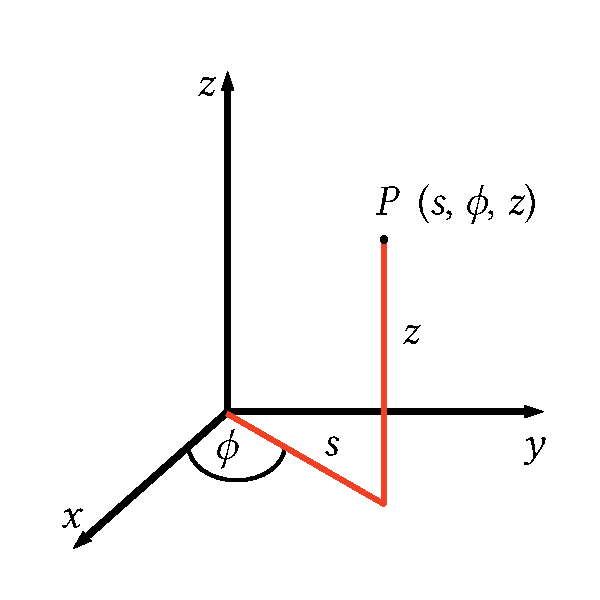
\includegraphics[width=0.5\linewidth]{Figures/Chapter1/fig_cyl_coord}
\caption{Cylindrical coordinates $(s, \phi, z)$.}
\label{fig_cyl_coord}
\end{figure}

So far, I've written everything down in Cartesian coordinates, but we'll use cylindrical coordinates $(s, \phi, z)$ frequently as well.  Figure \ref{fig_cyl_coord} shows the usual cylindrical coordinate setup, and it's clear that
\[
x = s \cos \phi, \quad y = s \sin \phi, \quad \text{and} \quad z = z.
\]
We can write the fluid velocity in cylindrical coordinates as
\begin{equation}
\label{eq_u_cyl}
\vec{u} = u_s(s, \phi, z, t) \, \unit{s} + u_\phi (s, \phi, z, t) \, \unit{\phi} + u_z(s, \phi, z, t) \, \unit{z}.
\end{equation}
I'll avoid using the ``bracket'' shorthand if we're using cylindrical coordinates.

In much of our examination of fluid dynamics, we'll deal with special cases and symmetries which will make our job (slightly) easier.  The below examples discuss two of these special cases.

\begin{example}[Steady Flow]
A \emph{steady flow} has no explicit time dependence, so that
\begin{equation}
\frac{\partial \vec{u}}{\partial t} = 0.
\end{equation}
This means that, at any point, the speed and direction of the flow are constant. We'll be dealing with this case quite frequently, especially at the beginning of the book.
\end{example}

\begin{example}[Two Dimensional Flow]
A \emph{two dimensional} flow has the form
\begin{equation}
\vec{u} = [u(x, y, t), v(x, y, t), 0].
\end{equation}
Note that not only is there no $z$ component to the velocity field, but there is furthermore no $z$ dependence on the
$x$ and $y$ components, either.
\end{example}

%
%
%

\section{Visualizing Fluid Flow}

%
%

\subsection{Vector Plots}

One way to visualize the flow of a fluid is by drawing a vector for $\vec{u}$ at a sample of positions and, if necessary, times.

\begin{example}[Flow about a stagnation point]
\label{ex_stag_point1}
For example, consider the fluid velocity vector field
\begin{equation}
\label{eq_stag}
\vec{u} = [\alpha x, -\alpha y, 0].
\end{equation}
This is an example of two-dimensional steady flow, and represents the flow around a \emph{stagnation point}, which is a point in the fluid which is not flowing.  The vector plot for this flow is given in Figure \ref{fig_vector_plot}. 
\end{example}

\begin{figure}
\centering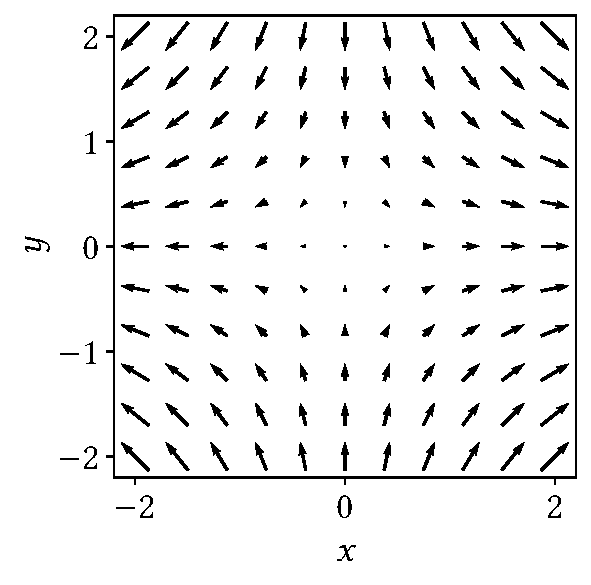
\includegraphics[width=0.5\linewidth]{Figures/Chapter1/fig_vector_plot}
\caption{A vector plot for flow about a stagnation point.  Here the parameter $\alpha = 1$.  Note that at the point $(0,0)$ the flow velocity is zero; that's what makes it a stagnation point. }
\label{fig_vector_plot}
\end{figure}



\subsection{Streamlines}

A more common way to visualize fluids is with \emph{streamlines}.  A streamline is a curve that, at time \(t\), has the same direction as \(\vec{u}(\vec{r}, t)\) at each point. This is a concept you might be familiar with from electrodynamics -- electric field lines are very similar.  Like field lines, streamlines can't cross, since that would imply that a particular fluid element at that point would have two different velocities.  There's one exception to this rule, of course -- streamlines can cross at points in the fluid where the velocity is \emph{zero}.

How do we calculate and plot streamlines? Well, we first parameterize a streamline curve, using $\xi$ as the parameter, as 
\[
x(\xi), \quad y(\xi), \quad z(\xi),
\] 
so that, as $\xi$ changes, the functions $x$, $y$, and $z$ trace out the streamline curve.   From the definition of a streamline, we know that
\[
\frac{dx}{d\xi} = ku, \quad \frac{dy}{d\xi} = kv, \quad \frac{dz}{d\xi} = kw,
\] 
where $k$ is some constant (and different streamlines will have different -- but unique -- values of $k$). Since $k$ is the same along each streamline, we must have
\begin{equation}
\frac{dx/d\xi}{u} = \frac{dy/d\xi}{v} = \frac{dz/d\xi}{w}.
\end{equation} 
This means that, given the functional form of $u$, $v$, and $w$, we can find $x(\xi)$, $y(\xi)$, and $z(\xi)$.

In addition to streamlines, \emph{pathlines} and \emph{streaklines} are sometimes used to visualize and describe fluid flow.  However, for steady flow -- which we'll mostly be dealing with -- they're the same as streamlines, so we won't worry about them too much.  If you're interested, Problem \ref{prob_unsteady} takes a look at an unsteady case where the path lines are different from the streamlines.

%You can watch a nice video about it (as well as some other aspects of visualizing fluids) at \url{https://youtu.be/nuQyKGuXJOs}\footnote{This is just one video in a whole series by the National Committee for Fluid Mechanics Films.  Despite their age, they're great, and I highly recommend watching the ones that are relevant to us.}, and Problem \ref{prob_unsteady} takes a look at an unsteady case where the path lines are different from the streamlines.

\begin{example}[Plotting Streamlines]
\label{ex_stag_stream}
As an example of calculating and then plotting streamlines, let's go back to our flow about a stagnation point, Equation \ref{eq_stag}.  Since this is two dimensional flow, we can ignore $w$ and $z$ dependence and look at 
\[
\frac{dx/d\xi}{u} = \frac{dy/d\xi}{v}.
\]
Plugging in \(u\) and \(v\) for this case, and removing the parameter $\xi$ for simplicity, gives us
\[
\frac{dx}{\alpha x} = -\frac{dy}{\alpha y}.
\] 
Integrating both sides and solving for \(y\) gives the function 
\begin{equation}
y(x) = \frac{c}{x}.
\label{eq_stream_ex}
\end{equation}
That's our answer; \(c\) is the integration constant, which will vary from streamline to streamline.  Figure \ref{fig_streamline_example} shows the streamlines plotted; compare with the vector plot in Figure \ref{fig_vector_plot}.
\end{example}

\begin{figure}[t]
\centering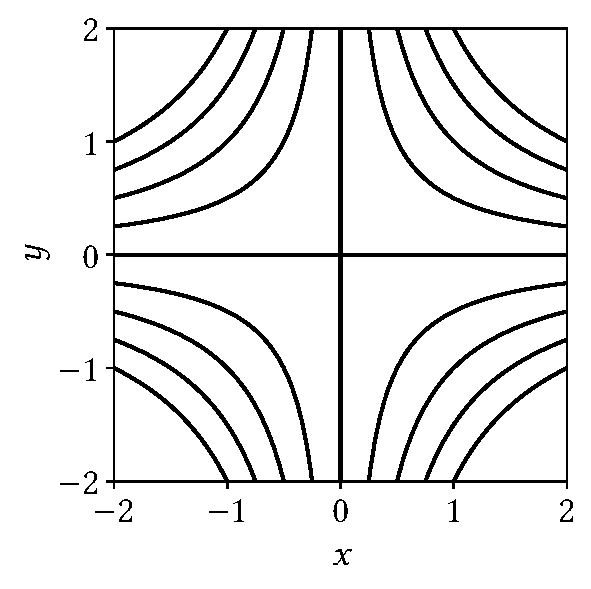
\includegraphics[width=0.5\linewidth]{Figures/Chapter1/fig_streamline_example}
\caption{Streamlines plotted from Equation \ref{eq_stream_ex}, for a variety of values of $c$ ranging from $-2$ to $2$.  Note that the streamlines cross at the stagnation point; that's the only place where they're allowed to.}
\label{fig_streamline_example}
\end{figure}

%
%
%

\section{Total Derivative and Acceleration}
\label{sec_tot_deriv}

Now that we know how to visualize the flow of a fluid, we need to be able to calculate how it \emph{changes}.  

Let $f(x, y, z, t)$ be some quantity of interest -- it might be a component of velocity ($u$ or $v$, say), or maybe the density of the fluid $\rho$, or even the concentration $c$ of a certain pollutant in the fluid.  If we're then looking at one particular (fixed) location -- say, $x, y, z$ -- in the fluid, then $\partial f / \partial t$ gives the rate of change of $f$ at that position.

On the other hand, we might want to know how $f$ changes as we move along with the fluid.  In this case, we might imagine attaching ourselves to a certain \emph{fluid element} -- a small ``blob'' of the fluid -- and measuring how $f$ changes as we move along with it.  This rate of change is given by the so-called \emph{total} or \emph{material} derivative,\footnote{There are many other names for this kind of derivative, too; according to Wolfram MathWorld, it's also called the convective derivative, the advective derivative, derivative following the motion, hydrodynamic derivative, and Lagrangian derivative, among a few others.}
\[
\frac{Df}{Dt} \equiv \frac{df}{dt} = \frac{d}{dt} f[x(t), y(t), z(t), t].
\]
Now, $x(t)$, $y(t)$, and $z(t)$ all change as we move with the flow, and of course
\[
\frac{dx}{dt} = u, \quad \frac{dy}{dt} = v, \quad \text{and} \quad \frac{dz}{dt} = w.
\]
So, applying the chain rule to the derivative above, we get
\begin{align*}
\frac{Df}{Dt} & =  \frac{\partial f}{\partial x}\frac{dx}{dt} + \frac{\partial f}{\partial y}\frac{dy}{dt} + \frac{\partial f}{\partial z}\frac{dz}{dt} + \frac{\partial f}{\partial t} \\
& = u \frac{\partial f}{\partial x} + v \frac{\partial f}{\partial y} + w \frac{\partial f}{\partial z} + \frac{\partial f}{\partial t}.
\end{align*}
This can be written more compactly using vectors:
\begin{equation}
\label{eq_total_deriv}
\boxed{
\frac{Df}{Dt} = \frac{\partial f}{\partial t} + (\vec{u} \cdot \vec{\nabla}) f.
}
\end{equation}
Careful with that dot product; the gradient operator $\vec{\nabla}$ operates on the function $f$, so you can't switch the order.  In this case, $(	\vec{u} \cdot \vec{\nabla}) \neq (\vec{\nabla} \cdot \vec{u})$.

As an example of applying the total derivative, let's take $f$ to be the fluid velocity itself:
\begin{equation}
\label{eq_accel}
\boxed{
\frac{D \vec{u}}{Dt} = \frac{\partial \vec{u}}{\partial t} + (\vec{u} \cdot \vec{\nabla}) \vec{u}.
}
\end{equation}
This, as you might suspect, is the \emph{acceleration} of the fluid element at position $\vec{r}$.

Note that if the material derivative is \emph{zero},
\[
\frac{Df}{Dt} = 0,
\]
that implies that the quantity $f$ doesn't change \emph{for a particular fluid element.}  On the other hand, if just
\[
(\vec{u} \cdot \vec{\nabla}) f = 0,
\]
that means that $f$ will be constant \emph{along a streamline.}  This might not be immediately obvious, so let's prove it.  Let $\unit{e}_s$ be a unit vector that is always parallel to a streamline in the direction of the flow.  Since a streamline is always tangent to the flow, we can write
\[
\vec{u} = |\vec{u}| \, \unit{e}_s,
\]
so that
\[
(\vec{u} \cdot \vec{\nabla}) f = (|\vec{u}| \, \hat{\vec{e}}_s \cdot \vec{\nabla}) f = (|\vec{u}| \frac{\partial }{\partial s} )f = |\vec{u}| \frac{\partial f}{\partial s} = 0.
\]
Thus $\partial f / \partial s = 0$ and the quantity $f$ must be constant along the direction $s$, which is along the streamline.

\begin{example}[Acceleration of the fluid]
Let's return to our flow around a stagnation point.  What is the acceleration of the flow?

Well, clearly $\partial \vec{u} /\partial t = 0$ (the flow is steady), and so
\[
\frac{D \vec{u}}{Dt} = (\vec{u} \cdot \vec{\nabla} ) \vec{u} = \left( u \frac{\partial}{\partial x} + v\frac{\partial}{\partial y} \right) \vec{u}.
\]
At this point is probably easiest to work out each vector component separately:
\[
\frac{D u}{Dt} =  u \frac{\partial u}{\partial x} + v\frac{\partial u}{\partial y}  = \alpha^2 x,
\]
and
\[
\frac{D v}{Dt} =  u \frac{\partial v}{\partial x} + v\frac{\partial v}{\partial y}  = \alpha^2 y.
\]
So the acceleration is
\[
\frac{D \vec{u}}{Dt} = \alpha^2 x \, \unit{x} + \alpha^2 y \, \unit{y} = [\alpha^2 x, \alpha^2 y].
\]

\end{example}

%
%
%

\section{Incompressible and Irrotational Flow}

\subsection{The Incompressibility Condition}
\label{sec_incompressibility}

Except in one notable case -- gas dynamics -- we'll be dealing with fluids that are \emph{incompressible}.  This essentially just means that the density of the fluid is constant under pressure -- you can't compress it  Stated another way, it means that a ``dyed'' blob of fluid can't change in volume as it moves.  Water is a good example of an incompressible fluid, and we'll even treat air as incompressible in some cases.

We need to be able to write down a mathematical statement of incompressibility.  To do this, consider a fixed, closed surface $S$ in the fluid.  By ``fixed,'' I mean that it's fixed in space, so fluid can move into this closed volume $V$ at some places and out at others; if the fluid is incompressible, though, then however much fluid is \emph{entering} the region must equal the amount that is \emph{leaving}.  

\begin{figure}
\centering
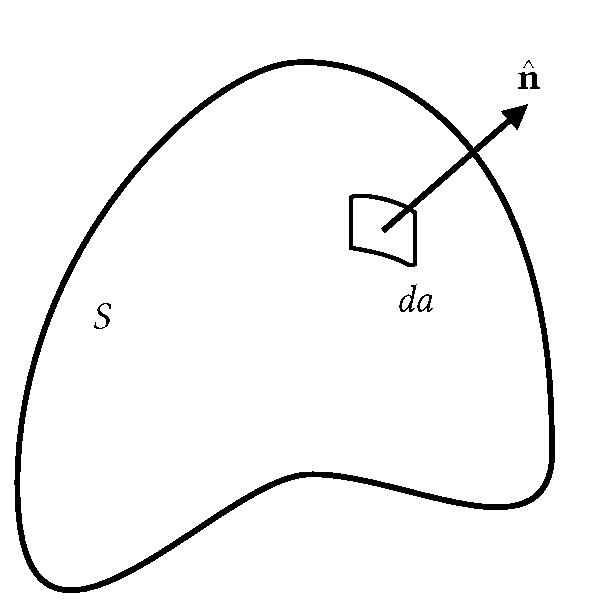
\includegraphics[width=0.5\linewidth]{Figures/Chapter1/fig_closed_surface}
\caption{A fixed, close surface $S$ encolsing a volume $V$.}
\label{fig_closed_surface}
\end{figure}

Consider, then, an infinitesimally small piece of $S$ -- call it $da$ (see Figure \ref{fig_closed_surface}).  The amount of fluid that is leaving $V$ through $da$ is given by
\[
\vec{u} \cdot \unit{n} \, da.
\]
This expression, where $\vec{u}$ is the fluid velocity at the location of $da$ and $\unit{n}$ points normal to the surface $da$ in the outward direction, is a \emph{volume flow rate}.  It measures the volume of fluid that passes through $da$ per unit time.  The dot product ensures we get only that fluid which is moving \emph{through} the tiny surface, whether it's flowing outward (positive dot product) or inward (negative dot product).

To find the total amount of fluid leaving the entire surface $S$, we can just integrate over that surface:
\[
\int_S \vec{u} \cdot \hat{n} \, da
\]
is the net volume rate at which fluid is leaving.  However, for an incompressible fluid, we know this must be \emph{zero}.

To write this in a form a little more usable, we can apply the divergence theorem, which states that
\[
\int_S \vec{F} \cdot \unit{n} \, da = \int_V \vec{\nabla} \cdot \vec{F} \, d\tau.
\]
Here, $\vec{F}$ is some general vector field and $d\tau$ is the infinitesimal volume element.  Our incompressibility condition then becomes
\[
\int_V \vec{\nabla} \cdot \vec{u} \, d\tau = 0.
\]
However, this must be true \emph{anywhere} in the fluid and for any size volume; that means the integrand itself must be zero:
\begin{equation}
\label{eq_incompressibility}
\boxed{
\vec{\nabla} \cdot \vec{u} = 0.
}
\end{equation}
This is the \emph{incompressibility condition}; unless we say otherwise, every flow must obey it.

\begin{example}[Incompressible flow]
\label{ex_stag_point2}
Is our flow about a stagnation point incompressible?  Let's check.  Recall that $\vec{u} = [\alpha x, -\alpha y]$.  The divergence of $\vec{u}$ is then
\[
\vec{\nabla} \cdot \vec{u} = \frac{\partial u}{\partial x} + \frac{\partial v}{\partial y} = \alpha + (-\alpha) = 0,
\]
just as we require.
\end{example}


\subsection{Vorticity}

The \emph{vorticity} of a flow is defined as
\begin{equation}
\boxed{
\vec{\omega} = \vec{\nabla} \times \vec{u}.
}
\end{equation}
For a two dimensional flow $\vec{u} = [u(x, y), v(x, y), 0]$, we can write the vorticity as $\vec{\omega} = [0,0,\omega]$, where
\[
\omega = \frac{\partial v}{\partial x} - \frac{\partial u}{\partial y}
\]
(note the difference between the bolded $\vec{\omega}$ and the non-bold $\omega$ -- one is the full vector, and one is just the magnitude of that vector).

What, exactly, is vorticity?  It's related to the \emph{rotation} of the flow, but is a little trickier than that.  A couple of examples is probably best first.

\begin{example}[Vorticity of shear flow]
The flow given by $\vec{u} = [\beta y, 0, 0]$ is called a \emph{shear flow}; a vector plot is shown in Figure \ref{fig_shear}.  This fluid is clearly \emph{not} rotating, but it does have vorticity.  Since it's two dimensional, we can easily calculate $\omega$:
\[
\omega = \frac{\partial v}{\partial x} - \frac{\partial u}{\partial y} = -\beta.
\]
The vorticity is constant throughout the fluid.
\end{example}

\begin{figure}
\centering
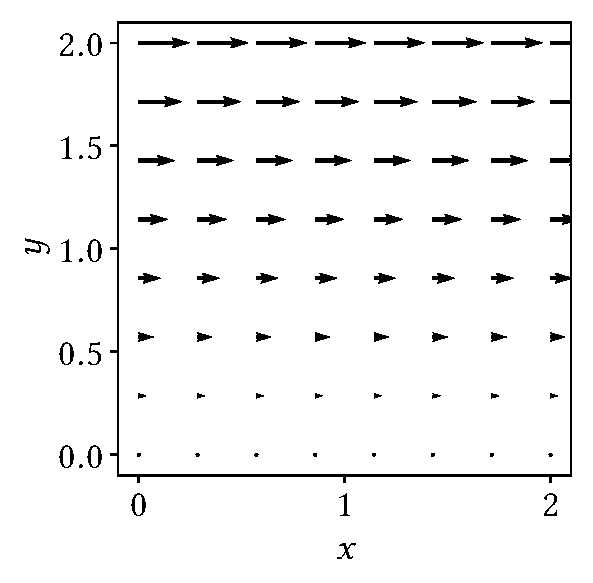
\includegraphics[width=0.5\linewidth]{Figures/Chapter1/fig_shear_vector}
\caption{A shear flow, with $\beta = 1$.}
\label{fig_shear}
\end{figure}

\begin{example}[Vorticity of a line vortex]
\label{ex_vorticity_line_vortex}
Next, let's look at the flow
\begin{equation}
\vec{u} = \frac{k}{s} \, \unit{\phi}.
\end{equation}
This is written in cylindrical coordinates, and the vector plot is shown in Figure \ref{fig_vortex}.  We'll be seeing this kind of flow quite a bit, so make sure you're familiar with it -- but for now all we need to know is that the fluid is clearly rotating.  Despite this, the vorticity is actually zero; I'll let you show this for homework (see Problem \ref{prob_vortex_vorticity}).
\end{example}

\begin{figure}
\centering
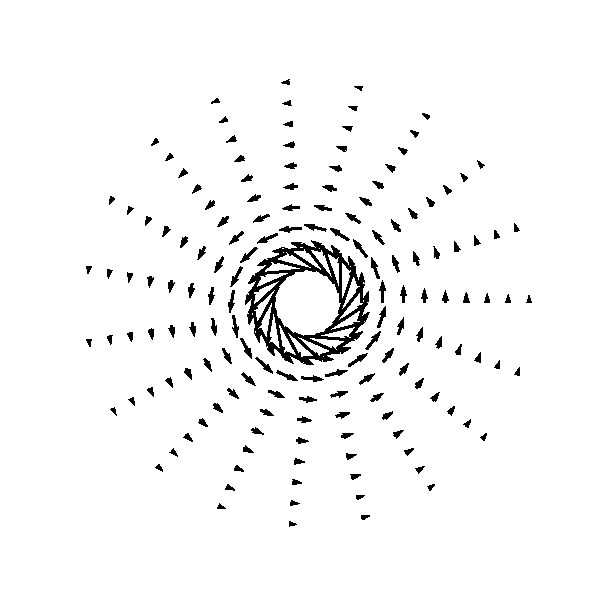
\includegraphics[width=0.5\linewidth]{Figures/Chapter1/fig_line_vortex_vector}
\caption{A line vortex flow, with $k = 1$.}
\label{fig_vortex}
\end{figure}

Despite these examples, vorticity really is related to the rotation of the flow -- but it's the \emph{local} rotation that it measures.  If we built a simple ``vorticity meter,'' using two pieces of plastic and marking one tip so we can see it, the difference between the shear flow and the line vortex flow is very noticeable; see Figure \ref{fig_vorticity1}.  In the shear flow the vorticity meter will itself rotate due to the local rotation of the fluid, while the meter in the line vortex flow will travel in a circlular path but not rotate.

Finally, a bit of terminology: if the vorticity of a flow is zero, we say that it is \emph{irrotational}, so that
\begin{equation}
\boxed{
\vec{\nabla} \times \vec{u} = 0
}
\end{equation}
for an irrotational flow.

\begin{figure}
\centering
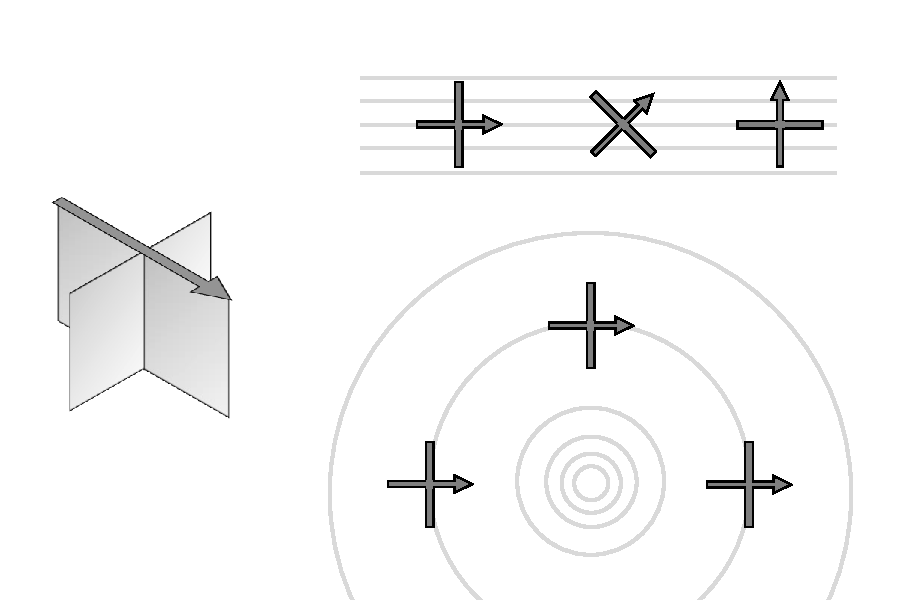
\includegraphics[width=0.7\linewidth]{Figures/Chapter1/fig_vorticity1.pdf}
\caption{A simple vorticity meter shows the difference between two rotating flows -- the shear flow (top) and line vortex flow (bottom); it measures the \emph{local} rotation in a fluid.}
\label{fig_vorticity1}
\end{figure}

%
%
%

\section{Viscosity}
\label{sec_viscosity}

Experiment shows that a fluid doesn't ``slip'' along a boundary; instead, there is a thin boundary layer across which the flow speed drops smoothly and rapidly to zero (see Figure \ref{fig_boundary}).  The fluid elements in contact with the surface therefore move with the surface; this is called the \emph{no-slip condition}.

\begin{figure}
\centering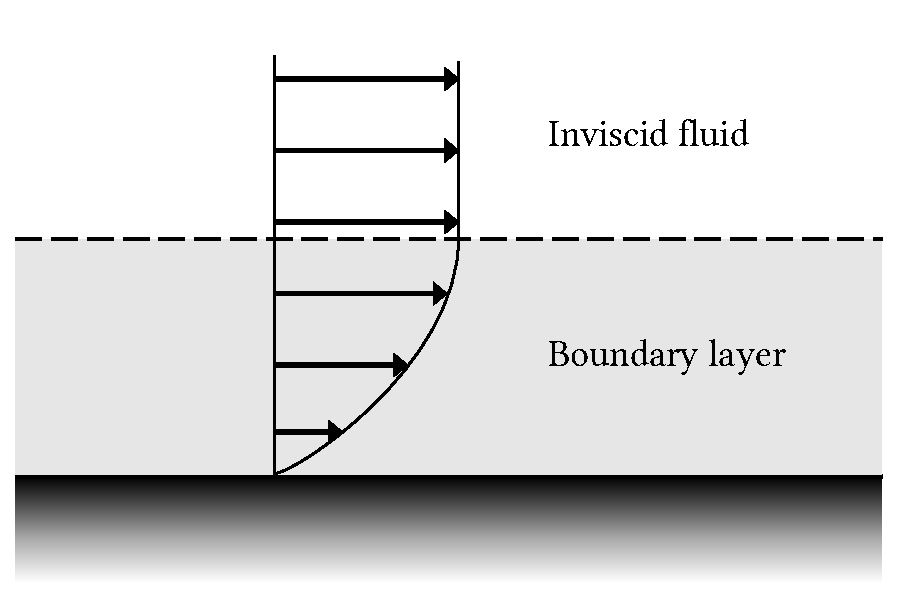
\includegraphics[width=0.7\linewidth]{Figures/Chapter1/fig_boundary_layer}
\caption{The boundary layer in a viscous fluid.  The arrow here represent the fluid velocity in the horizontal direction -- above the boundary layer, we can treat the fluid as inviscid, but within the velocity drops off to zero.}
\label{fig_boundary}
\end{figure}

The boundary layer comes from the viscosity of the fluid, which is defined (for so-called Newtonian fluids) via the tangential stress $\tau$,
\begin{equation}
\label{eq_visc_def}
\tau = \mu \frac{du}{dy}.
\end{equation}
We'll see where this comes from later on, in Section \ref{sec_ns_deriv}; for now, the quantity we want to focus on is the \emph{coefficient of viscosity} $\mu$.

Actually, we'll more frequently use the \emph{kinematic viscosity} $\nu$, defined by
$$
\nu \equiv \frac{\mu}{\rho},
$$
where $\rho$ is the density of the fluid. Some common viscosities (for a temperature of $15^\circ$C) are shown in Table \ref{tab_viscosity}.

\begin{table}[t]
\centering
  \begin{tabular}{l|l}
  & $\nu$ (cm$^2$/s) \\
  \hline \\
  Water & 0.01 \\
  Air & 0.15 \\
  Olive oil & 1.0 \\
  Glycerine & 18 \\
  Golden syrup & 1200
  \end{tabular}
  \caption{The viscosity of some fluids.}
  \label{tab_viscosity}
\end{table}

In some situations, the viscosity of a fluid can be neglected; we'll call the fluid \emph{inviscid} in that case:
\begin{equation}
\boxed{
\nu = 0
}
\end{equation}
for inviscid flow.  Even in situations where the viscosity is very small, though, the presence of the boundary layer can add significant complexity.  Because of the much larger velocity gradient within the boundary layer (where the fluid speed drops to zero  rapidly), the viscous stress becomes significant there, even when $\nu$ is normally small enough that we could neglect viscous effects elsewhere in the flow.

There's an additional feature of boundary layers that make them important dynamically -- in certain situations, they can actually separate from the boundary itself, causing the \emph{entire} flow to be quite different than that predicted by inviscid theory.  This is shown in Figure \ref{fig_boundary_sep} for low-viscosity flow past an aerofoil.  Inviscid theory predicts the flow to the left, but boundary layer separation causes the flow on the right, where a large wake has developed past the aerofoil.

\begin{figure}[t]
\centering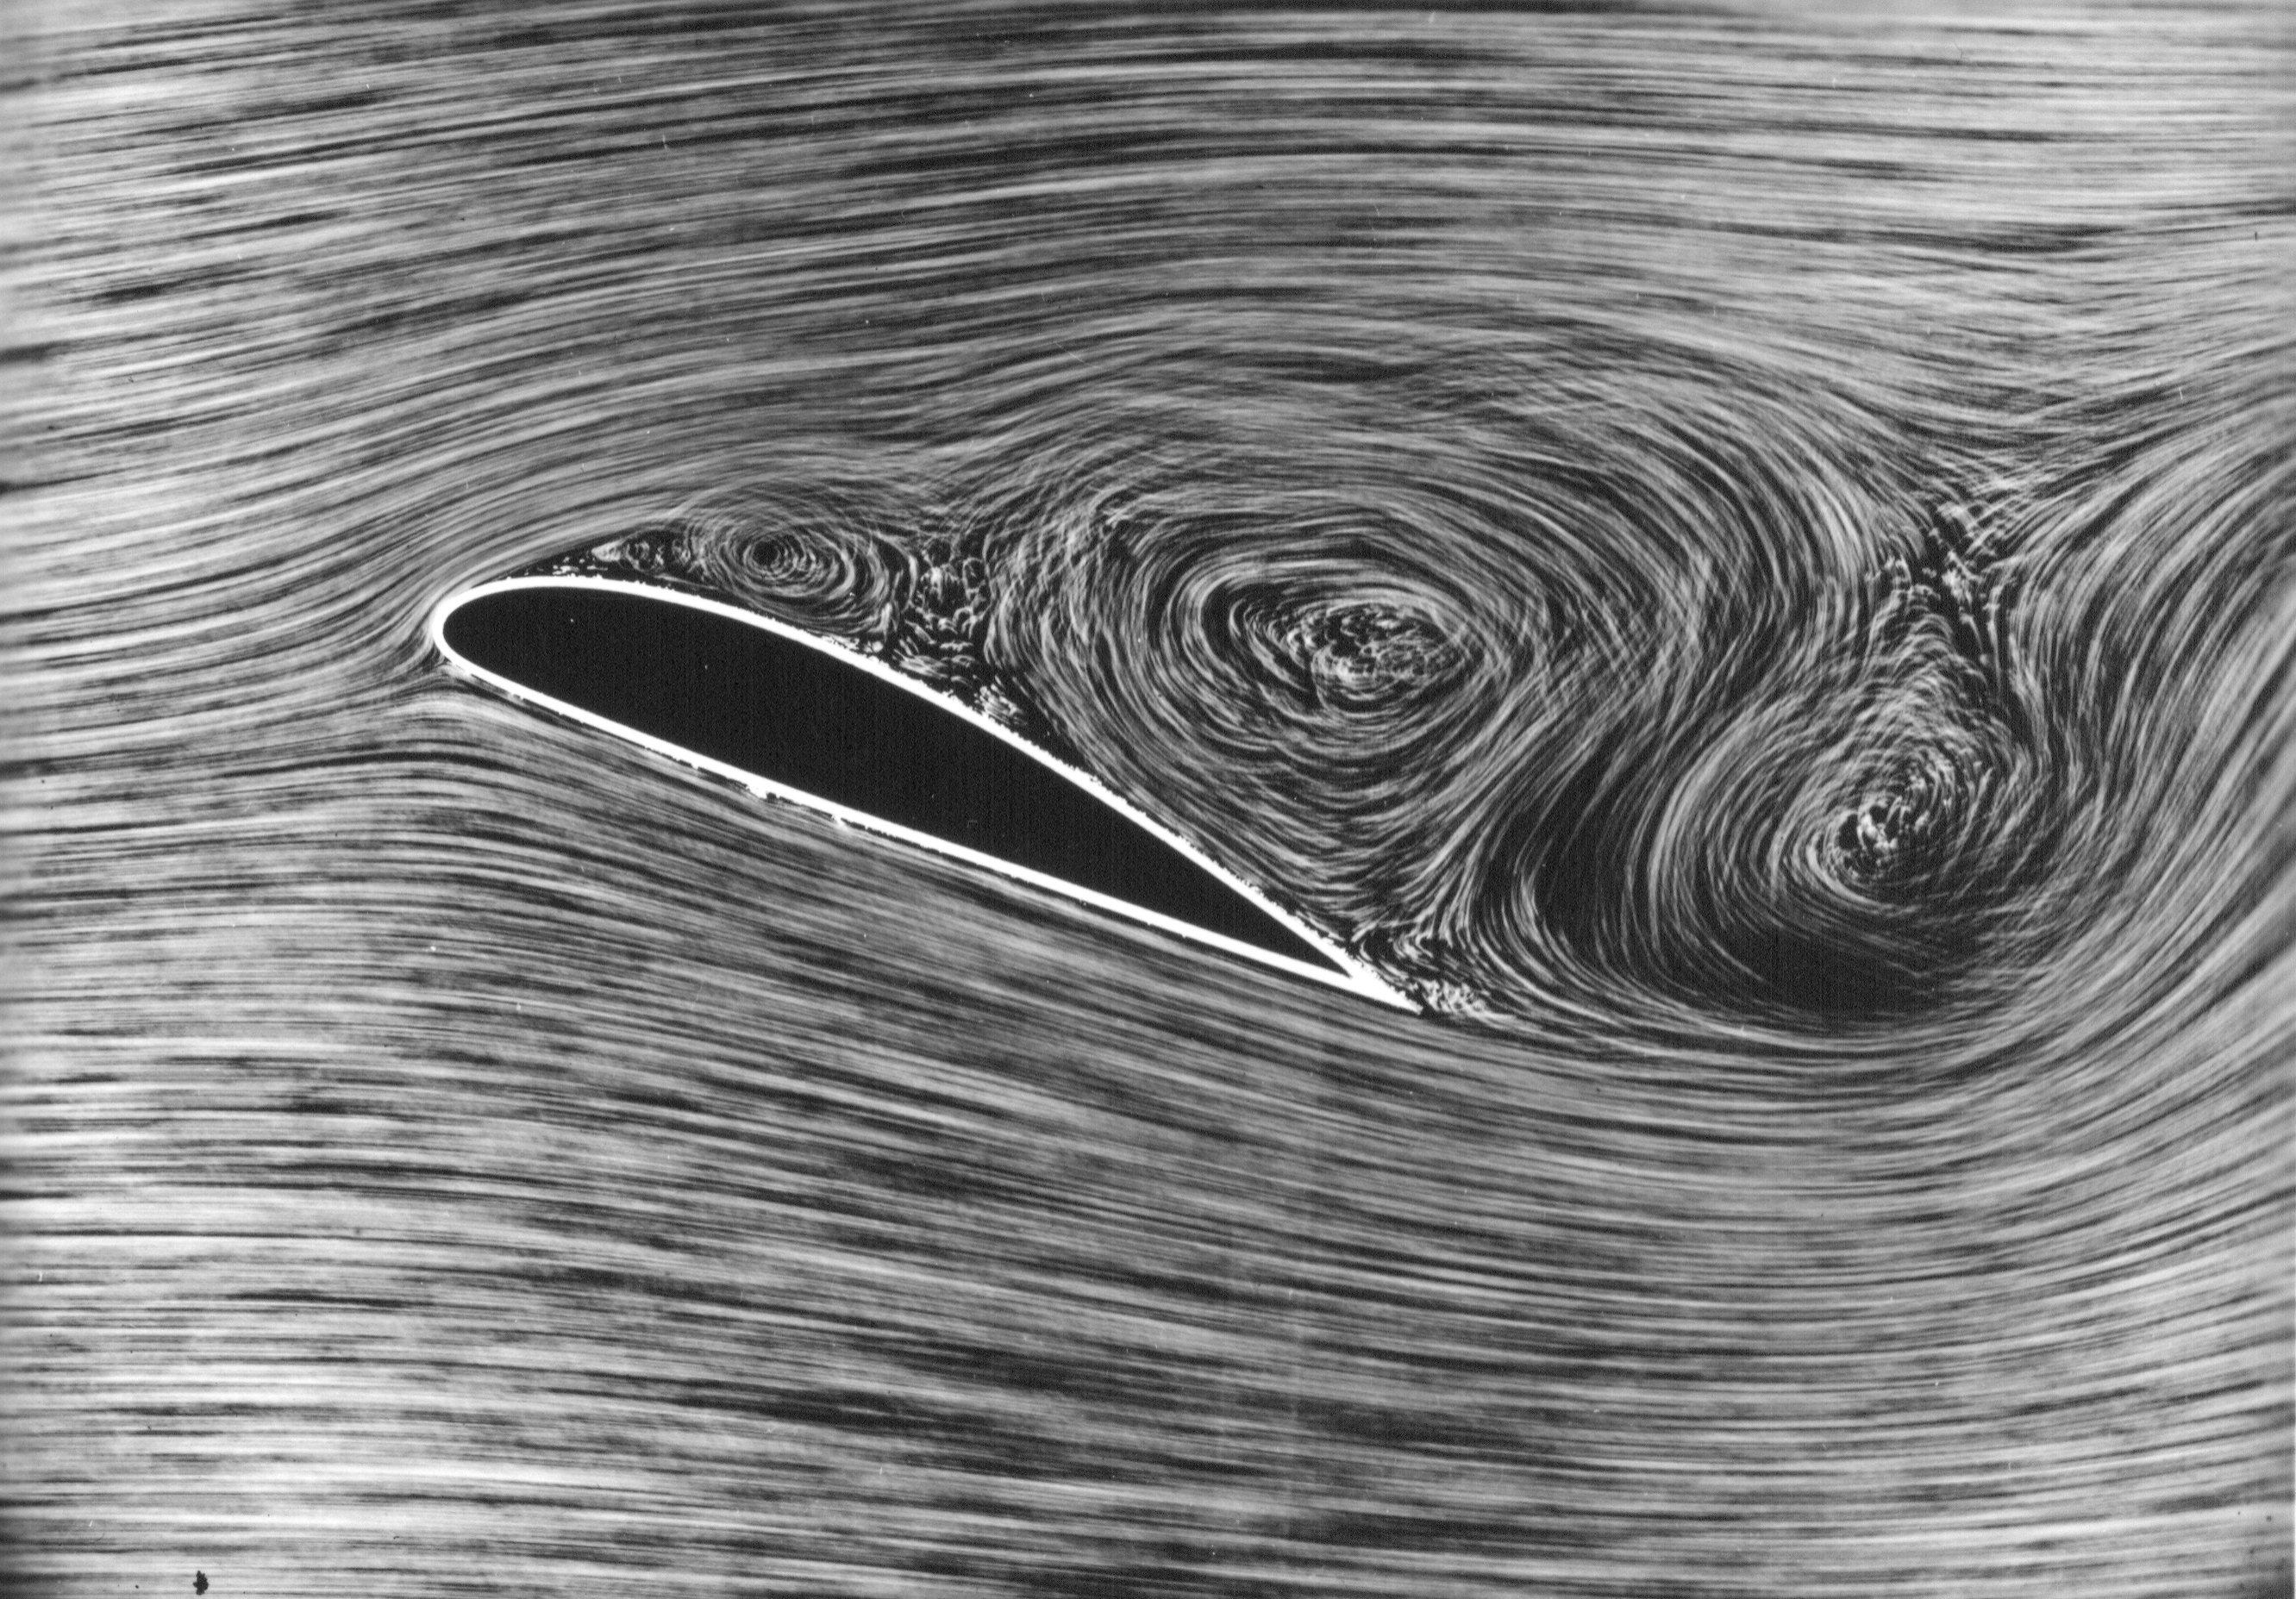
\includegraphics[width=0.7\linewidth]{Figures/Chapter1/fig_boundary_layer_sep.jpg}
\caption{Boundary layer separation occurring in flow past a smooth aerofoil.  (Photo: DLR, CC-BY 3.0)}
\label{fig_boundary_sep}
\end{figure}

One way to characterize how important viscosity is to the flow dynamics is with the \emph{Reynolds number}, defined by
\begin{equation}
R = \frac{UL}{\nu},
\end{equation}
where $U$ and $L$ are velocity and length scales characteristic to the flow (say, for example, the speed of an airplane and the width of its wing).  For large Reynolds number -- greater than a few thousand -- viscosity can be neglected, but the flow can become unstable and \emph{turbulent}.  Below this the flow is smooth, or \emph{laminar}, but viscosity effects can still usually be neglected.  For small Reynolds number, however -- less than one -- viscosity becomes important in how the fluid behaves.



\section*{Problems}
\addcontentsline{toc}{section}{Problems}
\markright{Problems}%

\begin{problem}[Streamlines]
Consider the flow given by 
\[
\vec{u} = [x, x(x-1)(y+1), 0].
\]
Find an equation for the streamlines of the flow and plot them.
\end{problem}

\begin{problem}[ Unsteady flow]
\label{prob_unsteady}
Consider the \emph{unsteady} flow given by
\[
\vec{u} = [U, kt],
\]
where $U$ and $k$ are constants.  Show that the streamlines are straight lines at any particular point in time, and describe their behaviour as time goes on.  Then show that the path a fluid particle follows is parabolic rather than a straight line.  This is an example of how, for unsteady flow, fluid elements do not follow streamlines.

\end{problem}

\begin{problem}[Vector calculus practice]
Calculate the divergence and curl of the following vector fields.  State which flows are incompressible and which are irrotational (or both).

\begin{align*}
\text{(a) } & \vec{u} = [x^2, 3xz^2, -2xz] \\
\text{(b) } & \vec{u} = [xy, 2yz, 3zx] \\
\text{(c) } & \vec{u} = [y^2, 2xy+z^2, 2yz].
\end{align*}

\end{problem}

\begin{problem}[More vector calculus practice]
\label{prob_vc2}
Prove that the curl of a gradient  is always zero and that the divergence of a curl is always zero.

\end{problem}


\begin{problem}[Concentration of a dye]
Consider the flow about a stagnation point,
\[
\vec{u} = [\alpha x, -\alpha y],
\]
where $\alpha$ is a positive constant.  Suppose a coloured dye (food colouring, for example) is introduced into the fluid, and it's concentration is given by
\[
c(x, y, t) = \beta x^2 y e^{-\alpha t},
\]
for $y>0$, and where $\beta$ is a constant.  Does the dye concentration for any particular fluid element change with time?
\end{problem}

\begin{problem}[Acceleration of a rotating fluid]
A fluid in uniform rotation with angular velocity $\Omega$ is given by
\[
\vec{u} = [-\Omega y, \Omega x, 0].
\]
Create a vector plot of the fluid flow, and then calculate the acceleration of the fluid and show that it can be written as
\[
-\Omega^2 \vec{r}.
\]
Is this acceleration what you expect? 
\end{problem}


\begin{problem}[Conservation of mass]
\label{prob_conserve_mass}
If the fluid is compressible, we can derive a condition to replace Equation \ref{eq_incompressibility} by assuming that mass must be conserved.  Use arguments similar to those in Section \ref{sec_incompressibility} to show that it implies
\begin{equation}
\label{eq_continuity}
\boxed{
\frac{\partial \rho}{\partial t} + \vec{\nabla} \cdot (\rho \vec{u} ) = 0.
}
\end{equation}
This is called the \emph{continuity equation}.  Show also that, if the density is constant in space and time, this reduces to the usual incompressibility condition.
\end{problem}


\begin{problem}[Vorticity of a line vortex]
\label{prob_vortex_vorticity}
Show that the vorticity of a line vortex, 
\[
\vec{u} = \frac{k}{s} \unit{\phi},
\]
is zero everywhere except at the origin, where it blows up.
\end{problem}



\begin{problem}[The Reynolds number] Give an order of magnitude estimate of the Reynolds number for

(a) Flow past the wing of a Boeing 737 cruising at 150 m/s.

(b) A thick layer of golden syrup draining off a spoon.

(c) Air flowing through the trachea during normal breathing.

(d) Water flowing through a creek bed.

You'll have to estimate a speed and size for most of these.  Which could be turbulent?  Which would require viscous flow theory, and which inviscid theory?

\end{problem}


\chapter{Viscous Fluids}

%
% --- SECTION - THE NS EQ ---
% 

\section{The Navier-Stokes Equations}

We've discussed a lot of different flows already -- about a stagnation point, a shear flow, a line vortex flow -- but we haven't yet talked about how we \emph{find} the fluid velocity $\vec{u}$.  That is, after all, the whole goal of fluid dynamics!

In short (and we'll come back to this in Section \ref{sec_ns_deriv} for a full derivation), fluid dynamics is governed by the \emph{Navier-Stokes equation},
\begin{equation}
\label{eq_navier_stokes}
\boxed{
\frac{D \vec{u}}{Dt} = -\frac{1}{\rho} \grad p + \nu \nabla^2 \vec{u} +  \vec{g}.
}
\end{equation}
We can recognize some of what's there -- the kinematic viscosity $\nu$ we've already talked about, and the acceleration is the left hand side.  In addition, there's also:
\begin{itemize}
\item The \emph{density} of the fluid, $\rho(\vec{r}, t)$.  If the fluid is incompressible, this is constant in both space and time.
\item The \emph{pressure} of the fluid, $p(\vec{r}, t)$.  This is a scalar function and usually not uniform throughout the fluid.  Pressure is probably familiar to you, but we'll come back to it and properly define it when we derive the Navier-Stokes equations.
\item The gravitational field $\vec{g}$.  Usually -- but not always -- we'll be dealing with fluids at the surface of the Earth, and define our coordinate system so that $\vec{g} = [0,0,-g]$ where $g = 9.8$ m/s$^2$ as usual. 
\end{itemize}

The Navier-Stokes equations, named after Claude-Louis Navier and George Gabriel Stokes who (independently) derived them, are famously difficult to solve -- they're a set of coupled nonlinear second order partial differential equations.  In fact, showing that solutions to the Navier-Stokes equation always exist and are smooth is one of the seven ``Millennium Prize Problems'' from the Clay Mathematics Institute.  We won't be doing anything so difficult here; for some simple situations, the equations are readily solvable, even if they require some thought and a few tricks.

% SUBSECTION - CARTESIAN COORDS

\subsection{Cartesian Coordinates}

We'll begin with flows that are best described by the usual Cartesian coordinates $x$, $y$, and $z$.  In this coordinate system, the Navier-Stokes equations take on the form
\begin{align}
\label{eq_ns_cart1}
\dfdx{u}{t} + u\dfdx{u}{x} + v \dfdx{u}{y} + w \dfdx{u}{z} = -\frac{1}{\rho} \dfdx{p}{x} + \nu \left( \ddfdx{u}{x} + \ddfdx{u}{y} + \ddfdx{u}{z} \right) + g_x, \\
\dfdx{v}{t} + u\dfdx{v}{x} + v \dfdx{v}{y} + w \dfdx{v}{z} = -\frac{1}{\rho} \dfdx{p}{y} + \nu \left( \ddfdx{v}{x} + \ddfdx{v}{y} + \ddfdx{v}{z} \right) + g_y, \\
\dfdx{w}{t} + u\dfdx{w}{x} + v \dfdx{w}{y} + w \dfdx{w}{z} = -\frac{1}{\rho} \dfdx{p}{z} + \nu \left( \ddfdx{w}{x} + \ddfdx{w}{y} + \ddfdx{w}{z} \right) + g_z.
\end{align}

Furthermore, we'll assume our fluids are \emph{incompressible}, so that they must also satisfy the incompressibility condition, Equation \ref{eq_incompressibility}, which in Cartesian coordinates is
\begin{equation}
\label{eq_incomp_cart}
\dfdx{u}{x}  + \dfdx{v}{y} + \dfdx{w}{z} = 0.
\end{equation}

Those are an impressively complicated looking set of equations.  To solve them, we'll first make some assumptions based on the \emph{physical} nature of the problem we're examining; as we'll see in a moment, that will allow us to remove some terms and simplify things considerably.

%
% --- SECTION - SIMPLE VISCOUS FLOWS ---
% 

\section{Simple Viscous Flows}


% SUBSECTION - STEADY POISEUILLE FLOW

\subsection{Poiseuille Flow in One Dimension}
\label{sec_poise_1d}

Consider fluid flowing steadily between two rigid boundaries, one at $y=0$ and one at $y = h$, under a constant pressure gradient 
\[
\frac{dp}{dx} = -P.
\]
Figure \ref{fig_poise_setup} shows the set-up and our coordinate system.

\begin{figure}
\centering
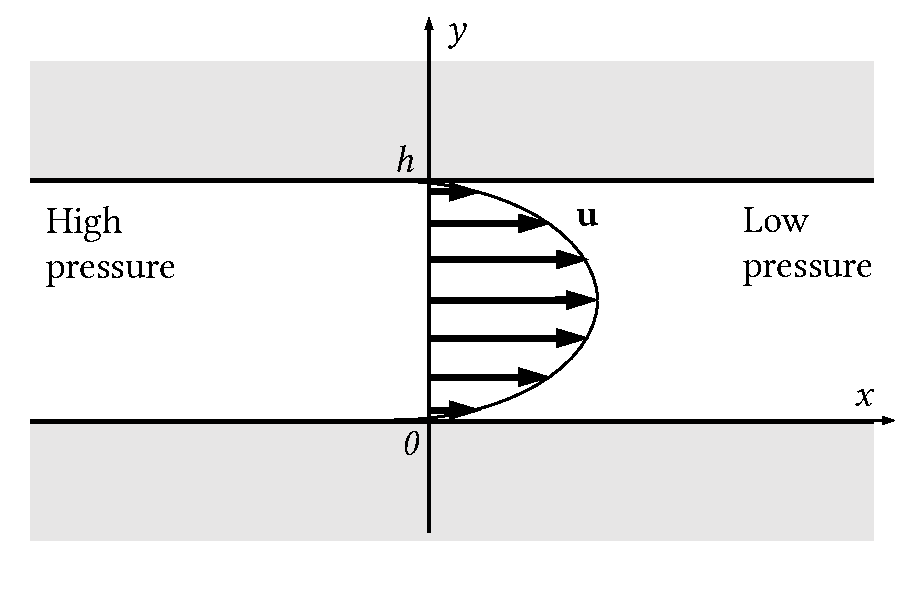
\includegraphics[width=0.7\linewidth]{Figures/Chapter2/fig_poise_setup}
\caption{The fluid will flow to the right due to the pressure gradient.}
\label{fig_poise_setup}
\end{figure}

This problem was first examined by Jean L\'eonard Marie Poiseuille, a physiologist interested in the flow of blood though capillaries and veins,\footnote{Actually, Poiseuille studied a slightly different problem -- see Problem \ref{prob_poise_cyl}.} although it also serves well as a model for air flowing through alveoli in lungs and fluid flowing through a straw.  It's also a great introduction to solving the Navier-Stokes equations, since it's essentially a one dimensional problem, as we'll see.  You can do the slightly more complicated two dimensional problem for homework (Problem \ref{prob_poise_2d}).

The first step to solving the Navier-Stokes equations is to examine symmetries and dependencies.  For example, this is clearly a two dimensional flow, with no dependence on $z$ or flow in the $w$ direction.  This assumes the ``walls'' at $y=0$ and $y=h$ are infinite in extent along the $z$-direction, but that's okay -- it still makes this problem a good approximation in more realistic (finite) situations.  This is also explicitly \emph{steady} flow, so there's no time dependence at all.  All this suggests we can write our the fluid velocity $\vec{u}$ in terms of $x$ and $y$ only:
\[
\vec{u} = [ u(x, y), v(x, y), 0].
\]

Furthermore, since the walls are also infinite in extent along the $x$-direction, we shouldn't expect any $x$-dependence in $\vec{u}$.  If this seems surprising, consider moving our origin in Figure \ref{fig_poise_setup} left or right -- since the pressure gradient is \emph{constant}, exactly where we put the origin along the $x$-direction won't change the velocity at all.  So that means our flow dependence is now
\[
\vec{u} = [u(y), v(y), 0].
\]
That's pretty simple, but we can do even better by looking at the incompressibility condition.  In our flow, $\partial u /\partial x = 0$ since the flow only depends on $y$, so equation (\ref{eq_incomp_cart}) becomes
\[
\dfdx{v}{y} = 0.
\]
That means that $v$ is a constant.  But remember the no-slip condition from Section \ref{sec_viscosity} -- the walls are stationary, so the fluid in contact with them can't be moving either.  Since the velocity is zero at $y=0$ and $y=h$, and $v$ is constant throughout the fluid, $v=0$ everywhere.

That last argument is a little tricky, but one we'll use quite a bit so go over again to make sure you get it.  The result, at the end of the day, is that for this situation, our flow takes on the simple form
\begin{equation}
\vec{u} = [u(y), 0, 0].
\end{equation}
This is called steady \emph{plane-parallel shear flow} -- notice that the flow is in the $x$ direciton but the dependence is along $y$.  Although we derived this form specific to the situation shown in Figure \ref{fig_poise_setup}, it's applicable to others as well -- as long as the flow is two-dimensional, steady, and has that translational symmetry along the $x$-direction.

Now that we know exactly what variables the flow depends on, the Navier-Stokes equations get much simpler to write out (and solve!).  You should convince yourself that the $x$ component, Equation \ref{eq_ns_cart1}, becomes
\begin{equation}
\label{eq_poise_diffeq}
0 = -\frac{1}{\rho} \dfdx{p}{x} + \nu \ddfdx{u}{y}.
\end{equation}
Notice there's no gravity term here; I set $g_x = 0$. In fact, for simplicity I'll assume there is no gravity at all in this problem, so $g_y = g_z = 0$, too.  In Problem \ref{prob_poise_grav} you can see what effect gravity has on the situation, but it won't change the nature of it very much.  The other two Navier-Stokes equations just say that the pressure doesn't depend on $y$ or $z$, but we're already told that there is a constant pressure gradient in the $x$-direction, so that's nothing new.

Solving the differential equation in (\ref{eq_poise_diffeq}) is straightforward.  Let's write $dp/dx = -P$ and rearrange to get
\[
\frac{d^2u}{dy^2} = -\frac{P}{\nu \rho}.
\]
This is a second order ordinary differential equation which can be solved with two integrations to get
\[
u(y) = -\frac{P}{2\nu \rho} y^2 + c_1 y + c_2,
\]
where $c_1$ and $c_2$ are the two integration constants.

As usual, we can find the constants by applying our \emph{boundary conditions}.  In this case, we need the fluid at the boundary to have the same velocity as the boundary -- that's the no-slip condition again.  So, at the walls, we need
\[
u(0) = 0 \quad \text{and} \quad u(h) = 0.
\]
It follows from this that $c_2 = 0$ and
\[
c_1 = \frac{Ph}{2\nu \rho},
\]
and our final solution is
\begin{equation}
\label{eq_poise_steady}
u(y) = \frac{P}{2\nu \rho} (hy - y^2).
\end{equation}
The velocity profile is a parabola. 

How do we visualize this flow? Streamlines won't be any good here, since the flow is entirely in the $x$-direction -- the streamlines will just be horizontal.  Instead, we can plot the parabola directly on the system as shown in  Figure \ref{fig_poise_setup}, where I've also drawn in some representative vectors for the velocity $\vec{u}$.  In this way we can see at a glance that the flow is strongest in the middle of the walls, and drops to zero at them according to the no-slip condition.



% SUBSECTION - Time Dependent Flow

\subsection{Time Dependent Flow}
\label{sec_poise_time}

The Poiseuille problem we just did is a great first example of solving the Navier-Stokes equations, but it's also an example of \emph{steady flow} -- nothing really changes in time. There are a few ways we can adapt this problem to introduce time dependence; we'll do two here, and you can do another one on your own if you like (Problem \ref{prob_poise_time}).

To add the time-dependence here we'll suppose that the steady flow we found in Section \ref{sec_poise_1d} has been going on for awhile, and at $t=0$ the pressure gradient stops suddenly:
\[
P = - \frac{dp}{dx} = 0 \quad \text{for} \quad t>0.
\]
What happens to the fluid for $t>0$?  Well, presumably it will slowly come to rest; how long does it take, and what does the flow look like until then?  To answer, we'll set up the problem the same way as above (Figure \ref{fig_poise_setup} again), with the boundaries at $y=0$ and $y=h$.  This is still a plane parallel shear problem, but now that we have time-dependence, the Navier-Stokes equation becomes a partial difference equation,
\begin{equation}
\label{eq_poise_pde}
\dfdx{u}{t} = \nu \ddfdx{u}{y}.
\end{equation}

Our boundary conditions are the same as before -- that $u = 0$ at the walls -- but the initial condition is our steady solution, equation (\ref{eq_poise_steady}),
\begin{equation}
\label{eq_poise_ic}
u(y, t=0) = \frac{P}{2\nu \rho} (hy - y^2).
\end{equation}

To solve this partial differential equation, we'll use a tried and true method all physicists should know:  \emph{separation of variables}.  I'll assume here you're a little bit familiar with this technique,\footnote{If not, Griffiths' \emph{Introduction to Electrodynamics} is a great place to look; he has a whole section (3.3 in the third edition) devoted to it.} but I'll still go into enough detail to jog your memory.

To begin, we suppose that the solution, $u(y, t)$, can be written as the product of two single-variable functions:
\begin{equation}
u(y, t) = Y(y) T(t).
\end{equation}
If we plug this directly into Equation \ref{eq_poise_pde} -- noting that the partial derivatives treat one of the functions as a constant and act as an ordinary derivative on the other -- we get
\[
Y \frac{dT}{dt} = \nu T \frac{d^2Y}{dy^2}.
\]
We can rearrange this a bit to get this into a form where all the dependence on time is on the left hand side, and all the $y$-dependence is on the right:
\[
\frac{1}{\nu T} \frac{dT}{dt} = \frac{1}{Y} \frac{d^2Y}{dy^2}.
\]
The magic of separation of variables can now happen:  since $t$ and $y$ are independent variables -- you can change one without changing the other -- both sides of this equation must be constant!  If that weren't the case, we could change $t$ by a small amount, changing the left hand side, but leaving the right hand side the same -- and the two sides would no longer be equal.

Let's call the constant both sides are equal to $-k^2$; we'll see why it's negative in a moment, and why having it squared is a good idea.  In that case, separation of variables has turned our original partial differential equation into two ordinary differential equations:
\begin{align}
\frac{dT}{dt} & = -k^2 \nu T \\
\label{eq_poise_sho} 
\frac{d^2Y}{dy^2} & = -k^2 Y.
\end{align}

The first of these equations is easy to solve; rearrange to get
\[
\frac{dT}{T} = -k^2 \nu dt
\]
and integrate.  With a bit of work, we can write the solution as
\begin{equation}
T(t) = C e^{-k^2 \nu t},
\end{equation}
where $C$ is the integration constant.  We're not quite done with this yet -- we still don't know the value of $C$, or $k$ for that matter -- but let's move on to the second equation.  

Equation (\ref{eq_poise_sho}) one should look familiar,\footnote{If it doesn't, time to brush up on some of your mathematics -- having some familiarity with differential equations is necessary to be successful in learning fluid dynamics.} and it has the general solution
\[
Y(y) = A \sin (ky) + B \cos (ky).
\]
We can apply our boundary condition to this solution right away.  First, we need the fluid to be at rest along the bottom boundary at $y=0$; for that, we'll require $Y(0) = 0$.  If we evaluate the solution at $y=0$, we get $Y(0) = B$, meaning $B$ must be zero.  Our solution therefore becomes
\[
Y(y) = A \sin (ky).
\]
The second boundary condition is a little trickier.  Let's evaluate our solution at $y = h$:
\[
Y(h) = A \sin(kh).
\]
Somehow, this must equal zero as well.  One possibility is to make $A = 0$ -- but then $u = 0$, which doesn't make sense.  Same thing with setting $k = 0$.  But if we set 
\[
kh = n\pi, \quad n = 1, 2, 3, \dots,
\]
then that will work, since the zeros of the sine function are every integer multiple of $\pi$.

This almost completes our full solution; combining $Y(y)$ with $T(t)$ to make the velocity, we get
\[
u(y, t) = Y(y)T(t) = A \sin (n\pi y / h) \, e^{-n^2 \pi^2 \nu t / h^2},
\]
where I've grouped both constants into $A$.  But wait!  This is actually an \emph{infinite} number of solutions, since $n$ is any integrer.  In fact, we can write down the \emph{general} solution to our original partial differential equation as a superposition of all of these individual solutions,
\begin{equation}
\label{eq_poise_sol}
u(y, t) = \sum_{n=1}^\infty A_n \sin(n \pi y / h) \, e^{-n^2 \pi^2 \nu t / h^2}.
\end{equation}
Note that the constant $A$ could be different in each term in the sum, so it has an index $n$ on it.

All we have left to do is find the values of the $A_n$s, which we do by using the initial condition.  In fact, our solution can fit \emph{any} initial condition we want; that's part of the magic of separation of variables.  If we evaluate equation (\ref{eq_poise_sol}) at $t=0$ and equate it to our initial conditions, equation (\ref{eq_poise_ic}), we get
\[
\sum_{n=1}^\infty A_n \sin(n \pi y / h) =  \frac{P}{2\nu \rho} (hy - y^2).
\]
Somehow we have to solve this equation for $A_n$.  We can do that by application of what is sometimes called \emph{Fourier's trick}:\footnote{In fact, you might recognize these techniques as a part of the general theory of Fourier series.} we'll multiply both sides by $\sin(m \pi y/h)$ and integrate from $y=0$ to $y=h$, giving
\begin{equation}
\label{eq_poise_coeff}
\sum_{n=1}^\infty A_n \int_0^h \sin(m\pi y/h) \, \sin(n \pi y / h) \, dy =  \frac{P}{2\nu \rho} \int_0^h (hy - y^2)\sin(m\pi y/h) \, dy.
\end{equation}

Now, the left hand side turns out to be \emph{zero} if $n \neq m$; the two sine functions are called \emph{orthogonal} in that case.  In the case where $n=m$, the integral reduces to
\[
\int_0^h \sin^2(m \pi y / h) \, dy = \frac{h}{2}.
\]
We can combine these two results into one, using the Kronecker delta,
\begin{equation}
\delta_{mn} = \begin{cases} 0 \quad \text{if } m \neq n, \\ 1 \quad \text{if } m = n. \end{cases}
\end{equation}
Thus the left hand side of equation (\ref{eq_poise_coeff}) becomes
\[
\sum_{n=1}^\infty A_n \int_0^h \sin(m\pi y/h) \, \sin(n \pi y / h) \, dy = \frac{h}{2} \sum_{n=1}^\infty A_n  \delta_{mn}.
\]
But the Kronecker delta will \emph{collapse} the sum -- every term in it will be zero except the $m$th one, so we get
\[
\frac{h}{2} \sum_{n=1}^\infty A_n  \delta_{mn} = \frac{h}{2} A_m.
\]

Phew!  That takes care of the left hand side, but we still have to do the right side.  That's a bit messy, since 
\[
\int_0^h (hy - y^2) \sin(m\pi y / h)\, dy = \frac{2h^3}{\pi^3 m^3} \left( 1 - \cos(m\pi) \right).
\]
Why messy?  Because the cosine evaluates to either $+1$ (if $m$ is even, and we get zero) or $-1$ (if $m$ is odd, and we get $2$).  That means we have to handle both of those cases separately.  Putting both sides of equation (\ref{eq_poise_coeff}) together and solving for $A_m$ gives
\begin{equation}
A_m = \begin{cases}
       0, \quad & m \text{ even}, \\
       {4Ph^2}/{\pi^3 \nu \rho m^3}, \quad & m \text{ odd}.
\end{cases}
\end{equation}

Finally, we can write down our full solution to this problem.  Inserting this expression for $A_m$ into equation (\ref{eq_poise_sol}) gives us
\begin{equation}
\label{eq_poise_time_sol}
u(y, t) = \frac{4Ph^2}{\pi^3 \nu \rho} \sum_{n=1, 3, 5 \dots}^\infty \frac{1}{n^3} \sin(n \pi y / h) \, e^{-n^2 \pi^2 \nu t / h^2}.
\end{equation}
That's not particularly nice looking answer, and it took us some work to get there, but we're done.  This gives us the fluid velocity at any time $t$ between the walls.

To take a look at the velocity, let's plot it up at a few times $t$, using the same convention we used in Figure \ref{fig_poise_setup}, where the distance along the $y$-direction is on the vertical axis, and the fluid velocity is along the horizontal.  Figure \ref{fig_poise_time} shows the flow at three times, one of which is $t=0$.  It's clear that, over time, the velocity does in fact go to zero.  If we want to estimate the length of time it takes to come to rest, we can look just at the $n=1$ term in the solution -- it's the dominant term, since each term after it gets smaller by a factor of $1/n^3$.  In that case, we can write the time factor as
\[
e^{-\pi^2 \nu t/h^2} = e^{-t/\tau},
\]
where $\tau = h^2/\pi^2 \nu$ is the characteristic time.  Thus the speed in the channel slows to about 37\% of its initial amount in a time $\tau$.  By a few characteristic times the fluid is practically at rest.

\begin{figure}
\centering
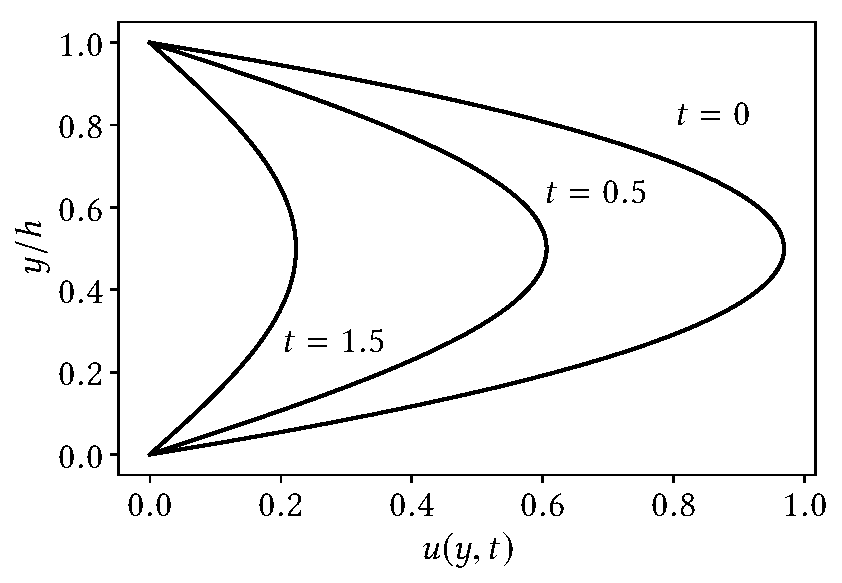
\includegraphics[width=0.7\linewidth]{Figures/Chapter2/fig_poise_time}
\caption{Poiseuille flow is slowing down over time once the pressure gradient shuts off. The velocity is in units of $4Ph^2 /\pi^3 \nu \rho$, and the time is in units of the characteristic time  $\tau = h^2 / \pi^2 \nu$. This plot used about 15 terms in the sum in Equation \ref{eq_poise_time_sol}.}
\label{fig_poise_time}
\end{figure}

% SUBSECTION - IMPULSIVE POISEUILLE FLOW

\subsection{An Impulsively Moved Boundary}
\label{sec_imp}

I'd like to do one more example with the two rigid boundaries before moving on -- mostly because in this example there's an interesting twist with how we'll have to solve the partial differential equation.


This time, we'll start with the fluid at rest in between the two boundaries; the set up is the same as in the above examples and  once again Figure \ref{fig_poise_setup} shows the coordinate system.  In this case, though, there won't be any pressure gradient -- we'll take $dp/dx = 0$ for the whole problem.  Once again, since nothing changes physically about the problem, we have a fluid dependent only on $y$ and flowing only in the $x$-direction, so this is still plane-parallel shear flow.  

We'll put the fluid in motion by, at $t = 0$,  suddenly \emph{jerking} the bottom boundary (the one at $y=0$)  -- we'll pull it to the right with constant speed $U$.  There won't be a period of acceleration here -- it's \emph{impulsively} moved and goes from at rest to moving instantaneously.  Thanks to the no-slip theorem, the bottom boundary will pull on the fluid elements in contact with it, which will in turn exert viscous forces on the fluid above, and so on.  To find out how the fluid responds to the impulsively moved boundary, we'll need to once again solve the Navier-Stokes equation.

It's identical, though, to the above time-dependent problem, equation (\ref{eq_poise_pde}),
\begin{equation}
\label{eq_imp_diffeq}
\dfdx{u}{t} = \nu \ddfdx{u}{y}.
\end{equation}
The initial condition, however, is that the fluid starts at rest,
\begin{equation}
u(y, 0) = 0.
\end{equation}
The boundary conditions come from the no-slip condition, with the top boundary at rest but the bottom moving at constant velocity:
\begin{align}
u(0, t) & = U \quad \text{for } t>0, \\
u(h, t) & = 0.
\end{align}

To solve the differential equation (\ref{eq_imp_diffeq}), we'll once gain use technique of separation of variables.  However, there's a problem in this case -- the boundary condition is nonhomogeneous (since $u(0,t)$ is non-zero).  Unfortunately, separation of variables breaks down with nonhomogeneous boundary conditions (go ahead and try it on your own!).  

We can fix up the problem to deal with that, though, using a standard technique.  First, let's imagine that the flow is actually \emph{steady} -- there's no time dependence.  In that case, our equation simply becomes
\[
\frac{d^2 u_\text{steady}}{dy^2} = 0,
\]
which has the solution
\[
u_\text{steady}(y) = c_1 + c_2 y.
\]
To fit the boundary conditions, we need $c_1 = U$ and $c_2 = -U/h$, so we have
\[
u_\text{steady}(y) = U \left( 1 - \frac{y}{h} \right).
\]
This flow satisfies the differential equation and the boundary conditions, but not the initial conditions -- there's no time dependence at all.  However, it might be reasonable to think that, after a long time has passed, the flow will eventually reach a steady state like this.  In that case, it makes sense to write the \emph{full} solution as
\[
u(y, t) = u_\text{steady}(y) + u_1(y, t),
\]
where $u_1(y, t)$ is an unknown ``transient'' function; clearly, we want $u_1 \to 0$ as $t \to \infty$ so that we get our long-time steady state. 

If we plug this form of $u(y,t)$ into Equation \ref{eq_imp_diffeq}, our differential equation becomes
\begin{equation}
\dfdx{u_1}{t} = \nu \ddfdx{u_1}{y}.
\end{equation}
Notice that $u_\text{steady}$ has disappeared from the differential equation, and it looks like we've just swapped out $u$ for $u_1$.  What have gained?  Well, $u_1$ has different boundary conditions than $u$ -- notably, it now goes to zero at both $y=h$ \emph{and} $y=0$, where the steady state solution cancels the original condition -- and our boundary conditions are now homogeneous:
\begin{align}
u_1(0, t) & = 0 \quad \text{for } t>0, \\
u_1(h, t) & = 0.
\end{align}
The initial condition has also changed, since we need to cancel off the steady state term there, too:
\begin{equation}
\label{eq_poise_imp_ic}
u_1(y, 0) = -u_\text{steady} = -U \left( 1 - \frac{y}{h} \right).
\end{equation}

Now we're ready to solve by separation of variables.  The process and most of the steps are identical to what we just went over in Section \ref{sec_poise_time}, so I'll skip some of the details.  Thanks to the same differential equation and boundary conditions for $u_1$, the solution is once again
\[
u_1(y, t) = \sum_{n=1}^\infty A_n \sin(n \pi y / h) \, e^{-n^2 \pi^2 \nu t / h^2}.
\]
All that's left is to find the $A_n$s that fit the initial conditions, equation (\ref{eq_poise_imp_ic}).  Using Fourier's trick again (multiplying by $\sin(m \pi y / h)$ and integrating) leads to 
\[
A_n = -\frac{2U}{n\pi}.
\]
Finally, adding in the steady-state solution to get $u(y, t)$, we have
\[
u(y, t) = U \left[ 1 - \frac{y}{h} - \frac{2}{\pi} \sum_{n=1}^\infty \frac{1}{n} \sin(n \pi y / h) \, e^{-n^2 \pi^2 \nu t / h^2} \right].
\]

Figure \ref{fig_poise_imp} shows the fluid velocity $u(y,t)$ at a couple of different times.  The characteristic time is the same as in the previous problem; after a few $\tau = h^2/\pi^2 \nu$, the fluid reaches its steady state.


\begin{figure}
\centering
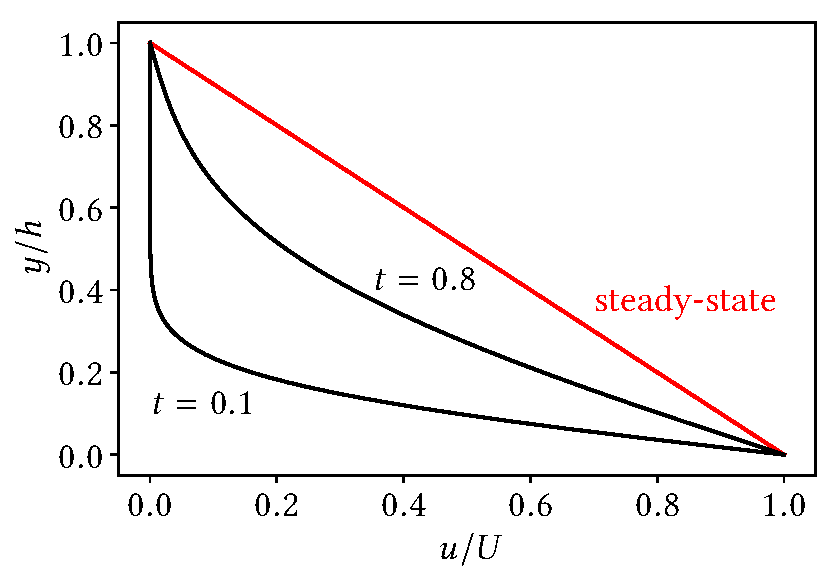
\includegraphics[width=0.7\linewidth]{Figures/Chapter2/fig_poise_imp}
\caption{A boundary suddenly jerked into motion will eventually move the fluid into a steady state.  The time is in units of the characteristic time $\tau$.}
\label{fig_poise_imp}
\end{figure}



% SUBSECTION - ONE BOUNDARY - SELF SIMILAR

\subsection{Self-Similar Flows}
\label{sec_self_similar}

The techniques we used to solve the three previous problems -- integrating an ordinary differential equation, using separation of variables to solve a partial differential equation, and then doing the same thing but with the added twist of using a steady state solution to handle nonhomogeneous boundary conditions -- are all standard techniques physicists use to solve differential equations.  All three problems also had very similar set-ups -- two boundaries and plane parallel shear flow.

I'd like to do one last example of time-dependent plane parallel shear flow before moving on to other kinds of situations, but this time I'll remove the boundary at $y=h$ -- we only have one boundary in this new problem, and it's along the $x$-axis.  Fluid exists only in the region $y>0$, but it can extend up to infinity -- see Figure \ref{fig_self_sim_setup}.

\begin{figure}
\centering
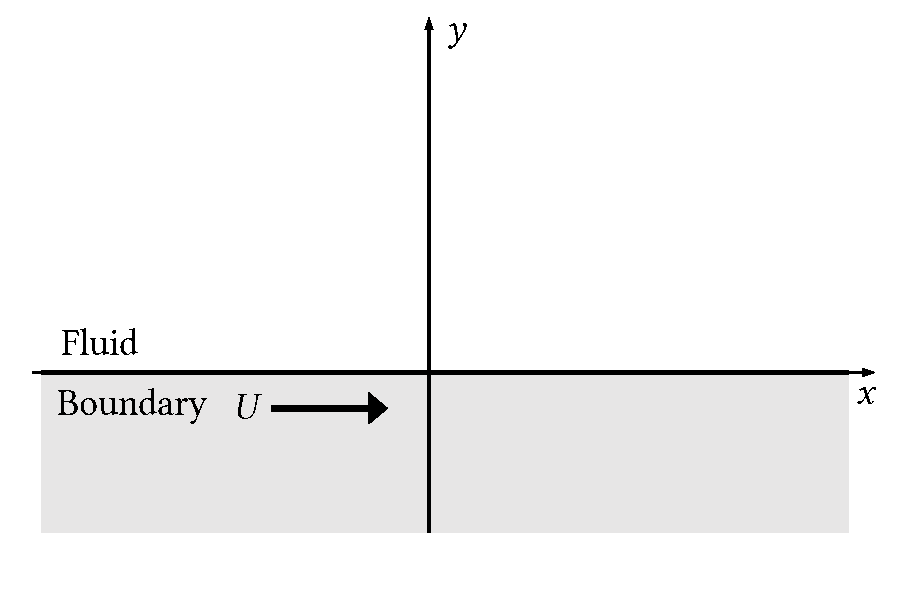
\includegraphics[width=0.7\linewidth]{Figures/Chapter2/fig_self_sim_setup}
\caption{A single boundary is suddenly jerked into motion.  This problem is \emph{self-similar} because it doesn't have a scale.}
\label{fig_self_sim_setup}
\end{figure}

As with the previous example, this boundary will be impulsively put into motion at $t=0$ with a velocity (to the right) of $U$.  We've already gone through the arguments in the last section about what kind of flow this is, and they all hold here, too -- the only difference is in the boundary conditions.  That means we once again have the partial differential equation
\begin{equation}
\label{eq_ss_diffeq}
\dfdx{u}{t} = \nu \ddfdx{u}{y}
\end{equation}
to solve for our system.  The initial condition is just that the fluid is at rest, 
\begin{equation}
u(y, 0) = 0,
\end{equation}
and our usual no-slip condition at the boundary still applies,
\begin{equation}
u(0, t) = U.
\end{equation}
We have one other condition, as well, for the fluid far away from the boundary; this is where our problem will start to deviate from the others.  We'd expect that the motion of the boundary will affect the fluid above it, and this motion will propagate upward over time.  However, the fluid \emph{infinitely} far away will need an infinite amount of time to feel the motion of the boundary, which suggests that we require
\begin{equation}
\label{eq_ss_bc2}
u(\infty, t) = 0.
\end{equation}

Now, we could, if we wanted, go through the same procedure as before -- find a steady-state solution, apply separation of variables, and build our final answer as a superposition of solutions.  But that process is cumbersome (and we've already done it once!), and this problem can actually be solved in a completely different way, first done by Stokes.\footnote{This example is actually known as Stokes' first problem.}

Consider, first, some dimensional analysis.  Examining equations (\ref{eq_ss_diffeq})-(\ref{eq_ss_bc2}) we can see that our problem depends, at best, on four variables: $U$, $\nu$, $y$, and $t$.  But if we write the velocity as a non-dimensional variable,
\[
\tilde{u} = \frac{u}{U},
\]
then our differential equation becomes
\begin{equation}
\label{eq_ss_diffeq_tilde}
\dfdx{\tilde{u}}{t} = \nu \ddfdx{\tilde{u}}{y}.
\end{equation}
More importantly, our boundary condition at $y=0$ becomes
\[
\tilde{u}(0, t) = 1.
\]
This means that the solution for the non-dimensional $\tilde{u}$ can only depend on \emph{three} variables:  $\nu$, $y$, and $t$.  I'll write out the solution to the Navier-Stokes equation, then, as
\[
\tilde{u} = f(\nu, y, t),
\]
where $f$ is some unknown function.  We do know one thing about it, though:  since $\tilde{u}$ is dimensionless, so too must be $f$.

Okay, where are we going with this?  Well, since $f$ must be dimensionless, and since it can only depend on $\nu$, $y$, and $t$ and no other quantity, we need to rearrange those three variables into a combination that is dimensionless.  It turns out there is only \emph{one} way to do this, the combination
\[
\frac{y}{\sqrt{\nu t}}.
\]
All this is to suggest that, in our final solution to equation (\ref{eq_ss_diffeq_tilde}), $y$ and $t$ and $\nu$ can \emph{only} appear in the above combination.  This powerful idea will allow us to turn the partial differential equation into an ordinary one that we can integrate to solve -- much simpler than going through separation of variables.

This whole idea -- having the solution depend only on a dimensionless quantity -- is called \emph{self-similarity}, for reasons we'll see in a bit.  It's due to the fact that there is no \emph{physical scale} involved in the problem -- it doesn't involve a length scale at all, nor a time scale.  This is in contrast to the previous problem with a boundary at $y=h$ -- the value of $h$ sets the physical scale along the $y$-direction, and we wouldn't be able to write down a single combination of variables that was dimensionless in that case.  If you're finding it difficult to imagine the scale-free nature of the problem, imagine ``zooming'' in or out in Figure \ref{fig_self_sim_setup} -- because the fluid goes to infinity above the boundary, there's nothing to tell you that you actually \emph{have} zoomed in or out, and the figure would look exactly the same.

Self-similarity is a powerful concept in fluid dynamics and many other fields, from mathematics to finance.  The most common example of it is probably the nature of some fractals, such as the Koch snowflake shown in Figure \ref{fig_koch}.  As you zoom in on the snowflake, the perimeter continues to look exactly the same.  A great example of a self-similar system in nature is the fronds on a fern, as shown in Figure \ref{fig_fern}.  Note that the overall structure of the fern is repeated on smaller scales, all the way down to the individual leaves.  As we'll see, along with the scale-free situation, our solution to this problem will be self-similar in the same way.

\begin{figure}
\centering
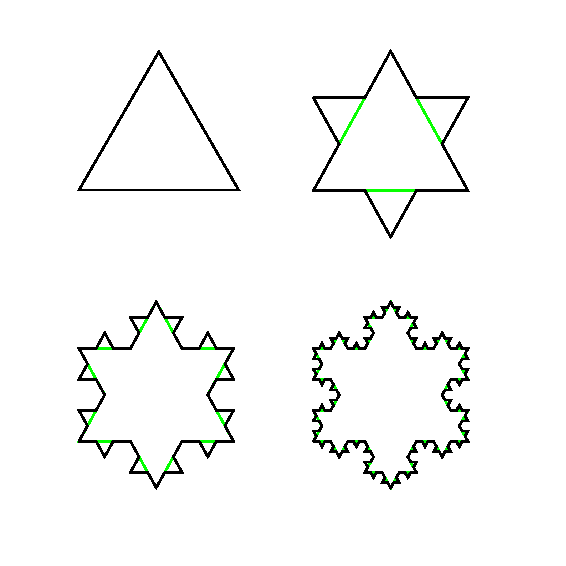
\includegraphics[width=0.5\linewidth]{Figures/Chapter2/fig_koch}
\caption{The procedure for constructing a Koch snowflake, a good example of exact self-similarity.  \href{https://commons.wikimedia.org/wiki/File:KochFlake.svg}{(Image: Wxs, CC BY-SA 3.0.)} }
\label{fig_koch}
\end{figure}

\begin{figure}
\centering
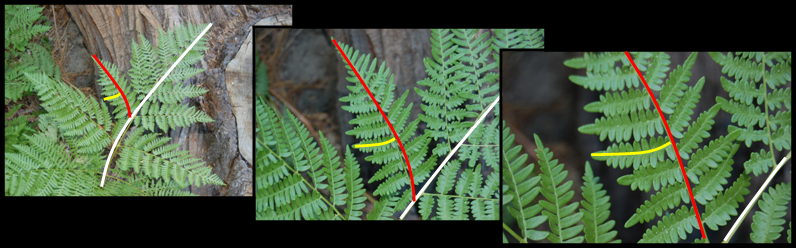
\includegraphics[width=1\linewidth]{Figures/Chapter2/fig_fern.png}
\caption{A fern is an example of self-similarity found in nature.  \href{https://www.flickr.com/photos/78523101@N04/7572281628}{(Photo: Jason Hine, CC BY-NC 2.0.)} }
\label{fig_fern}
\end{figure}

It's time to exploit this idea mathematically.  Let's define a new variable,
\begin{equation}
\eta = \frac{y}{\sqrt{\nu t}}.
\end{equation}
Our goal will be to rewrite the partial differential equation (\ref{eq_ss_diffeq_tilde}) in terms of $\eta$ rather than $y$ and $t$.  We can do this with the chain rule, so that
\[
\dfdx{\tilde{u}}{t} = \frac{df}{d\eta} \dfdx{\eta}{t} = -\frac{y}{2 \nu^{1/2} t^{3/2}} f',
\]
where the prime indicates a derivative with respect to $\eta$, and
\[
\ddfdx{\tilde{u}}{y} = \frac{d^2 f}{d\eta^2} \left( \dfdx{\eta}{y} \right)^2 + \dfdx{f}{\eta} \ddfdx{\eta}{y} = \left( \frac{1}{\nu t} \right) f''.
\]
Careful with the second derivative calculation -- it uses a product rule as well as the chain rule, so go over it yourself to make sure you know where the terms come from.  Plugging these two derivatives back into equation (\ref{eq_ss_diffeq_tilde}) gives, after a bit of rearranging,
\begin{equation}
f'' + \frac{1}{2} \eta f' = 0.
\end{equation}
As promised, we now have only one ordinary differential equation to worry about -- and note that this equation contains only dimensionless quantities.

It's straightforward to solve this differential equation as well.  First, let
\[
g = f',
\]
so that $g' = f''$, and the equation becomes the first order
\[
g' + \frac{1}{2} \eta g = 0.
\]
Writing all the $g$s on one side and the $\eta$s on the other allows us to integrate it, to get
\[
g(\eta) = f' = B e^{-\tfrac{1}{4} \eta^2},
\]
where $B$ is the integration constant.  Integrating one more time will get us $f(\eta$),
\[
f(\eta) = A + B \int_0^\eta e^{-\tfrac{1}{4} \eta'^2} \, d\eta'.
\]
Here, $A$ is another integration constant (to account for the definite integral), and I've written $\eta'$ as the integration variable to avoid confusion.  Unfortunately, actually solving the integral in this equation is not possible in closed form -- in fact, the integral
\[
\frac{1}{\sqrt{\pi}} \int_0^x e^{-\tfrac{1}{4} u^2} du \equiv \text{erf}(x),
\]
is called the \emph{error function}, and is used extensively in probability and statistics.  Since we can only evaluate the error function numerically, I'll continue to just write out the integral.

We can find the constants $A$ and $B$ with our boundary conditions and the initial condition.  Before we do that, though, we need to express them in terms of $\eta$ rather than $y$ and $t$.  The first boundary condition is
\[
\tilde{u}(0, t) = 1.
\]
But at this place ($y=0$) and time ($t$), we have $\eta = 0$,  so the boundary condition for $\eta=0$ becomes
\[
f(0) = 1.
\]
The second boundary condition likewise becomes
\[
f(\infty) = 0.
\]
Also, recall that the initial condition was $\tilde{u}(y, 0) = 0$.  In this case, $\eta \to \infty$, since $t$ is in the denominator, and we get again the same expression as the second boundary condition -- as expected, we have only two boundary conditions for our second order differential equation.

Using these two boundary conditions leads to $A=1$ and $B = -1/\sqrt{\pi}$.  We can write our final solution, then (using $u = U\tilde{u}$), as
\begin{equation}
u(y, t) = f(\eta) = U\left[ 1 - \frac{1}{\sqrt{\pi}} \int_0^\eta e^{-\tfrac{1}{4} \eta'^2} d\eta' \right],
\end{equation}
where, of course, $\eta = y / \sqrt{\nu t}$.

We can take a look at the velocity for a couple of different times to see how the fluid responds to the impulsively moved boundary -- see Figure \ref{fig_ss_vel1}.  As expected, at later time the fluid is moving faster, and \emph{more} of the fluid is moving.  This is evident in Figure \ref{fig_ss_vel1}; at $t=1$, the fluid above $y \sim 3$ practically isn't moving, while for $t=10$, the motion of the fluid extends up to $y \sim 10$.

\begin{figure}
\centering
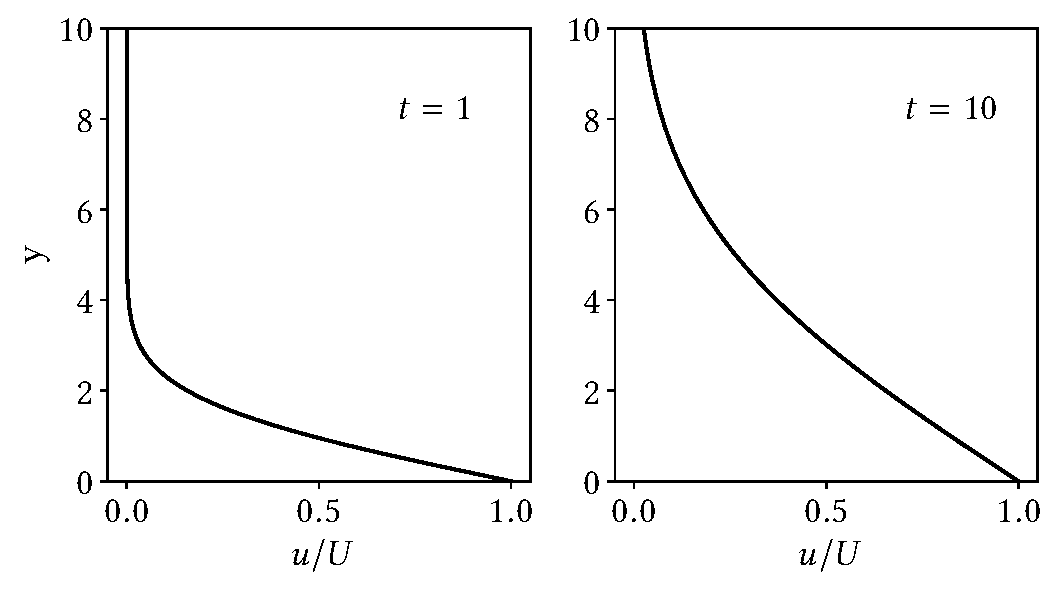
\includegraphics[width=0.8\linewidth]{Figures/Chapter2/fig_ss_vel1}
\caption{The fluid velocity for an impulsively moved boundary at $y=0$.  Note how long it takes for the fluid to respond -- at the later time on the right (ten times longer than the left), the velocity has increased at all points but still drops to zero around $y=10$.  I set $\nu = 1$ for convenience.}
\label{fig_ss_vel1}
\end{figure}

I mentioned earlier that this solution would be self-similar, but that's not very noticeable in Figure \ref{fig_ss_vel1}.  That's because both time \emph{and} space must be scaled together to get the same velocity curve.  In fact, if we zoom out on the $y$-axis as we move forward in time, the motion of the fluid should always be the same.  We can see that in Figure \ref{fig_ss_vel2}, which changes the scale of the $y$-axis for the right-hand plot at $t=10$.  Rather than going from $y=0$ to $y=10$, as in Figure \ref{fig_ss_vel1}, we go from $y=0$ to
\[
y = {10}{\sqrt{\nu t}}
\]
(remember, $\eta = y / \sqrt{\nu t}$).  Thus, as $t$ changes, so too does the scale of $y$.  In this case, both velocity curves look identical, and the solution is self-similar.

\begin{figure}
\centering
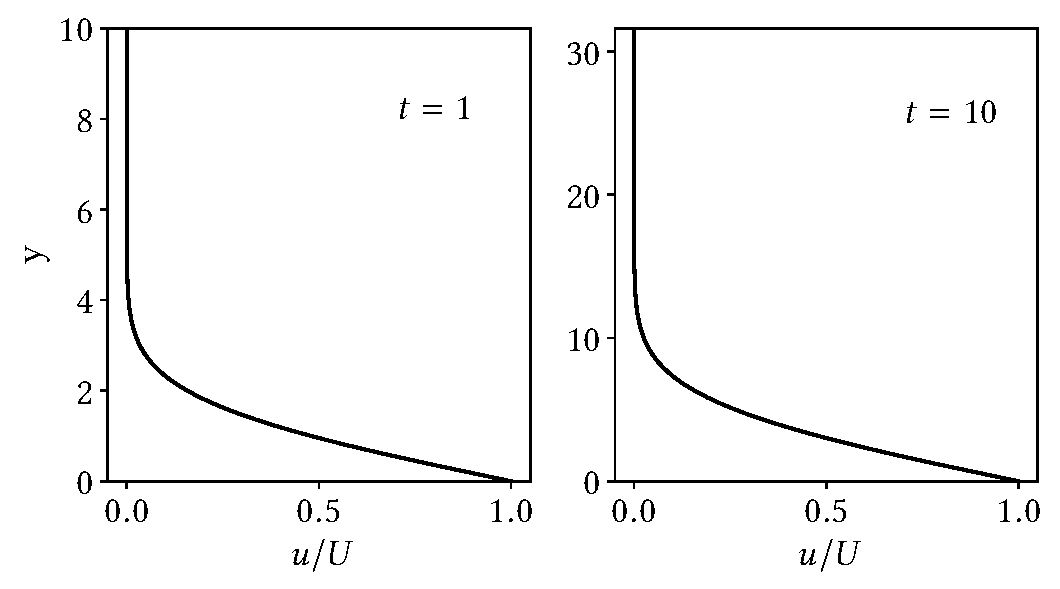
\includegraphics[width=0.8\linewidth]{Figures/Chapter2/fig_ss_vel2}
\caption{The fluid velocity for an impulsively moved boundary at $y=0$.  This time, I've changed the $y$-axis scale so that the two curves are self-similar. }
\label{fig_ss_vel2}
\end{figure}


%
% --- SECTION - CIRCULAR FLOW ---
% 

\section{Circular Flow}


% SUBSECTION - THE NS EQs IN CYLINDRICAL

\subsection{The Navier-Stokes Equations in Cylindrical Coordinates}
\label{sec_ns_cyl}

The Navier-Stokes equations are trickier to write down in cylindrical coordinates, mainly due to the fact that the cylindrical unit vectors $\unit{s}$ and $\unit{\phi}$ in equation (\ref{eq_u_cyl}) are not \emph{constant} -- they depend on $\phi$:
\begin{align*}
\unit{r} & = \cos \phi \unit{x} + \sin \phi \unit{y}, \\
\unit{\phi} & = - \sin \phi \unit{x} + \cos \phi \unit{y}.
\end{align*}
When evaluating the derivatives in the Navier-Stokes equation, then, you have to be very careful to take this dependence into account.  For example, note that
\[
\frac{d\unit{s}}{d\phi} = \unit{\phi}
\]
and
\[
\frac{d\unit{\phi}}{d\phi} = - \unit{s}.
\]

Furthermore, the gradient and Laplacian operators in cylindrical coordinates are a little more cumbersome than in Cartesian; I won't bother writing them out here, but you should look them up on your own.\footnote{I really like the front and back covers in Griffiths' \emph{Introduction to Electrodynamics} for this.}  Altogether, here's the Navier-Stokes equations in cylindrical coordinates for you:
\begin{align}
\label{eq_ns_r}
\frac {\partial u_{s}}{\partial t} + (\vec{u} \cdot \grad) u_{s} - \frac {u_{\phi}^{2}}{s} & = - \frac {1}{\rho} \frac {\partial p}{\partial s} + \nu \left (\nabla^{2} u_{s} - \frac {u_{s}}{s^{2}} - \frac {2}{s^{2}} \frac {\partial u_{\phi}}{\partial \phi} \right) +  g_s\\
\label{eq_ns_theta}
\frac {\partial u_{\phi}}{\partial t} + (\vec{u} \cdot \grad) u_{\phi} + \frac {u_{s} u_{\phi}}{s} & = - \frac {1}{\rho s} \frac {\partial p}{\partial \phi} + \nu \left (\nabla^{2} u_{\phi} - \frac {u_{\phi}}{s^{2}} + \frac {2}{s^{2}} \frac {\partial u_{s}}{\partial \phi} \right) + g_\phi\\
\label{eq_ns_z}
\frac {\partial u_{z}}{\partial t} + (\vec{u} \cdot \grad) u_{z} & = -\frac {1}{\rho} \frac {\partial p}{\partial z} + \nu \nabla^{2} u_{z} + g_z \\
\end{align}
where
\begin{align}
(\vec{u} \cdot \grad) & = u_{s} \frac {\partial}{\partial s} + \frac {u_{\phi}}{s} \frac {\partial}{\partial \phi} + u_{z} \frac {\partial}{\partial z}, \\
\nabla^{2} & = \frac {1}{s} \frac {\partial}{\partial s} \left (s \frac {\partial}{\partial s} \right) + \frac {1}{s^{2}} \frac {\partial^{2}}{\partial \phi^{2}} + \frac {\partial^{2}}{\partial z^{2}}.
\end{align}
In addition, the incompressibility condition $\grad \cdot \vec{u} = 0$ becomes 
\begin{equation}
\frac {1}{s} \frac {\partial}{\partial s} (s u_{s}) + \frac {1}{s} \frac {\partial u_{\phi}}{\partial \phi} + \frac {\partial u_{z}}{\partial z} = 0.
\end{equation}


% SUBSECTION - UNIFORMLY ROTATING FLUID

\subsection{Uniformly Rotating Fluid}
\label{sec_uni_rot_fluid}

For our first problem, we'll consider fluid within a cylinder of radius $a$, as shown in Figure \ref{fig_cyl_setup}, with the cylinder rotating with an angular speed $\Omega$. 

Already this is two dimensional flow -- we'll assume the cylinder is infinitely long, so there won't be any $z$ dependence of the flow in that direction.  To make things simpler, we'll also impose full cylindrical symmetry on our flow:  the velocity will always take the form
\begin{equation}
\vec{u} = u_\phi (s, t) \, \unit{\phi}.
\end{equation}
This means that the flow is always \emph{circular}, with streamlines that are circles.  Furthermore, the speed of the fluid only depends on the distance $s$ from the origin, giving us the cylindrical symmetry.  One nice benefit to a flow of this form is that the incompressibility condition is automatically satisfied, which you can check yourself with Problem \ref{prob_cyl_incomp}.

\begin{figure}
\centering
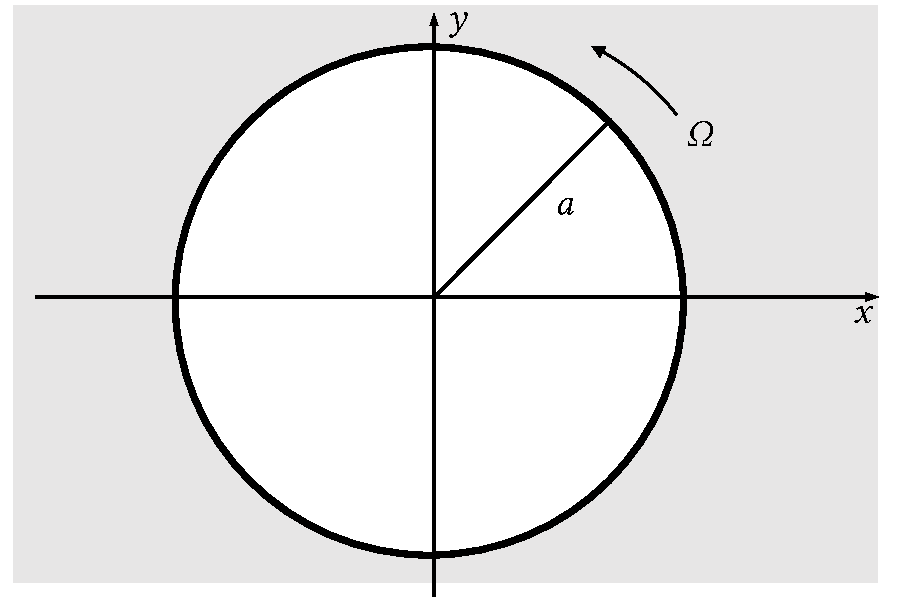
\includegraphics[width=0.7\linewidth]{Figures/Chapter2/fig_cyl_setup}
\caption{The fluid is constrained to be within a cylinder of radius $a$.  We'll put the origin at the centre of the cylinder.}
\label{fig_cyl_setup}
\end{figure}

As you might expect, taking this form of the velocity drastically reduces the Navier-Stokes equations.  Equations \ref{eq_ns_r} - \ref{eq_ns_z} become
\begin{align}
\frac{u_\phi^2}{s} & = \frac{1}{\rho} \dfdx{p}{s} \\
\label{eq_ns_theta2}
\dfdx{u_\phi}{t} & = -\frac{1}{\rho s} \dfdx{p}{\phi} + \nu \left( \ddfdx{u_\phi}{s} + \frac{1}{s} \dfdx{u_\phi}{s} - \frac{u_\phi}{s^2} \right) \\
\label{eq_ns_z2}
0 & = -\frac{1}{\rho} \dfdx{p}{z}.
\end{align}
Note that I've completely dropped the gravity terms here -- but see Problem \ref{prob_poise_grav} for the minimal effect that gravity has on our problems.

Now, the third equation above -- the one for $z$ -- just says that the pressure $p$ doesn't depend on $z$ at all, not surprising given the symmetry of the problem.  The first equation gives us a relationship between the fluid velocity $u_\phi$ and the radial pressure gradient, so if we know one we can get the other.  The second equation is the important one, but we can clean it up a bit more.  

Since $u_\phi = u_\phi(s, t)$ only, equation (\ref{eq_ns_theta2}) says that $\partial p / \partial \phi$ must also be a function of only $s$ and $t$.  So we can write
\[
\dfdx{p}{\phi} = P(s, t),
\]
where $P(s, t)$ is some unknown function.  If we integrate this to find $p$, we get
\[
p = P(s, t) \phi + f(s, t),
\]
where $f(s, t)$ is the integration ``constant'' -- remember, we have a partial derivative here (and note that there's no $z$ dependence thanks to equation (\ref{eq_ns_z2})).  But this shows us that the function $P(s, t)$ \emph{must} be zero, since otherwise the pressure would be a multivalued function of position; it would take on different values for $\phi = 0$ and $\phi = 2 \pi$, for example, even though those two angles represent the same point in space.

Equation (\ref{eq_ns_theta2}) then becomes, with $P(s, t) = \partial p / \partial \phi = 0$, 
\begin{equation}
\label{eq_ns_evol}
\boxed{
\dfdx{u_\phi}{t} =  \nu \left( \ddfdx{u_\phi}{s} + \frac{1}{s} \dfdx{u_\phi}{s} - \frac{u_\phi}{s^2} \right).
}
\end{equation}
This equation determines the evolution of the fluid velocity, and holds for any flow with circular streamlines.

Now we can go back to our original problem -- fluid inside a rotating cylinder.  We'll first assume the fluid is \emph{steady}, so that $\partial u_\phi / \partial t = 0$.  Multiplying equation (\ref{eq_ns_evol}) by $s^2$ gives us
\begin{equation}
\label{eq_spin_diffeq}
s^2 \frac{d^2 u_\phi}{ds^2} + s \frac{d u_\phi}{ds} - u_\phi = 0.
\end{equation}
Notice that the viscosity has dropped out of the problem.  To solve this ordinary differential equation, let's ``guess'' at a power-law solution of the form
\[
u_\phi(s) = s^m.
\]
Plugging this form into our equation leads to the quadratic 
\[
m^2 -1 = 0,
\]
which has roots $m = +1$ and $m = -1$.  Our general solution is then
\begin{equation}
\label{eq_cyl_steady_gen_sol}
u_\phi (s) = As + \frac{B}{s}.
\end{equation}

Since we have viscous fluid, one of our boundary conditions must be that the fluid moves with the same velocity as the cylinder wall, so that
\[
u_\phi(a) = \Omega a.
\]
We don't really have another boundary condition, since there isn't another boundary; however, note that the second term in Equation \ref{eq_cyl_steady_gen_sol} blows up at $s=0$, the centre of the cylinder.  So, to keep the fluid velocity everywhere finite, we need to set $B = 0$.  The boundary condition then leads to $A = \Omega$, so our solution is 
\begin{equation}
\label{eq_cyl_steady_sol}
u_\phi (s) = \Omega s.
\end{equation}
This flow is in \emph{solid body rotation} -- in other words, the fluid rotates in exactly the same way as a solid body would, at constant angular speed $\Omega$.


% SUBSECTION - SPIN DOWN

\subsection{Spin Down of Rotating Fluid}

What happens to the fluid if the rotating cylinder is suddenly brought to rest?  Now we have time-dependent flow, and we'll have to use the full equation (\ref{eq_ns_evol}) to model what happens.  Just a warning before we proceed:  this is a pretty complicated problem to solve, and will require some knowledge about Bessel functions.  We'll take it slow, but it might help to read up on them first.

We'll use separation of variables to solve the partial differential equation, but first we should write out the initial and boundary conditions.  The initial condition is of course our steady state solution we just found, equation (\ref{eq_cyl_steady_sol}),
\begin{equation}
\label{eq_spin_ic}
u_\phi (s, t=0) = \Omega s.
\end{equation}
We'll suppose the cylinder is brought to rest at $t=0$, so after that the no-slip condition says that
\begin{equation}
u_\phi(a, t) = 0 \quad \text{for } t > 0.
\end{equation}
As with our last problem, we'll also have to make sure that the velocity is finite everywhere in the fluid.

Let
\[
u_\phi(s, t) = S(s) T(t)
\]
and plug that into equation (\ref{eq_ns_evol}).  Dividing both sides by $ST$ gives
\[
\frac{1}{\nu T} \frac{dT}{dt} = \frac{1}{S} \frac{d^2S}{ds^2} + \frac{1}{sS} \frac{dS}{ds} - \frac{1}{s^2}.
\]
The left hand side is a function of time $t$ only, while the right hand side depends only on $s$.  Since they're independent variables, both sides must be equal to a constant, which, with the benefit of hindsight, we'll call $-k^2$.

The left hand side becomes
\[
 \frac{dT}{dt} = -\nu k^2 T,
\]
which has the solution
\begin{equation}
T(t) = C e^{-\nu k^2 t},
\end{equation}
where $C$ is a constant.  The right hand side is a little more difficult.  With a little manipulation (multiplying both sides by $s^2 S$) we can write it as
\[
s^2 \frac{d^2S}{ds^2} + s\frac{dS}{ds} + \left( k^2 s^2 - 1 \right) S = 0.
\]
One more small change:  let 
\[
x = k s.
\]
Then the equation becomes
\begin{equation}
\label{eq_bessel}
x^2 \frac{d^2S}{dx^2} + x\frac{dS}{dx} + \left(  x^2 - 1 \right) S = 0.
\end{equation}
This equation isn't easy to solve by hand, but it turns out to be a fairly famous differential equation that pops up in various places in physics (like electromagnetism and acoustics) -- it's called Bessel's equation, and the solutions are called \emph{Bessel functions}.

The Bessel function of the first kind is usually written $J_\alpha(x)$, where $\alpha$ is called the \emph{order} of the Bessel function.  In our case, with the $(x^2 - 1)$ term in the equation, we're dealing only with the first order, so $\alpha = 1$.  The second solution is the Bessel function of the second kind, sometimes called the Neumann function, $Y_\alpha(x)$.  We can't write either function in closed form -- the best we can do is a series solution -- but I've plotted both $J_1(x)$ and $Y_1(x)$  in Figure \ref{fig_bessel}.  Note that both functions are oscillatory, but not with a nice regular period like sine and cosine; Table \ref{tab_bessel} lists a few of the zeros of each, and we'll need those in a moment.

\begin{figure}
\centering
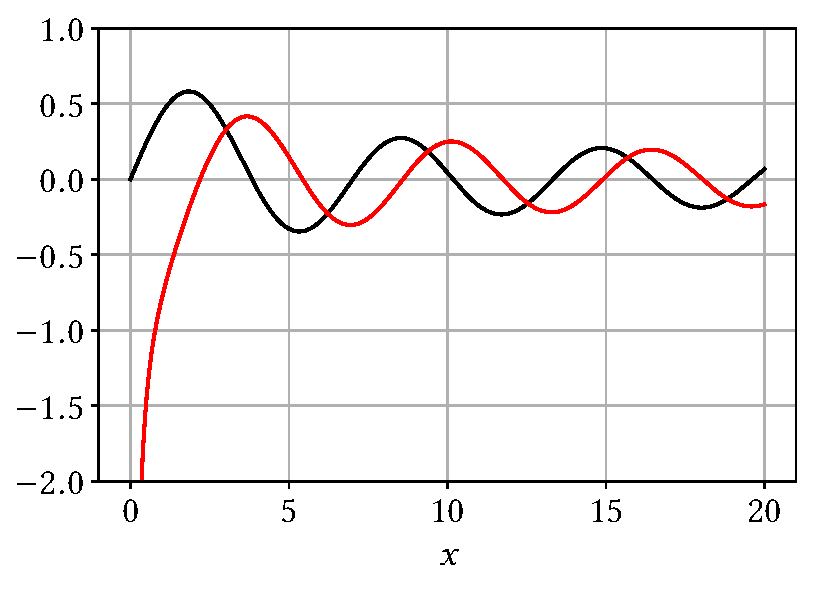
\includegraphics[width=0.7\linewidth]{Figures/Chapter2/fig_bessel}
\caption{The Bessel functions of the first ($J_1(x)$, black) and second ($Y_1(x)$, red) kind, of order $\alpha = 1$.}
\label{fig_bessel}
\end{figure}

\begin{table}[t]
\centering
  \begin{tabular}{l|l|l}
  & $J_1(x)$ & $Y_1(x)$ \\
  \hline \\
   $\lambda_1$ & 3.83170597   & 2.19714133    \\
   $\lambda_2$ & 7.01558667 & 5.42968104   \\
   $\lambda_3$ & 10.17346814 & 8.59600587  \\
   $\lambda_4$ & 13.32369194 & 11.74915483 \\
   $\lambda_5$ & 16.47063005 & 14.89744213
  \end{tabular}
  \caption{The first five zeros for the Bessel functions.}
  \label{tab_bessel}
\end{table}

The general solution to Equation \ref{eq_bessel} is the superposition of both Bessel functions, 
\[
S(x) = A J_1(x) + B Y_1(x).
\]
However, we can see from Figure \ref{fig_bessel} that $Y_1(x)$ goes to negative infinity at the origin.  This is no good -- we want the velocity of the fluid to always be finite -- so we can drop the this function and set $B=0$.  Going back to using $s$ instead of $x$, we have
\[
S(s) = A J_1(ks).
\]

Now we can apply our boundary condition at $s=a$.  I'll write it out for you:
\[
S(a) = A J_1 (ka) = 0.
\]
Clearly, we can't set $A=0$, since that will give us a static fluid; instead, we'll have to use the fact that the Bessel function has an infinite number of zeros, just like we did with the sine function back in Section \ref{sec_imp}.  Unfortunately, the Bessel zeros aren't at nicely periodic locations like $n\pi$; as you can see in Table \ref{tab_bessel}, they're neither periodic nor at nice locations.  Instead, we'll have to be more general, so I'll call the $n$th zero of the Bessel function $\lambda_n$.  That is, 
\[
J_1(\lambda_n) = 0
\]
for every value of $\lambda_n$.  The boundary condition thus implies that $ka = \lambda_n$, or
\[
k = \frac{\lambda_n }{a}.
\]

Let's put our solution so far together.  We'll combine the results for $T(t)$ and $S(s)$ to get the fluid velocity
\[
u_\phi(s, t) = S(s) T(t) = A \, J_1(\lambda_n s / a) \, e^{-\lambda_n^2 \nu t /a^2},
\]
where I've combined the two constants into $A$.  As is usual with separation of variables, we end up with not just \emph{one} solution, but an \emph{infinite} number of them.  That means the most general solution is a linear combination of all of them,
\begin{equation}
u_\phi(s, t) = \sum_{n=1}^\infty A_n \, J_1(\lambda_n s / a) \, e^{-\lambda_n^2 \nu t /a^2}.
\end{equation}

Even though we've been dealing with Bessel function, the process of separation of variables is the same as we went through in Section \ref{sec_poise_time} -- if you can follow that discussion, you should be okay here, too.  We just have one more step:  finding the values of the constants $A_n$ that will match our initial conditions.  This part is similar to before, too, but does require a bit of advanced knowledge of Bessel functions, so watch carefully.

Our initial conditions, from equation (\ref{eq_spin_ic}), say
\begin{equation}
\label{eq_spin_ic2}
u_\phi(s,0) =  \sum_{n=1}^\infty A_n \, J_1(\lambda_n s / a) = \Omega s.
\end{equation}
Just like sinusoidal functions, Bessel functions are orthogonal, although it looks a little different; it turns out that\footnote{See, for example, Arfken and Weber's \emph{Mathematical Methods for Physicists}, Fourth Edition, p. 646.}
\[
\int_0^a J_1(\lambda_n s / a) J_1(\lambda_m s /a) \, s\, ds = 0
\]
if $m \neq n$.  If $m = n$, then the result is
\[
\int_0^a J_1^2(\lambda_n s / a) \, s \, ds = \frac{a^2}{2} J_2^2(\lambda_n)
\]
(notice that's the second order Bessel function showing up on the right hand side).

We can use these results to solve for the $A_n$s.  Multiply both sides of equation (\ref{eq_spin_ic2}) by $s J_1(\lambda_m s /a)$ and integrate from $0$ to $a$:
\[
\sum_{n=1}^\infty A_n \int_0^a J_1(\lambda_n s / a) J_1(\lambda_m s /a) \, s\, ds = \Omega \int_0^a s^2 \, J_1(\lambda_m s/a) \, ds.
\]
Orthogonality allows us to collapse the sum -- only the $m$th term survives -- and, performing the integrations, we get
\[
A_n = \frac{2 \Omega a}{\lambda_n \, J_2(\lambda_n)}.
\]

Putting this result together with our general solution gives us, finally,
\begin{equation}
u_\phi(s, t) = 2\Omega a \sum_{n=1}^\infty \frac{J_1(\lambda_n s/a)}{\lambda_n J_2(\lambda_n)} \, e^{-\lambda_n^2 \nu t / a^2}.
\end{equation}
Unlike our steady state solution, this one depends on the viscosity of the fluid -- it controls how long it takes for the fluid to slow down.  I've plotted the velocity in Figure \ref{fig_spin_vel}, where you can see how the fluid behaves over time, but it might be useful to take a more physical look at this problem.  I have a water bottle on my desk right now, half-filled with water, with a radius of about $4$ cm.  The viscosity of water, from Table \ref{tab_viscosity}, is $\nu = 0.01$ cm$^2$/s.  Taking, as we did before, the first term only in the sum, 
\[
u_\phi(s, t) \approx \frac{2\Omega a J_1(\lambda_1 s/a)}{\lambda_1 J_2(\lambda_1)} \, e^{-\lambda_1^2 \nu t / a^2}.
\]
It's the exponential term we really want to look at; the characteristic time is
\[
\tau = \frac{a^2}{\nu \lambda_1^2} \approx 110 \text{ s}.
\]
That's a long time for my water bottle to slow down once I've rotated up to some speed.  However, when I eyeball it, it looks like it takes about 25 s to come to a complete stop -- much quicker!  The thing we're missing in our analysis, of course, is the \emph{bottom} of the bottle -- it apparently plays an important role in the spin down of the water in the bottle.

\begin{figure}
\centering
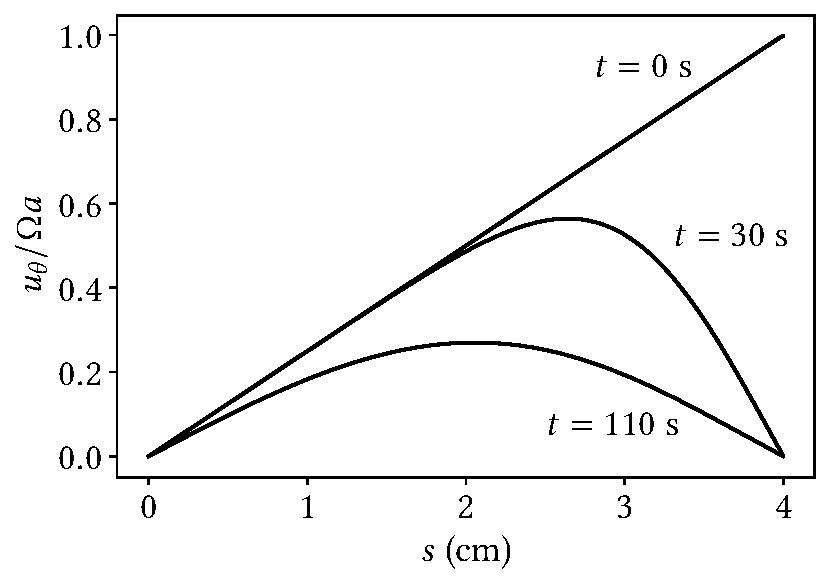
\includegraphics[width=0.7\linewidth]{Figures/Chapter2/fig_spin_vel}
\caption{The spin down of fluid initially rotating like a solid body at three different times. In this case, I set $a = 4$ cm and $\nu = 0.01$ cm$^2$/s as in the water bottle example.}
\label{fig_spin_vel}
\end{figure}


% SUBSECTION - THE LINE VORTEX

\subsection{The Line Vortex}
\label{sec_line_vortex}

Our last two examples involved fluid \emph{inside} a cylinder; let's flip that around and look at the fluid \emph{outside} a solid cylinder, rotating initially at some angular speed $\Omega$ (see Figure \ref{fig_line_setup}).  As we've done a number of times in this chapter, we'll search first for a steady-state solution, and then look at time-dependence.

\begin{figure}
\centering
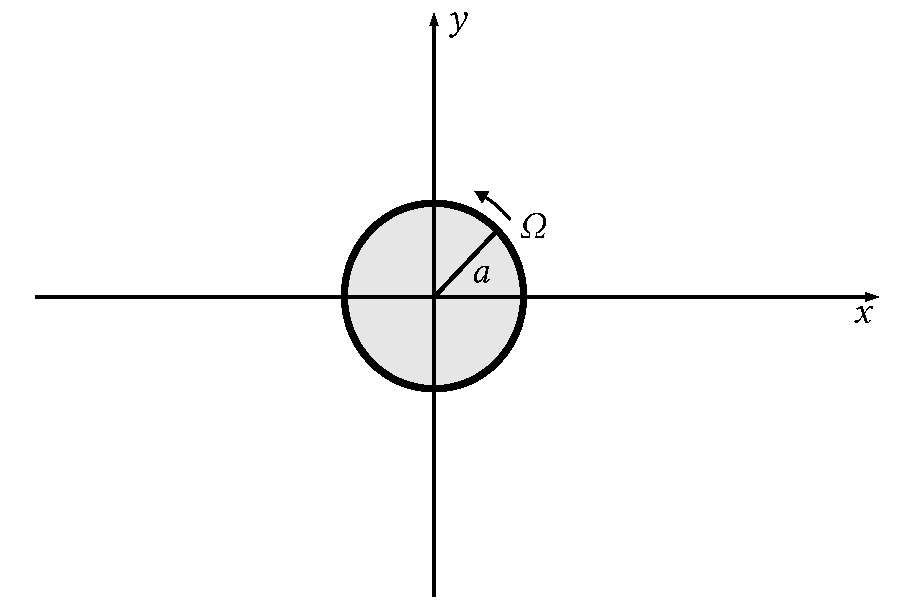
\includegraphics[width=0.7\linewidth]{Figures/Chapter2/fig_line_setup}
\caption{A solid cylinder rotating in a fluid.}
\label{fig_line_setup}
\end{figure}

We once again have circular flow, and the steady-state is described by equation (\ref{eq_spin_diffeq}) and its general solution, equation (\ref{eq_cyl_steady_gen_sol}),
\[
u_\phi (s) = As + \frac{B}{s}.
\]
Although the boundary condition is \emph{also} the same -- that $u_\phi(a) = \Omega a$ -- the difference here comes from keeping the fluid velocity finite.  Since the fluid extends out to infinity, we set $A = 0$; with no fluid at $s=0$, the second term won't be a problem.  Fitting the boundary condition leads to our answer,
\[
u_\phi(s) = \frac{\Omega a^2}{s}.
\]

We've seen this kind of flow before -- it's the line vortex from Example \ref{ex_vorticity_line_vortex}, with $k=\Omega a^2$.  In fact, it's customary to write this flow as
\begin{equation}
\label{eq_line_vortex}
u_\phi(s) = \frac{\Gamma_0}{2\pi s},
\end{equation}
where the constant $\Gamma_0$ is called the \emph{circulation}.  We'll explore the concept of circulation more later on in the book.

Now let's take the cylinder away.  But we'll do it carefully -- we'll let $a \to 0$ at $t=0$, and the radius will shrink to zero instantaneously (kind of like how the boundary started moving in Section \ref{sec_imp}).  That means equation (\ref{eq_line_vortex}) will give us the initial conditions, but now the evolution of the system is governed by equation (\ref{eq_ns_evol}),
\[
\dfdx{u_\phi}{t} =  \nu \left( \ddfdx{u_\phi}{s} + \frac{1}{s} \dfdx{u_\phi}{s} - \frac{u_\phi}{s^2} \right).
\]

Before we solve this, I want to make a small change to this differential equation.  Let's define a new variable,
\begin{equation}
\Gamma (s, t) = 2\pi r u_\phi(s, t).
\end{equation}
Then, with a bit of work, the evolution equation becomes slightly simpler,
\begin{equation}
\label{eq_evol_gamma}
\dfdx{\Gamma}{t} = \nu \left( \ddfdx{\Gamma}{s} - \frac{1}{s} \dfdx{\Gamma}{s} \right),
\end{equation}
and the initial conditions are now given by
\begin{equation}
\Gamma(r, 0) = \Gamma_0.
\end{equation}

What about the boundary conditions?  Well, as usual we want the flow to be finite everywhere for $t>0$ (careful -- right \emph{at} $t=0$ the flow $u_\phi$ is in fact infinite, a point we'll discuss in the next section).  With our definition of $\Gamma$, that means we need
\begin{equation}
\Gamma(0, t) = 0 \quad \text{for } t>0.
\end{equation}

Now we're ready to solve this problem.  Note that it's actually \emph{scale-free} -- there's nothing here (once the cylinder disappears) to provide any physical scale.  That suggests we can seek a self-similar solution. As we did before in Section \ref{sec_self_similar}, we can define a new dimensionless variable,
\begin{equation}
\eta = \frac{s}{\sqrt{\nu t}},
\end{equation}
and assume that the solution is some function a $\eta$ alone,
\[
\Gamma(s, t) = f(\eta).
\]
I'll let you plug this into equation (\ref{eq_evol_gamma}) and find the similarity solution yourself (Problem \ref{prob_sim}).  The answer is
\[
\Gamma(s, t) = \Gamma_0 \left(1 - e^{-s^2 / 4\nu t} \right),
\]
so that the fluid velocity is
\begin{equation}
\label{eq_line_vortex_vel}
u_\phi(s, t) = \frac{\Gamma_0}{2\pi s} \left( 1- e^{-s^2 / 4 \nu t} \right).
\end{equation}

Let's explore this solution a bit.  I've plotted the velocity in Figure \ref{fig_line_vortex} for a couple of different times so you can see how the speed decays.  For large radii, $s \gg \sqrt{4\nu t}$, we can drop the exponential term in Equation \ref{eq_line_vortex_vel}, and the behaviour far from the origin still looks like a line vortex:
\[
u_\phi \approx \frac{\Gamma_0}{2\pi s}.
\]
However, at small radii, $s \ll \sqrt{4 \nu t}$, we can expand the exponential and, keeping only the first two terms, get
\[
u_\phi \approx \left( \frac{\Gamma_0}{8 \pi \nu t} \right) s.
\]
This looks like solid body rotation again, with $u_\phi \propto s$.  Thus, at small radii, the flow is completely different; it undergoes solid body rotation and has \emph{vorticity}.  It's the role of vorticity we need to discuss next.

\begin{figure}
\centering
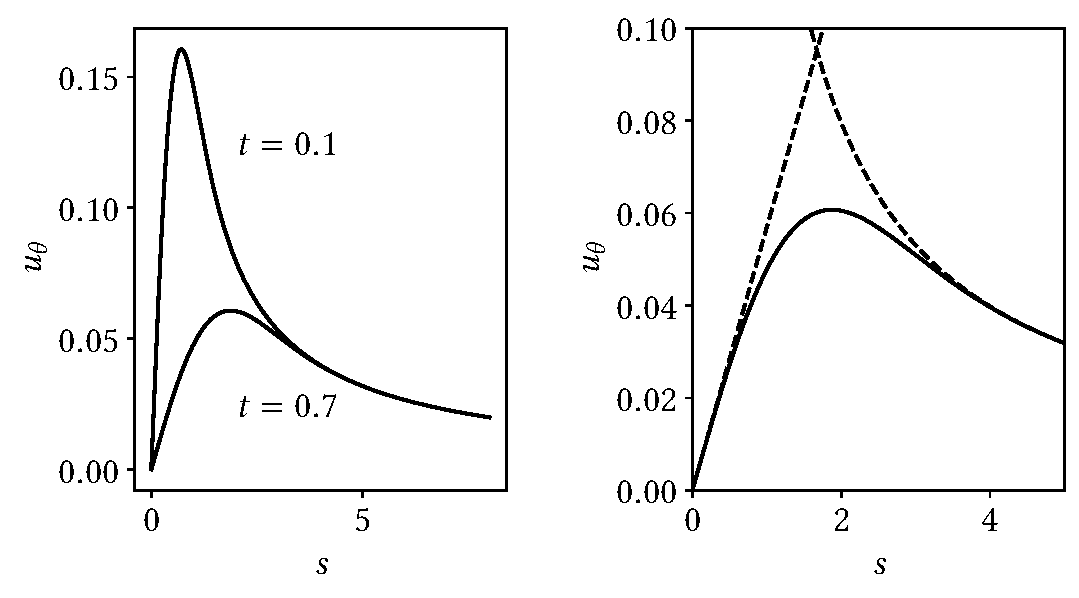
\includegraphics[width=0.8\linewidth]{Figures/Chapter2/fig_line_vortex}
\caption{The decay of a line vortex.  On the left plot, the fluid velocity is shown at two different times.  On the right plot, just $t=0.7$ is shown, along with the small- and large- radii behaviour shown as dashed lines. For convenience, I set $\Gamma_0 = 1$ and $\nu = 1$.}
\label{fig_line_vortex}
\end{figure}

%
% --- SECTION - Transport of Vorticity ---
% 

\section{Transport of Vorticity}

So far, all we've done is solve the Navier-Stokes equations for a variety of different situations.  Actually, the variety hasn't been all that great -- we've really only covered two kinds of flow, \emph{plane parallel shear flow} and \emph{circular flow}.  In both cases, the flow direction is parallel to the flow dependence; in the case of plane parallel shear flow, we had the fluid moving in the $x$ direction, but the speed changed along the $y$ direction only.  For circular flow, the fluid flowed in the $\phi$ direction but all dependence was along the radius $s$.  

For flows of this type, the second term in the acceleration (equation (\ref{eq_accel})) -- the so-called convective term -- is zero:
\[
(\vec{u} \cdot \vec{\nabla}) \vec{u} = 0.
\]
This not only makes the Navier-Stokes equations significantly easier (it eliminates their nonlinear nature, for example), it also allows for only one kind of \emph{vorticity transport} as we'll see in a moment.

First, though, let's go back and take a look at two of our results:  the impulsively moved boundary in Section \ref{sec_self_similar} and the line vortex decay in Section \ref{sec_line_vortex}.  Both of these examples illustrated an interesting aspect concerning vorticity.  For the impulsively moved boundary, the vorticity is (see Problem \ref{prob_vorticity})
\begin{equation}
\label{eq_vort_1}
\omega = \frac{U}{\sqrt{\pi \nu t}} \, e^{-y^2 / 4 \nu t}.
\end{equation}
As $t \to 0$, the vorticity becomes infinite at the boundary $y=0$ but is zero everywhere else -- this is called a \emph{vortex sheet}.  The line vortex is similar, with 
\begin{equation}
\label{eq_vort_2}
\omega = \frac{\Gamma_0}{4\pi \nu t} \, e^{-s^2 / 4 \nu t}.
\end{equation}
This time, as $t \to 0$, the vorticity becomes infinite along $s=0$, but zero elsewhere, so this is a \emph{vortex line}.  Figure \ref{fig_vorticity_transport} shows the two vorticities at various times.  As you can see, the vorticity is strongly concentrated at either $y=0$ or $s=0$ at early times, but then becomes more ``spread out'' as time progresses.  It's this process of \emph{vorticity diffusion} that I want to discuss.

\begin{figure}
\centering
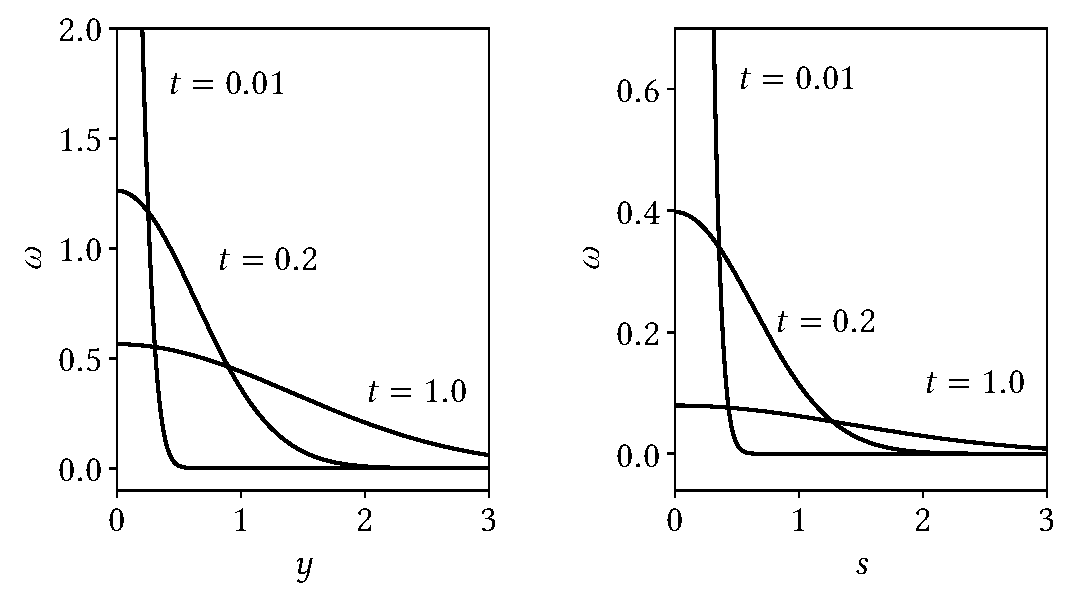
\includegraphics[width=0.8\linewidth]{Figures/Chapter2/fig_vorticity_transport}
\caption{The vorticity $\omega$ at a few different times for the impulsively moved boundary (left) and the line vortex (right).  In both cases an infinite amount of vorticity concentrated at one point spreads throughout the fluid.}
\label{fig_vorticity_transport}
\end{figure}

In fact, there are two different ways that vorticity can change in a fluid.  We can see this by taking the curl of both sides of the Navier-Stokes equations to get
\begin{equation}
\dfdx{\vort}{t} + (\vec{u} \cdot \grad) \vort = (\vort \cdot \grad) \vec{u} + \nu \nabla^2 \vort
\end{equation}
(this isn't exactly straightforward to derive, but we'll deal with it later in Section \ref{sec_vorticity_eq} for ideal fluids, and for now I don't want any distractions).  In two dimensional flow, like we've been dealing with in this chapter, it becomes a little simpler, since the first term on the right hand side will become zero -- the vector $\vort$ will point in the $z$ direction, so the term $\vort \cdot \grad$ will have only a $z$ derivative acting on $\vec{u}$, which of course only depends on $x$ and $y$.  That means this vorticity equation looks like
\[
\dfdx{\omega}{t} + (\vec{u}  \cdot \grad) \omega = \nu \left( \ddfdx{\omega}{x} + \ddfdx{\omega}{y} \right).
\]
We can now highlight the two ways that the vorticity can change:  first by viscous \emph{diffusion}, handled by the term with the viscosity in it, and second by \emph{convection}, which is the second term on the left.  By convection, I simply mean that the vorticity is transported through the fluid by the individual fluid elements themselves; in cases where the viscosity is zero, this is the only way to transport vorticity, and in that case each fluid element conserves its vorticity.

In all of the examples we've done so far, this convection term is zero, just like the convective acceleration is zero.  That means the vorticity is only transported through the fluid by diffusion.  In general, both mechanisms are at work, but of course those situations are significantly more difficult to deal with.  One example that's actually solvable -- with some difficulty and some numerical work -- is detailed in Section \ref{sec_boundary_layers}.



\section*{Problems}
\addcontentsline{toc}{section}{Problems}
\markright{Problems}%


\begin{problem}[Poiseuille flow with gravity]
\label{prob_poise_grav}
In Section \ref{sec_poise_1d} we examined Poiseuille flow in one dimension, but without the force of gravity playing a role.  Repeat our work to find the fluid velocity and pressure in the fluid, but this time include gravity in (a) the $x$ direction (so $\vec{g} = [g,0,0]$) and (b) the $z$ direction (so $\vec{g} = [0, 0, g]$).  Comment on how the velocity changes.  (\emph{Note:} you can still call the pressure gradient along the $x$ direction $P = -\partial p / \partial x$, but there could now also be addition dependence in the $z$ direction.)
\end{problem}

\begin{problem}[Flow down an incline]
Suppose fluid has been flowing down an inclined plane for a long time, as shown in Figure \ref{fig_incline_setup}.  The fluid has a height $h$ above the plane, and above the fluid is air.  Gravity points straight down, making an angle $\alpha$ with the $y$ axis.  What is the pressure and velocity of the fluid?  

\emph{Hint:} One of the boundary conditions is obvious, but the second is trickier.  Assume the pressure at the surface of the fluid is at atmospheric pressure, and also that there is no tangential stress across the surface (otherwise it wouldn't be a stable surface); see equation (\ref{eq_visc_def}).
\end{problem}

\begin{figure}
\centering
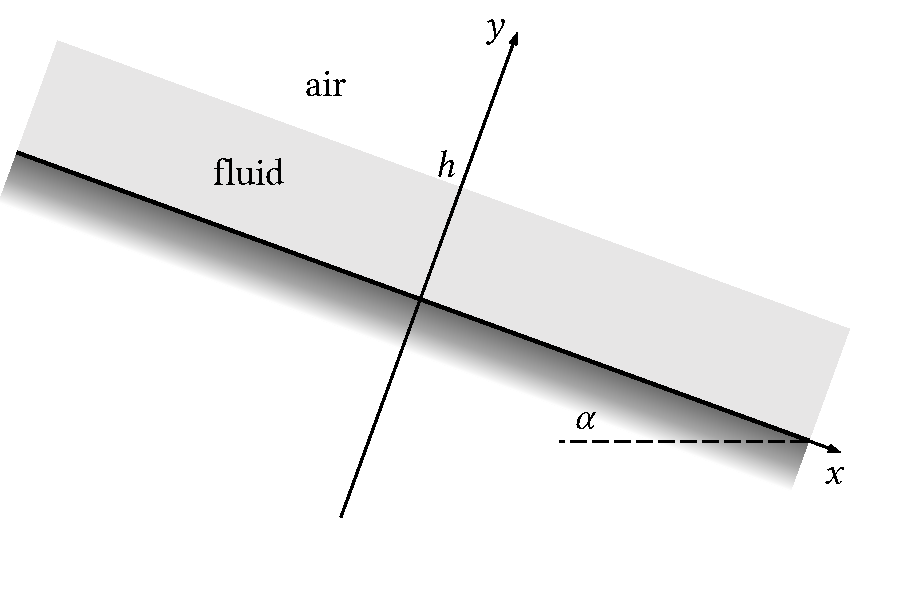
\includegraphics[width=0.7\linewidth]{Figures/Chapter2/fig_incline_setup}
\caption{Fluid flows down an incline.}
\label{fig_incline_setup}
\end{figure}

\begin{problem}[Poiseuille flow in two dimensions]
\label{prob_poise_2d}
Consider the rectangular pipe shown in Figure \ref{fig_poise_2d_setup}.  Suppose fluid flows down the $x$-axis thanks to a constant pressure gradient 
\[
\frac{dp}{dx} = -P,
\]
just as in the Poiseuille problem we discussed in Section \ref{sec_poise_1d}.  Find the velocity of the fluid within the pipe, and think about how to best visualize the flow.  

\emph{Hint:} The flow will now depend on $z$ as well as $y$, and the differential equation will be nonhomogeneous, so you'll have to figure out a way to \emph{make} it homogeneous.  Think about the 1D solution we did earlier.  This is a lengthy, difficult problem, so here's the final answer:
\begin{multline}
u(y, z) =  \frac{P}{2\nu \rho} \Biggl[ (ay - y^2) \, +  \\  \frac{8a^2}{\pi^3} \sum_{n=1,3,5, \dots} \frac{1}{n^3} \frac{1}{\cosh (n\pi b / 2a)} \sin (n\pi y / a) \cosh(n \pi z / a) \Biggr].
\end{multline}
\end{problem}

\begin{figure}
\centering
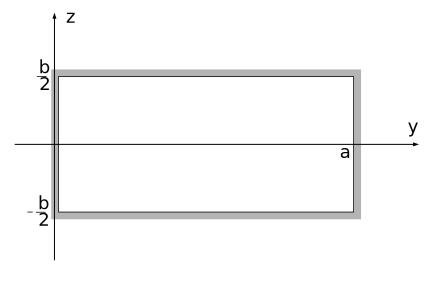
\includegraphics[width=0.7\linewidth]{Figures/Chapter2/fig_poise_2d_setup}
\caption{Fluid flows through a rectangular pipe.}
\label{fig_poise_2d_setup}
\end{figure}


\begin{problem}[Poiseuille flow in a cylinder]
\label{prob_poise_cyl}
The physician Poiseuille originally studied the problem of blood flowing through blood vessels. We can model that with a Newtonian fluid flowing down a pipe of circular cross-section (radius $a$).  If the pumping of the heart provides a constant pressure gradient within the blood vessel of $dp/dz = -P$,  find the velocity of the fluid.  Plot the velocity as a function of radius.
\end{problem}

\begin{problem}[Starting up Poiseuille flow]
\label{prob_poise_time}
For one last Poiseuille flow problem, consider the 1D example of Section \ref{sec_poise_1d} again.  This time, however, suppose that the fluid in the channel is at rest initially.  At time $t = 0$, the pressure gradient $dp/dx = -P$ starts instantaneously.  How does the fluid respond?  Find the velocity as a function of time, and plot it for a few different times.  What does the flow look like for $t \gg h^2 / \nu$?
\end{problem}

\begin{problem}[Fluid above an oscillating floor]
\label{prob_cyl_osc}
Fluid lies above an infinitely rigid plane at $y=0$.  The plane is oscillating back and forth along the $x$-direction with velocity
\[
u_\text{plane} = U \cos \omega t.
\]
Find the velocity of the fluid,\footnote{This is Stokes' second problem.} and plot it at some time $t$.  How far above the plane does the oscillatory motion seem to affect the fluid?

\emph{Hint:}  Try a solution of the form $f(y) e^{i \omega t}$ and take the real part at the end.
\end{problem}

\begin{problem}[The incompressibility condition for circular flow]
\label{prob_cyl_incomp}
Show that the incompressibility condition is automatically satisfied if the flow is of the form 
\[
\vec{u} = u_\phi (s, t) \, \unit{\phi}.
\]
\end{problem}

\begin{problem}[Fluid between two cylinders]
\label{prob_cyl_two}
Fluid lies between two concentric cylinders.  The inner solid cylinder, of radius $a$, rotates with angular velocity $\Omega_a$, and the outer hollow cylinder, of radius $b$, rotates with angular velocity $\Omega_b$.  Assuming the flow is steady, find the velocity of the fluid.
\end{problem}

\begin{problem}[Similarity solution examined]
\label{prob_sim}
Consider the decay of a line vortex, which we looked at in Section \ref{sec_line_vortex}.  The evolution of the vortex is given by Equation (\ref{eq_evol_gamma}).  Solve this equation for $\Gamma(s, t)$ by assuming a similarity solution of the form
\[
\Gamma(s, t) = f(\eta),
\]
where 
\[
\eta = \frac{s}{\sqrt{\nu t}},
\]
and show that the velocity is given by equation (\ref{eq_line_vortex_vel}).  Plot the circulation $\Gamma(s, t)$ at two different times; scale your axis appropriately to show that the curve is self-similar.
\end{problem}

%\begin{problem}[Flow with a spinning bottom]
%\label{prob_spin_bottom}
%Suppose that viscous fluid occupies the region between two rigid plane boundaries at $z = 0$ and $z = h$.  The upper boundary is at rest, but the lower boundary rotates with constant angular speed $\Omega$ about the $z$-axis.  Assume the flow is steady.  (This is a simplistic model for a blender -- at least the mixing part of it.)

%(a) Argue that, on physical grounds, you'd expect a solution of the form
%\[
%\vec{u} = u_\phi (s, z) \, \unit{\phi}.
%\]
%What are the boundary conditions for the flow?

%(b) But there's a problem with that form of the flow.  Use the cylindrical form of the Navier-Stokes equations to show that, assuming flow of the form above, 
%\[
%u_\phi = \sqrt{\frac{s}{\rho} \frac{\partial p}{\partial s} }.
%\]
%Furthermore, show that $p$ doesn't depend on $z$.  Thus, argue that $u_\phi = u_\phi(s)$ only.  Is this form of the flow compatible with the boundary conditions?  Therefore, despite your reasoning above, we need a \emph{secondary flow} along either $s$ or $z$ (or both).  

%(So, going back to the blender model, this is why when I make a smoothie in the morning, there is clearly flow along the $\unit{s}$ and $\unit{z}$ directions.  Look for it yourself next time you blend something up!)
%\end{problem}

\begin{problem}[Vorticity of simple flows]
\label{prob_vorticity}

(a) Find the vorticity of the fluid in the impulsively moved single plate example (Section \ref{sec_self_similar}) and show that it is given by equation (\ref{eq_vort_1}).

(b) Find the vorticity of the fluid in the line vortex example (Section \ref{sec_line_vortex}) and show that it is given by equation (\ref{eq_vort_2}).
\end{problem}




\chapter{Ideal Fluids}

\section{Describing Ideal Flow}

There are often situations where the viscosity of a fluid is unimportant -- for example, in high Reynolds number flow.  In those cases we can set the viscosity to zero and the fluid is called \emph{inviscid}.  If we also keep our flow incompressible (so that the density is constant throughout the fluid) then the fluid is \emph{ideal}.  Of course, real fluids always have \emph{some} viscosity; however, as discussed in Section \ref{sec_viscosity}, in many cases an ideal fluid can be a good approximation to a real one.  Keep in mind, however, that the boundary layer present in viscous fluids can never be described by an ideal fluid, so we'll miss some of the physics due to that.

Under these assumptions, the Navier-Stokes equation is usually called \emph{Euler's equation},
\begin{equation}
\label{eq_euler}
\boxed{
\frac{D \uu}{Dt} = -\frac{1}{\rho} \grad p + \symbfup{g}.
}
\end{equation}
The incompressibility condition,
\begin{equation}
\grad \cdot \uu = 0,
\end{equation}
remains the same.



\subsection{Static Fluids}

The simplest solution to Euler's equation (and, in fact, the Navier-Stokes equation) is the trivial one:  suppose the fluid is at rest, so that $\uu = \vec{0}$ everywhere.  Then equation \ref{eq_euler} reduces to 
\[
\vec{0} = -\frac{1}{\rho} \grad p + \symbfup{g},
\]
or 
\[
\grad p = \rho \symbfup{g}.
\]
If we take the direction of gravity to be down as usual, so that $\symbfup{g} = [0,0,-g]$, this equation says
\[
\frac{\partial p}{\partial x} = 0, \quad \frac{\partial p}{\partial y} = 0, \quad \frac{\partial p}{\partial z} = -\rho g.
\]
The first two equations just say that the pressure $p$ doesn't depend explicitly on $x$ or $y$, and we can integrate the third to get
\begin{equation}
p = p_0 - \rho g z,
\end{equation}
where $p_0$ is the integration constant.  If our fluid has a ``free surface'' -- that is, it's open to the atmosphere -- at $z=0$, then $p_0$ is the atmospheric pressure.

This result is simple and tells us what we already know from experience:  as you go down in depth ($z < 0$) in a fluid, the pressure increases.  Note, however, that we've assumed the density $\rho$ stays constant; in some fluids (like the atmosphere) it's a bad assumption, while in others (like the ocean, at least for reasonable depths) it's okay.




\subsection{Bernoulli's Principle}

Since gravity is a conservative force, we can always write it in terms of the gradient of a scalar, so that
\[
\symbfup{g} = - \grad \Phi,
\]
where $\Phi$ is called the gravitational potential.  For example, setting $\Phi = gz$ gives us our usual $\symbfup{g}$ pointing down along the $z$ axis.

With this change, Euler's equation becomes
\begin{equation}
\frac{\partial \uu}{\partial t} + (\uu \cdot \grad) \uu = -\grad \left( \frac{p}{\rho} + \Phi \right).
\label{eq_euler_bern}
\end{equation}
It turns out that the second term on the left can be written as (see Problem \ref{prob_vc3})
\begin{equation}
 (\uu \cdot \grad) \uu = (\curl \uu ) \times \uu + \grad (\tfrac{1}{2} \uu^2),
\end{equation}
where $\uu^2 = \uu \cdot \uu$; as usual, be careful of all the different $u$s we deal with.  With this substitution, and moving the gradient onto the right hand side, Euler's equation is now
\begin{equation}
\label{eq_euler_bernoulli}
\frac{\partial \uu}{\partial t} + (\curl \uu ) \times \uu = -\grad \left( \frac{p}{\rho} + \tfrac{1}{2} \uu^2 + \Phi \right).
\end{equation}

This doesn't look any better than the original form of Euler's equation, though.  We can clean it up a bit by defining
\[
H \equiv \frac{p}{\rho} + \tfrac{1}{2} \uu^2 + \Phi,
\]
which is sometimes called the ``total head'' or ``energy head'' of the flow.  If we also assume the flow is \emph{steady}, we then have
\begin{equation}
(\curl \uu ) \times \uu = -\grad H.
\label{eq_bernoulli}
\end{equation}
One last step -- take the dot product with $\uu$ for both sides:
\[
\uu \cdot [(\curl \uu ) \times \uu] = -\uu \cdot \grad H.
\]
But now the left hand side is zero -- the term in the square brackets has a direction perpendicular to $\uu$, so the dot product with $\uu$ vanishes.  So we're left with
\begin{equation}
\boxed{
(\uu \cdot \grad) H  = 0.
}
\end{equation}
As we learned back in Section \ref{sec_tot_deriv}, this means that the quantity $H$ is \emph{constant along a streamline} for steady flow.  This is \emph{Bernoulli's streamline theorem.}

If the fluid is also irrotational, so that $\curl \uu = 0$, equation (\ref{eq_bernoulli}) gives us the stronger statement
\begin{equation}
\boxed{
\grad H = 0,
}
\end{equation}
so that $H$ is constant everywhere in the fluid.

\begin{figure}
\centering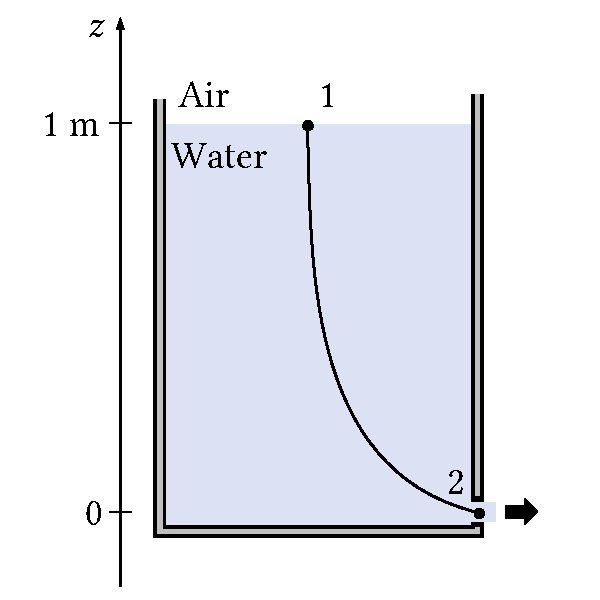
\includegraphics[width=0.5\linewidth]{Figures/Chapter3/fig_leaky_bucket}
\caption{A large tank of water has sprung a leak.  How fast is the water moving as it comes out of the hole?}
\label{fig_leaky_bucket}
\end{figure}

\begin{example}[A leaky bucket]
A large tank of water, open to the atmosphere at the top, suddenly springs a leak near the bottom (see Figure \ref{fig_leaky_bucket}).  If the hole is 1.0 m below the free surface, what is the speed of the water as it comes out the hole?

This is a good case for Bernoulli's principle, since the flow is (approximately) steady -- the surface will drop only slowly if the hole is small.  We can therefore use the streamline theorem:
\[
H = \frac{p}{\rho} + \tfrac{1}{2} \uu^2 + gz = \text{constant}.
\]
Presumably there exists a streamline that connects the free surface at the top of the tank with the hole (joining points 1 and 2 as shown in Figure \ref{fig_leaky_bucket}).  Then we can evaluate $H$ at both points:
\begin{itemize}
\item Point 1 $\to H_1 = \frac{p_1}{\rho} + \tfrac{1}{2} \uu_1^2 + gz_1$
\item Point 2 $\to H_2 = \frac{p_2}{\rho} + \tfrac{1}{2} \uu_2^2 + gz_2$
\end{itemize}
But $p_1 = p_2 = p_0$ since both locations are open to the atmosphere.  We'll also take $\uu_1 = 0$, since the surface drops only very slowly.  Finally, using the coordinate system shown in Figure \ref{fig_leaky_bucket}, we have $z_2 = 0$ (and $z_1 = 1$ m).

Setting $H_1 = H_2$ then gives us
\[
\frac{p_0}{\rho} + gz_1 = \frac{p_0}{\rho} + \tfrac{1}{2} \uu_2^2.
\]
The pressure terms cancel, and we can rearrange for the speed of the water:
\[
|\uu| = \sqrt{2gz_1} \approx 4.4 \text{ m/s}.
\]
\end{example}






\subsection{The Vorticity Equation}
\label{sec_vorticity_eq}

Let's rewrite Euler's equation again, this time in terms of the vorticity.  Going back to equation (\ref{eq_bernoulli}) and writing $\vort = \curl \uu$, we have
\[
\frac{\partial \uu}{\partial t} + \vort \times \uu = -\grad H.
\]
Take the curl of both sides:
\begin{equation}
\frac{\partial \vort}{\partial t} + \curl (\vort \times \uu) = -\curl \grad H.
\label{eq_curl_euler}
\end{equation}
But the curl of a gradient is identically zero (see Problem \ref{prob_vc2}), so the right hand side vanishes.

Now, there's a vector identity (another one!) that says, for two vectors $\symbfup{F}$ and $\symbfup{G}$,
\begin{equation}
\curl (\symbfup{F} \times \symbfup{G}) = (\symbfup{G} \cdot \grad) \symbfup{F} - (\symbfup{F} \cdot \grad) \symbfup{G} + \symbfup{F} (\symbfup{\nabla} \cdot \symbfup{G}) - \symbfup{G} (\symbfup{\nabla} \cdot \symbfup{F})
\end{equation}
(see Problem \ref{prob_vc4}).  Using this in equation \ref{eq_curl_euler} above, with $\vort$ replacing $\vec{F}$ and $\uu$ replacing $\symbfup{G}$, gives us
\[
\frac{\partial \vort}{\partial t} + (\uu \cdot \grad) \vort - (\vort \cdot \grad)\uu + \vort (\symbfup{\nabla} \cdot \uu) - \uu(\symbfup{\nabla} \cdot \vort) = 0.
\]
Of course, we're dealing with an ideal fluid, so $\symbfup{\nabla} \cdot \uu = 0$, and, since $\vort$ is a curl, $\symbfup{\nabla} \cdot \vort = 0$ identically (see Problem \ref{prob_vc2} again for that one).  So the fourth and fifth terms vanish, and we have
\[
\frac{\partial \vort}{\partial t} + (\uu \cdot \grad) \vort = (\vort \cdot \grad)\uu.
\]
Finally, we can combine the two terms on the right hand side -- that's the definition of the material derivative of $\vort$ -- and we have, at long last, the \emph{vorticity equation},
\begin{equation}
\label{eq_vorticity}
\boxed{
\frac{D \vort}{Dt} = (\vort \cdot \grad) \uu.
}
\end{equation}

This equation will prove useful every once in a while for us.  In particular, for a two dimensional flow, where 
\[
\vort = [0,0,\omega],
\]
it's easy to see that the right hand side becomes zero, and we end up with
\begin{equation}
\frac{D \vort}{Dt} = 0.
\end{equation}
This means that the vorticity of each individual fluid element is conserved, a result we'll use later.  Furthermore, if the flow is also steady, this becomes
\begin{equation}
(\uu \cdot \grad) \omega = 0,
\end{equation}
and the vorticity is constant along streamlines in this case.



\subsection{Circulation}
\label{sec_circulation}

\begin{figure}
\centering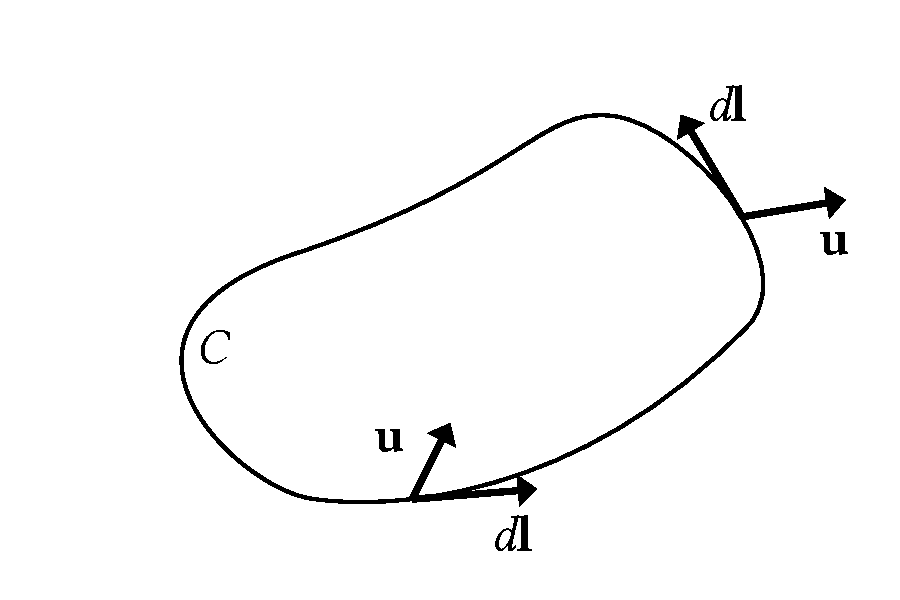
\includegraphics[width=0.5\linewidth]{Figures/Chapter3/fig_circ}
\caption{A closed curve $C$ lies within the fluid region.}
\label{fig_circ}
\end{figure}

Consider a closed curve $C$ that lies in the fluid region as shown in Figure \ref{fig_circ}.  The circulation $\Gamma$ is defined as the line integral
\begin{equation}
\boxed{
\Gamma = \oint_C \uu \cdot d\vec{l}.
}
\label{eq_circ}
\end{equation}
Notice the role the dot product plays in the integral -- as we go around the curve, only the fluid velcity that points in the direction of the curve is added, giving us the fluid that is circulating around that curve.

\begin{example}[Line Vortex]
We've explored the flow around al ine vortex before -- its vorticity in Example \ref{ex_vorticity_line_vortex} and its generation in Section \ref{sec_line_vortex} -- and we'll see it again later on.  Now let's find the circulation around it.

The flow is given by
\[
\vec{u} = \frac{\Gamma_0}{2\pi s} \, \unit{\phi},
\]
and to calculate the circulation we'll use a circular path of constant radius $R$.  The dot product in the integral becomes
\[
\vec{u} \cdot d\vec{l} = \left( \frac{\Gamma_0}{2\pi s} \, \unit{\phi} \right) \cdot \left( ds \, \unit{s} + s d\phi \, \unit{\phi} + dz \, \unit{z} \right),
\]
where we evaluate $\vec{u}$ and $d\vec{l}$ aloing the curve, and get
\[
\vec{u} \cdot d\vec{l} = \frac{\Gamma}{2\pi}.
\]
The circulation is then
\[
\Gamma = \oint_0^{2\pi} \frac{\Gamma_0}{2\pi} \, d\phi = \Gamma_0.
\]
So the line vortex has \emph{constant} circulation with strength given by $\Gamma_0$.
\end{example}

We can write the defintion of the circulation in a different way using Stokes' theorem:
\begin{equation}
\label{eq_circ_curl}
\Gamma = \oint_C \vec{u} \cdot d\vec{l} = \int_S (\grad \times \vec{u} ) \cdot d\vec{a},
\end{equation}
where $S$ is the surface inside the closed curve with area vector $d\vec{a}$.  Now, if $\grad \times \vec{u} = \vec{0}$, then $\Gamma = 0$ as well, which means that the circulation is zero inside any irrotational flow.  However, this is only true if the fluid is \emph{everywhere} irrotational; in particular, if there is an object (like a cylinder or an airplane wing, both examples we'll be doing soon), Stokes' theorem fails and it \emph{is} possible to have circulation in the fluid.

What if we suppose the closed curve actually moves with the fluid -- so that the curve always constists of the same fluid elements?  You can visualize this by prentending we put a bit of food colouring along the curve, so that as the fluid moves about and the curve changes shape, so too will the colouring -- but it will always remain a close curve.  We'll denote the curve now as $C(t)$ to indicate its dependence on time.  

Now, \emph{Kelvin's circulation theorem} says that the circulation $\Gamma$ around $C(t)$ is \emph{independent} of time -- no matter how it changes as the fluid moves, $\Gamma$ stays the same value.  This is an important theorem, especially for understanding lift, so let's go through the proof.

Start with the time derivative of the circulation,
\[
\frac{d\Gamma}{dt} = \frac{d}{dt} \left( \oint_{C(t)} \uu \cdot d\vec{l} \right),
\]
and move the derivative into the integral.  Careful though -- this is the \emph{total} time derivative, and becomes the material derivative inside:
\[
\frac{d\Gamma}{dt} = \oint_{C(t)} \frac{D\vec{u}}{Dt} \cdot d\vec{l}.
\]
But from equation (\ref{eq_euler_bern}) we can write 
\[
\frac{D\vec{u}}{Dt} = -\grad \left(\frac{p}{\rho} + \Phi \right),
\]
so
 \[
\frac{d\Gamma}{dt} = \oint_{C(t)} \grad \left.  \left(\frac{p}{\rho} + \Phi \right) \cdot d\vec{l} = - \left(\frac{p}{\rho} + \Phi \right) \right|_{C(t)}.
\]

We now have to evaluate the pressure, density, and graviational potential along the curve $C(t)$ -- but this is a closed curve and the integration takes us back to the starting point.  Since all three quantities are single-valued functions, they have the same value at the start and end of the curve -- so we get 
\begin{equation}
\frac{d\Gamma}{dt} = 0.
\end{equation}

This result is actually very general -- the fluid could be viscous and could have holes; as long as $C(t)$ moves with the fluid the circulation along it will be constant.





\subsection{The Surface of a Rotating Fluid}

Let's end this section with a classic problem involving ideal fluids: the spinning water bucket example.  In short, we'll fill a bucket with water and start rotating the bucket, letting it come to a steady state.  We solved this problem already back in Section \ref{sec_uni_rot_fluid}, where we found the steady state of the fluid was described by the velocity
\[
\uu = \Omega s \, \unit{\phi},
\]
where $\Omega$ was the angular speed of the rotating boundary -- the bucket in this case -- and the rotation was about the $z$ axis.  Converting this to Cartesian coordinates gives us
\begin{equation}
\label{eq_bucket_vel}
\uu = [-\Omega y, \Omega x, 0].
\end{equation}

Now, we \emph{found} this velocity from the Navier-Stokes equation, and viscosity is important in getting the fluid into rotation in the first place, but once steady-state has been reached, the viscosity is no longer important and the fluid can be treated as ideal.  We can thus examine the flow further using only Euler's equation rather than the full Navier-Stokes.

If you look at a good photograph of this, you'll see that the surface of the water is \emph{curved} (Figure \ref{fig_bucket}).  What is the shape of this free surface?  Well, the thing that all fluid elements along the free surface have in common is that they have the same pressure -- namely, since they're at the surface, atmospheric pressure $p_0$.  Let's find the pressure in the water, then.

\begin{figure}[t]
\centering\includegraphics[width=0.7\linewidth]{Figures/Chapter3/fig_water_bucket.jpg}
\caption{A tank of water is smoothly spun up, causing the water to ``climb'' the sides of the tank.}
\label{fig_bucket}
\end{figure}

The $x$ component of Euler's equation, with $\symbfup{g} = [0,0,-g]$, is
\[
\frac{\partial u}{\partial t} + u\frac{\partial u}{\partial x} +  v\frac{\partial u}{\partial y} + w\frac{\partial u}{\partial z} = -\frac{1}{\rho} \frac{\partial p}{\partial x}.
\]
But the flow is \emph{steady}, and $u$ doesn't depend on $x$ or $z$.  Substituting in the fluid velocity in equation (\ref{eq_bucket_vel}), this equation reduces to
\begin{equation}
\label{eq_px}
\frac{\partial p}{\partial x} = \rho \Omega^2 x.
\end{equation}
Similarly, the $v$ and $w$ equations reduce to
\begin{equation}
\label{eq_py}
\frac{\partial p}{\partial y} = \rho \Omega^2 y
\end{equation}
and
\begin{equation}
\label{eq_pz}
\frac{\partial p}{\partial z} = -\rho g.
\end{equation}

We can now integrate to find the pressure $p(x, y, z)$.  From equation (\ref{eq_px}) we get
\[
p = \tfrac{1}{2} \rho \Omega^2 x^2 + f(y, z),
\]
where the function $f(y,z)$ is there since equation (\ref{eq_px}) is a \emph{partial} derivative -- we don't just get a constant of integration, but a possible function of the other two variables.  Integrating equation (\ref{eq_py}) gives
\[
p = \tfrac{1}{2} \rho \Omega^2 y^2 + g(x, z),
\]
and integrating equation (\ref{eq_pz}) gives
\[
p = -\rho g z + h(x, y).
\]
By inspection, it's clear that the pressure must be
\[
p(x, y, z) = \tfrac{1}{2} \rho \Omega^2 (x^2 + y^2) - \rho gz + p_1,
\]
where $p_1$ is a constant -- it's the pressure at the origin where $x=y=z=0$.

That's the pressure everywhere in the water.  To find the shape of the free surface, we'll set $p = p_0$ and solve for the height $z$:
\begin{equation}
z = \frac{\Omega^2}{2g} (x^2 + y^2) + \left( \frac{p_1 - p_0}{\rho g} \right).
\end{equation}
This is a \emph{paraboloid} -- see Figure \ref{fig_bucket_para} -- and it matches the shape in the photograph in Figure \ref{fig_bucket}.

\begin{figure}
\centering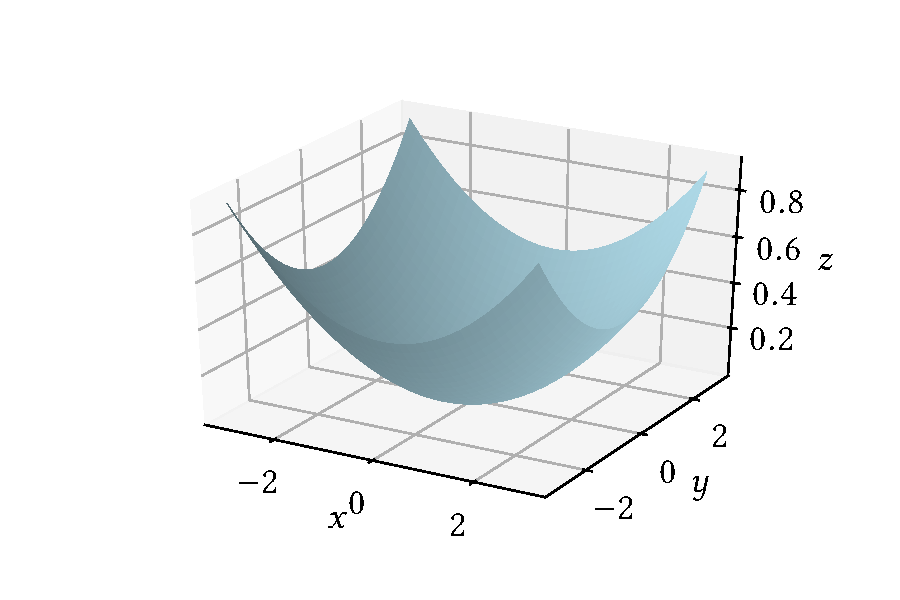
\includegraphics[width=0.8\linewidth]{Figures/Chapter3/fig_paraboloid}
\caption{The free surface of the spinning bucket problem is a paraboloid. }
\label{fig_bucket_para}
\end{figure}





\section{The Velocity Potential and Stream Function}

\subsection{The Velocity Potential}

For any irrotational flow, where
\[
\curl \uu = \vec{0},
\]
a scalar function $\varphi$ can be defined such that
\begin{equation}
\label{eq_vel_pot}
\boxed{
\uu = \grad \varphi.
}
\end{equation}
Then, since the curl of a gradient is zero, irrotationality is automatically satisfied. The quantity $\varphi$ is called the \emph{velocity potential}.  In addition, from Stokes' theorem, we also have that
\[
\oint \uu \cdot d\vec{l} = \int (\curl \uu) \cdot d\vec{a} = 0,
\]
so that the line integral of $\vec{u}$ around any closed loop in the fluid is zero.  This suggests we could also write the velocity potential as
\begin{equation}
\label{eq_vel_pot2}
\varphi(\vec{r}) = \int_{\mathcal{O}}^{\vec{r}} \uu \cdot d\symbfup{l},
\end{equation}
where $\mathcal{O}$ is an arbitrary point in the fluid.  Incidentally, sorry for the notation -- I'm using the Greek letter phi for three things:  the gravitational potential $\Phi$, the cylindrical coordinate $\phi$, and now the velocity potential $\varphi$.  I hope it's not too confusing in context.

This might be familiar to you from electrostatics, where the electric field is also irrotational and we can define an electric potential.  There's a subtle point that frequently arises in fluid dynamics, though, so be careful.  As long as the region is \emph{simply connected} -- that is, the fluid has no holes in it -- the path between $\mathcal{O}$ and $\vec{r}$ doesn't matter, and this leads to $\varphi$ being a single-valued function.  However, if the region is \emph{multiply connected} -- it has holes, regions where there is no fluid -- the integral \emph{could} depend on the path and $\varphi$ will be a multivalued function of position.  This can happen is the fluid is surrounding an object, something we'll start to encounter more frequently.  Let's investigate this in more detail with two examples.

\begin{example}[Flow past a stagnation point]
\label{ex_stag_pot}
Recall the flow past a stagnation point (from Examples \ref{ex_stag_point1} to \ref{ex_stag_point2}), given by
\[
\uu = [\alpha x, -\alpha y, 0].
\]
This is irrotational flow (but check to be sure!), and to find the velocity potential, we write
\[
\frac{\partial \varphi}{\partial x} = u = \alpha x \quad \text{and} \quad \frac{\partial \varphi}{\partial y} = v = -\alpha y.
\]
Integrating each term and combining gives
\[
\varphi(x, y) = \tfrac{1}{2} \alpha (x^2 - y^2) + c,
\]
where $c$ is the integration constant.  However, since it's the fluid velocity, not the potential, that is the physically meaningful quantity, we can set the constant $c$ to zero without losing anything -- after all, we'll take a derivative of $\varphi$ to get the velocity, and the constant will end up going anyway.

Note that, in this example, $\varphi$ is a single-valued function of $x$ and $y$.  That means that, for any point in the fluid, $\varphi$ has a single value.  This might not always be the case, as our next example will show.
\end{example}

\begin{example}[Line vortex flow]
\label{ex_pot_vortex}
Next, consider the flow
\[
\uu = \frac{\Gamma}{2\pi s} \, \hat{\phi}.
\]
This is the flow around a line vortex, which we've also seen before.  We have to be a bit more careful for this flow -- it's irrotational (we showed that back in Problem \ref{prob_vortex_vorticity}), but not at the origin where it blows up.  To fix this problem, we'll suppose there's \emph{no} fluid there -- maybe there's a cylinder of radius $a$ there instead, covering up the problem area.  That means the fluid domain is $s \ge a$, but it also means there's now a hole in the fluid domain; it's multiply connected.

The potential is found from equation (\ref{eq_vel_pot}) as usual, but in cylindrical coordinates it looks like
\[
\frac{\partial \varphi}{\partial s} = u_s = 0, \quad \frac{1}{s} \frac{\partial \varphi}{\partial \phi} = u_\phi = \frac{k}{s}, \quad \text{and} \quad \frac{\partial \varphi}{\partial z} = u_z = 0.
\]
Integrating this gives
\begin{equation}
\varphi(\phi) = k \phi.
\end{equation}
But note that this isn't a single-valued function -- $\varphi$ has different values at the same point in space:  $\varphi(0) = 0$, but $\varphi(2\pi) = 2\pi k$, and so on.  We'll see later on that this is connected to circulation within the fluid.

\end{example}

Finally, if the fluid is both irrotational \emph{and} incompressible, it must also satisfy the incompressibility condition,
\[
\symbfup{\nabla} \cdot \uu = 0.
\]
If we rewrite this in terms of the potential, we get
\[
\symbfup{\nabla} \cdot \grad \varphi = 0,
\]
or
\begin{equation}
\boxed{
\nabla^2 \varphi = 0.
}
\end{equation}
This is \emph{Laplace's equation}; any irrotational, incompressible fluid must satisfy it.





\subsection{Flow Past a Cylinder}
\label{sec_cylinder}

Working with the velocity potential rather than the velocity itself is often easier; not only is a scalar function easier to work with than a vector field, but Laplace's equation can be easier to solve than Euler's equation, which also contains the pressure of the fluid as an unknown.  As an example of solving Laplace's equation, we'll find the ideal flow past a cylinder oriented perpendicular to the flow.

We'll start with a few basic assumptions.  First, we'll treat this as two dimensional flow, which means the cylinder is effectively infinitely long.  We'll put the cylinder, which has a radius $a$, along the $z$-axis, and the flow will be uniform in the $x$-direction infinitely far away from the cylinder (see Figure \ref{fig_cyl_setup2}):
\begin{equation}
\label{eq_uniform}
\uu (\infty) = U \, \unit{x},
\end{equation}
where $U$ is the constant speed of the flow far away from the cylinder.

\begin{figure}
\centering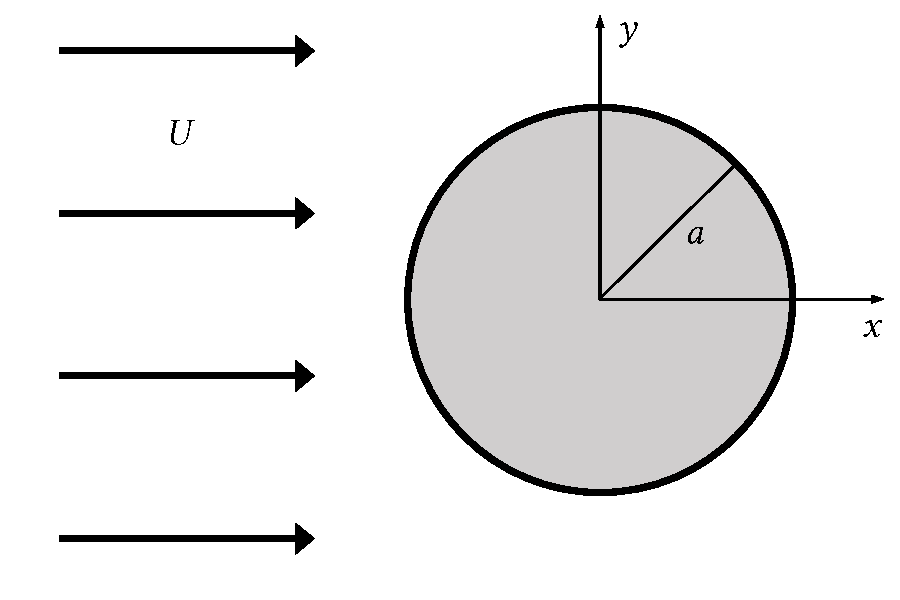
\includegraphics[width=0.7\linewidth]{Figures/Chapter3/fig_cyl_setup}
\caption{Fluid flows past the cylinder along the $x$-direction.}
\label{fig_cyl_setup2}
\end{figure}

The other assumption we'll make is that the flow is irrotational.  This seems like a leap to make, though, since we don't even know what the flow \emph{is} yet.  But remember the vorticity equation (equation \ref{eq_vorticity}) -- for a steady two dimensional flow, the vorticity is conserved along streamlines.  Since the vorticity at infinity, where the flow is \emph{uniform}, is definitely zero, and every streamline starts and ends at infinity, it follows that the flow is everywhere irrotational.

Wait, is our flow \emph{steady}?  Yes, as long as we examine the problem from the point of view that the flow has been happening for a while and reached a steady state.  In practice, it doesn't take long for the fluid to do this.

To find the fluid velocity around the cylinder, we'll solve Laplace's equation.  It makes sense to use cylindrical coordinates here, given the symmetry of the boundary.  In cylindrical coordinates, then, Laplace's equation is
\begin{equation}
\label{eq_laplace_cyl}
\ddfdx{\varphi}{s} + \frac{1}{s} \dfdx{\varphi}{s} + \frac{1}{s^2} \ddfdx{\varphi}{\phi} + \ddfdx{\varphi}{z} = 0.
\end{equation}
Of course, we're assuming a two dimensional flow, so the $z$ term we can safely ignore.

Our boundary conditions are straightforward to write down.  First, as $s \to \infty$, we should have the uniform flow given by equation (\ref{eq_uniform}).  But we need the potential rather than the velocity; following similar steps as in the examples above, the potential for uniform flow along the $x$-direction is
\begin{equation}
\label{eq_cyl_bc1}
\varphi = Ux = U s \cos \phi,
\end{equation}
where I've converted the Cartesian coordinates to cylindrical.  Our first boundary condition, then, is that the flow must become this as $s \to \infty$.

Secondly, at $s=a$, we have the actual boundary.  Unlike viscous flows, ideal fluids must ``slip'' along a boundary; in this case, that means we must have the fluid velocity at $s=a$ be purely in the $\unit{\phi}$ direction.  In other words, we need $u_s = 0$; in terms of the potential (using the gradient in cylindrical coordinates), that's
\begin{equation}
\label{eq_cyl_bc2}
\dfdx{\varphi}{s} = 0 \quad \text{at} \quad s=a.
\end{equation}

We'll solve Laplace's equation using separation of variables.  Let
\[
\varphi(s, \phi) = S(s) \Phi(\phi).
\]
Then equation (\ref{eq_laplace_cyl}) becomes
\[
\Phi \frac{d^2S}{ds^2} + \frac{\Phi}{s} \frac{dS}{ds} + \frac{S}{s^2} \frac{d^2 \Phi}{d\phi^2} = 0,
\]
or, dividing by $S\Phi$ and multiplying by $s^2$,
\begin{equation}
\label{eq_cyl_sep}
\frac{s^2}{S} \frac{d^2S}{ds^2} + \frac{s}{S} \frac{dS}{ds} = -\frac{1}{\Phi} \frac{d^2 \Phi}{d \phi^2}.
\end{equation}
The left hand side of the equation is a function of $s$ only, while the right hand side is a function of $\phi$ only; they must therefore both be equal to a constant.  We'll call the this separation constant $k^2$.  The $\phi$ equation is then
\[
\frac{d^2 \Phi}{d\phi^2} = -k^2 \Phi,
\]
which has the solution
\[
\Phi (\phi) = A \sin k\phi + B \cos k\phi.
\]

We can apply our first boundary condition, equation (\ref{eq_cyl_bc1}), right away to eliminate the sine term, since we need only a cosine dependence as $s \to \infty$.  Comparing the form of equation (\ref{eq_cyl_bc1}) with our solution, we furthermore must have $k=1$.  Thus 
\begin{equation}
\Phi(\phi) = B \cos \phi.
\end{equation}

The radial part of equation (\ref{eq_cyl_sep}) (with $k = 1$) now reads
\[
s^2 \frac{d^2S}{ds^2} + s \frac{dS}{ds} - S = 0.
\]
We've seen this differential equation before; it can solved by trying a power-law solution of the form $S(s) = s^m$.  The general solution is
\[
S(s) = Cs + \frac{D}{s}.
\]
But our second boundary condition, equation (\ref{eq_cyl_bc2}), was that the first derivative of the potential goes to zero at $s=a$.  That means
\[
\frac{dS}{ds} = \left. \left( C - \frac{D}{s^2} \right)  \right|_{s=a} = 0,
\]
and so $D = a^2 C$.

Combining the radial and angular equations gives us
\[
\varphi(s, \phi) = S(s) \Phi(\phi) = C \left( s+\frac{a^2}{s} \right) \cos \phi,
\]
where I absorbed the constants into $C$.  One more comparison with our boundary condition, equation (\ref{eq_cyl_bc1}), tells us that $C = U$.  So our solution to Laplace's equation is, finally, 
\begin{equation}
\varphi(s, \phi) = U \left( s+\frac{a^2}{s} \right) \cos \phi.
\end{equation}

That's the potential; what about the fluid velocity?  No problem:
\[
\uu = \grad \phi,
\]
so
\begin{equation}
u_s(s, \phi) = U \left( 1 - \frac{a^2}{s^2} \right) \cos \phi
\end{equation}
and
\begin{equation}
u_\phi(s, \phi) = -U \left( 1 + \frac{a^2}{s^2} \right) \sin \phi.
\end{equation}
From $\uu$, we can sketch streamlines, which are shown in Figure \ref{fig_cyl_streamlines}.

\begin{figure}
\centering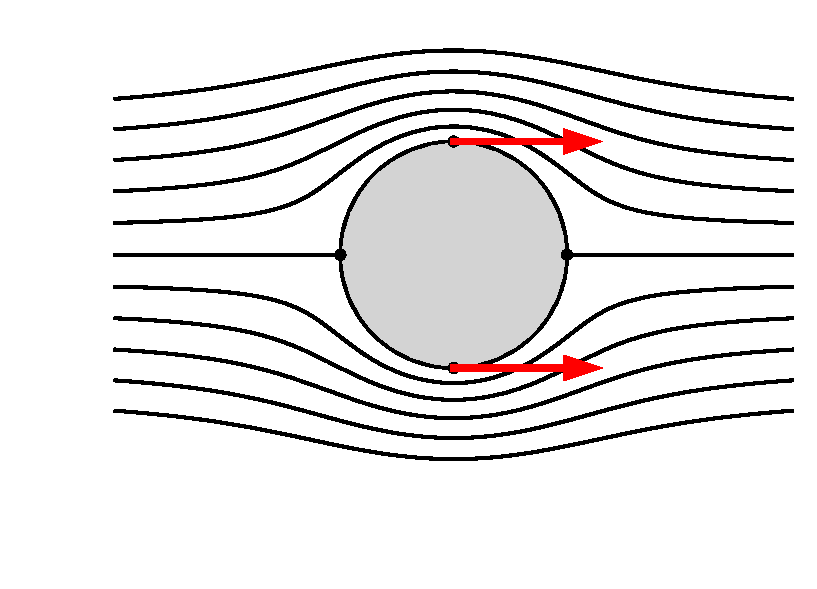
\includegraphics[width=0.7\linewidth]{Figures/Chapter3/fig_cylinder_stream}
\caption{The streamlines for the flow around the cylinder.  Note that there are stagnation points upstream and downstream of the cylinder ($\phi = 0$ and $\phi = \pi$), and the fluid has greatest velocity at the top and bottom ($\phi = \pi2$ and $\phi = 3\pi/2$).}
\label{fig_cyl_streamlines}
\end{figure}

Let's examine the flow in a little more detail.  Note that, as necessary, $u_s=0$ at $s=a$.  On the boundary, the flow is purely angular, with speed 
\[
u_\phi = -2U \sin \phi \quad \text{at} \quad s=a.
\]
At $\phi = 0$ and $\phi = \pi$, then $u_\phi = 0$ and there is a stagnation point there (see Figure \ref{fig_cyl_streamlines}).  There is a maximum speed at $\phi = \pi/2$ and $\phi = 3\pi/2$ of
\[
u_{\phi, \text{max}} = 2U \quad \text{at} \quad s=a.
\]

What about the pressure in the fluid?  Well, we could apply Euler's equation to find it, but Bernoulli's principle provides a shortcut.  Since the flow is irrotational, $\grad H = 0$ and $H = p/\rho + \tfrac{1}{2} \uu^2 + gz = $ constant everywhere in the fluid.  In our analysis, though, we'll neglect the gravity term; we're only looking at the $(s, \phi)$ dependence of the pressure here, and gravity will only impose an overall vertical pressure gradient.

Let's first evaluate $H$ at infinity, where $\uu = (U,0,0)$ and we'll label the pressure $p_\infty$.  Then
\[
H = \frac{p_\infty}{\rho} + \tfrac{1}{2} U^2.
\]
Elsewhere in the fluid, it's
\[
H = \frac{p(s, \phi)}{\rho} + \tfrac{1}{2} \uu^2,
\]
where
\[
\uu^2 = \uu \cdot \uu = u_s^2 + u_\phi^2 = U^2 \left( 1 + \frac{a^4}{s^4} - 2\frac{a^2}{s^2} \cos 2\phi \right)
\]
(that last step required some algebra to clean up, though).  Since $H$ is constant, we have
\[
\frac{p(s, \phi)}{\rho} + \tfrac{1}{2} U^2 \left( 1 + \frac{a^4}{s^4} - 2\frac{a^2}{s^2} \cos 2\phi \right) = \frac{p_\infty}{\rho} + \tfrac{1}{2} U^2.
\]
Rearranging gives the pressure,
\begin{equation}
p(s, \phi) = p_\infty + \tfrac{1}{2} \rho \frac{a^2}{s^2} U^2 \left( 2 \cos 2\phi - \frac{a^2}{s^2} \right).
\end{equation}
Figure \ref{fig_cyl_pressure} shows the pressure around the cylinder; there is a region of high pressure at $\phi = 0$ and $\phi = \pi$, with low pressure at $\phi = \pi/2$ and $\phi = 3\pi/2$.  Not surprisingly, this is opposite the fluid velocity -- expected, since Bernoulli's theorem holds here.

\begin{figure}[t]
\centering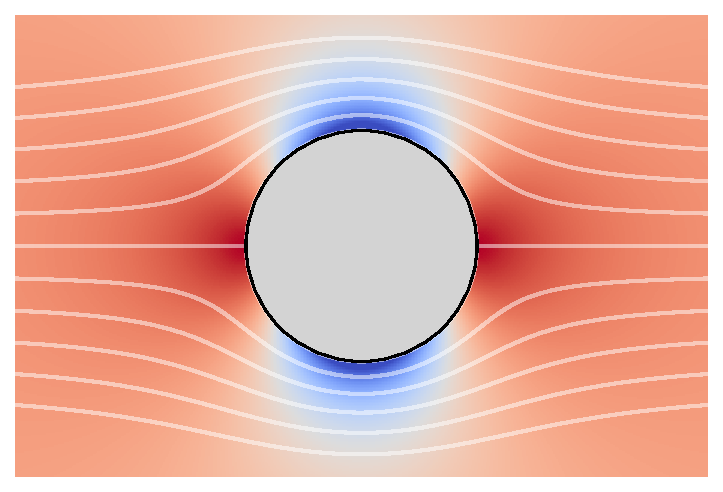
\includegraphics[width=0.8\linewidth]{Figures/Chapter3/fig_cylinder_pressure}
\caption{The pressure field of fluid flowing past a cylinder.  The dark red regions are areas of high pressure, while the blue areas are low pressure.  The streamlines are shown as well.}
\label{fig_cyl_pressure}
\end{figure}


\subsection{The Stream Function}

Let's take a break from thinking about irrotational flow for a moment, and instead consider flow that is incompressible (it's important to note that the velocity potential $\varphi$ doesn't require incompressibility to describe flow, just irrotationality).  We'll impose the further restriction that it is also two dimensional only -- so $\vec{u} = [u(x, y, t), v(x, y, t), 0]$.  In this case, we'll define the \emph{stream function} $\psi$ by
\begin{equation}
\label{eq_stream_def}
\boxed{
\vec{u} = \curl (\psi \, \unit{z}).
}
\end{equation}

Why this particular function?  Well, consider it in Cartesian coordinates,
\begin{equation}
u = \dfdx{\psi}{y} \quad \text{and} \quad v = - \dfdx{\psi}{x}.
\end{equation}
With this definition, the incompressibility equation is automatically satisfied:
\[
\grad \cdot \uu = \dfdx{u}{x} + \dfdx{v}{y} = \dfdx{}{x} \left( \dfdx{\psi}{y} \right) + \dfdx{}{y} \left( - \dfdx{\psi}{x} \right) = 0,
\]
since the order of the derivatives doesn't matter.  Compare this with the velocity potential:  it ensures irrotational flow, while the stream function ensures incompressible flow, at the cost of requiring it to be two dimensional.  By the way, in cylindrical coordinates, this definition becomes
\begin{equation}
\label{eq_stream_cyl}
u_s = \frac{1}{s} \dfdx{\psi}{\phi} \quad \text{and} \quad u_\phi = - \dfdx{\psi}{s}.
\end{equation}

You might be wondering why the stream function has that particular name -- and it turns out the reason is one of its most useful features.  Note that
\[
(\vec{u} \cdot \grad ) \psi = u\dfdx{\psi}{x} + v\dfdx{\psi}{y} = \dfdx{\psi}{y} \dfdx{\psi}{x} + \left( -\dfdx{\psi}{x} \right) \dfdx{\psi}{y} = 0.
\]
Remember what this means from Section \ref{sec_tot_deriv} -- that $\psi$ is constant on streamlines; hence the name.  If we know the stream function $\psi$, we'll now be able to easily plot the streamlines:  just set $\psi$ to a constant.  Different values of the constant will give you different streamlines.


\begin{example}[Flow past a stagnation point]
\label{ex_stag_psi}
Let's continue on from Example \ref{ex_stag_pot} and find the stream function for the flow
\[
\vec{u} = [\alpha x, -\alpha y, 0],
\]
which is incompressible (feel free to check) and obviously two dimensional.  From $u = \partial \psi / \partial y$ we get
\[
\dfdx{\psi}{y} = \alpha x,
\]
which integrates to 
\[
\psi(x, y) = \alpha x y + f(x),
\]
where $f(x)$ is some possible function of $x$.  From $v = -\partial \psi / \partial x$, we end up with something similar after integrating,
\[
\psi(x, y) = \alpha x y + g(y),
\]
where again $g(y)$ is our integration ``constant.''  Now, comparing the two equations for $\psi$, it's clear that we must have
\begin{equation}
\psi(x, y) = \alpha x y.
\end{equation}

Streamlines for this flow can be found from setting $\psi$ to a constant, which we'll call $k$:
\[
\psi = \alpha x y = k,
\]
or
\[
y = \frac{k}{\alpha x} = \frac{c}{x},
\]
where $c = k/\alpha$.  This exactly matches the equation we found back in Example \ref{ex_stag_stream} for the streamlines of a flow about a stagnation point.
\end{example}



\begin{example}[Line vortex flow]
\label{ex_vortex_psi}
For the line vortex flow, from Example \ref{ex_pot_vortex} with
\[
\uu = \frac{\Gamma}{2\pi s} \, \hat{\phi},
\]
the process to finding the stream function is similar, but we have to use cylindrical coordinates.  From equation (\ref{eq_stream_cyl}), we get
\[
u_s = 0 = \frac{1}{s} \dfdx{\psi}{\phi} \quad \text{and} \quad u_\phi = \frac{\Gamma}{2\pi s} = -\dfdx{\psi}{s}.
\]
From the first equation we just find that $\psi$ has no $\phi$ dependence, and from the second, upon integrating, we get
\[
\psi(s, \phi) = -\frac{\Gamma}{2\pi} \ln s.
\]

Once again we can find the streamlines from the stream function by setting $psi$ to a constant (call it $k$ again).  Doing so and solving for $s$ gives
\[
s = e^{-2\pi k / \Gamma} = \text{constant}.
\]
This makes sense, since we know this is circular flow -- the streamlines are circles of constant radius $s$.
\end{example}

Like the velocity potential, the stream function satisfies Laplace's equation as long as the flow is both incompressible and irrotational -- although here we need the additional constraint of two dimensional flow as well.  The proof is straightforward: start with the condition for irrotational flow, $\curl \uu = \vec{0}$, and substitute in the definition of the stream function from equation (\ref{eq_stream_def}) to get
\[
\curl [ \curl (\psi \, \unit{z}) ] = \vec{0}.
\]
But we can expand the curl of a curl as
\[
\curl [ \curl (\psi \, \unit{z}) ] = \grad [\grad \cdot (\psi \, \unit{z})] - \nabla^2 (\psi \, \unit{z}) = \vec{0},
\]
and, for two dimensional flow, the first term goes to zero, so we're left with
\begin{equation}
\boxed{
\nabla^2 \psi = 0.
}
\end{equation}
So both the velocity potential $\varphi$ and the stream function $\psi$ satisfy Laplace's equation for two dimensional, irrotational, incompressible flow.  Although not every problem in fluid dynamics satisfies these restriction, many do, and we'll exploit this in the next chapter to investigate some interesting and complex situations.




\section*{Problems}
\addcontentsline{toc}{section}{Problems}
\markright{Problems}%

\begin{problem}[Yet more vector calculus]
\label{prob_vc3}
Show that, for any vector field $\symbfup{v}$, you can write
\[
(\symbfup{v} \cdot \grad ) \symbfup{v} = (\curl \symbfup{v}) \times \symbfup{v} + \grad(\tfrac{1}{2} \symbfup{v}^2).
\]
\end{problem}

\begin{problem}[Please, no more vector calculus]
\label{prob_vc4}
Show that, for any two vector fields $\symbfup{F}$ and $\symbfup{G}$, you can write
\[
\curl (\symbfup{F} \times \symbfup{G}) = (\symbfup{G} \cdot \grad) \symbfup{F} - (\symbfup{F} \cdot \grad) \symbfup{G} + \symbfup{F} (\symbfup{\nabla} \cdot \symbfup{G}) - \symbfup{G} (\symbfup{\nabla} \cdot \symbfup{F})
\]
\end{problem}


\begin{problem}[The Rankine Vortex as a Model for Hurricanes]
A Rankine vortex is defined by the flow (in cylindrical coordinates)
\[
\symbfup{u}  = \left\{
 \begin{array}{l l}
    \Omega s \, \hat{\phi} & \quad \text{if $s < a$}\\
   \frac{\Omega a^2}{s} \, \hat{\phi} & \quad \text{if $s>a$,}
  \end{array} \right.
\]
where $\Omega$ and $a$ are constants (related to the wind speed and size of the ``core,'' respectively).  It serves as a useful model for a number of weather and atmospheric conditions, such as hurricanes, mesocyclones, and tornadoes.  

(a) Plot the wind speed as a function of distance, and calculate and plot the vorticity.

(b) To decide whether it is a useful model for hurricanes, I've provided (online) azimuthal wind speed data and vorticity data for Hurricane Katrina, which devastated New Orleans and the surrounding area in 2005.  The wind speed data has the first column as distance $s$ (in km) and the second column as azimuthal wind speed $u_\phi$ (in m/s).  The vorticity data has the first column as distance $s$ (in km) and the second column as vorticity $\omega$ (in $10^{-4}$ s$^{-1}$).

Use the Rankine vortex (RV) to model this hurricane; what values of $\Omega$ and $a$ give you the best fit?  Does the RV model the vorticity with those parameters as well?  Can you make any conclusions about how well the model does (e.g., is it better in some regions versus others?)

(c) Calculate the pressure throughout the hurricane and find the difference in pressure between r = 0 (the eye of the hurricane) and $s \to \infty$ (outside the storm).

(d) Finally, calculate the shape of the free surface (i.e., where the pressure is atmospheric). Plot the surface, and compare this with photos of Katrina -- how does it look?
\end{problem}



\begin{problem}[The force on a cylinder]
\label{prob_force1}
We've already calculated the pressure in the fluid around a cylinder in Section \ref{sec_cylinder}, so it's a short leap to find the total force exerted on the cylinder by the fluid.

Consider Figure \ref{fig_cylinder_force}:  the force (per unit length of the cylinder) on a small angular section of size $a \, d\phi$ is
\[
d\textbf{F} = - p \hat{n}.
\]
Using this, show the total force on the cylinder is zero.  This is called \emph{D'Alembert's paradox} -- there's no drag on the cylinder, despite very obvious physical evidence to the contrary.  Does it make sense that the fluid exerts no force at all on the cylinder as it flows past?  Discuss.

\begin{figure}[t]
\centering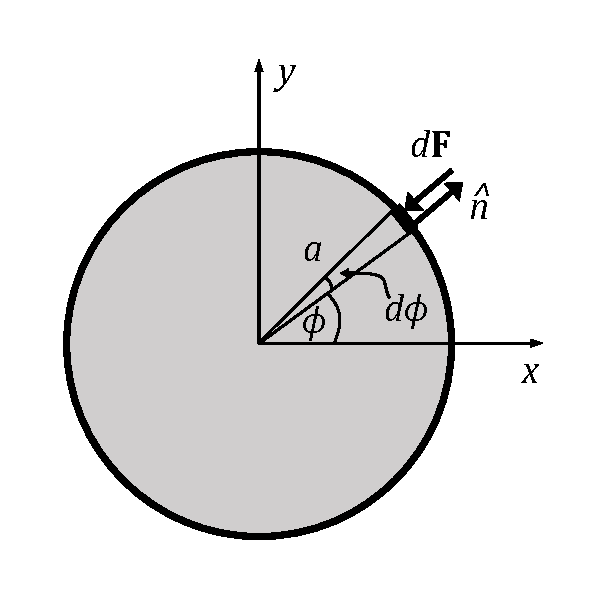
\includegraphics[width=0.5\linewidth]{Figures/Chapter3/fig_cyl_force}
\caption{The force on a small angular section of the cylinder.  The force is opposite the normal vector $\hat{n}$.}
\label{fig_cylinder_force}
\end{figure}
\end{problem}


\begin{problem}[Uniform Flow]
\label{prob_uniform_pot}
Consider two dimensional flow that is constant and flows in a direction at an angle $\alpha$ with respect to the $x$ axis (see Figure \ref{fig_uniform_flow_angle}).  

(a) Find the velocity potential $\varphi(x, y)$.

(b) Find the stream function $\psi(x, y)$.

\begin{figure}[t]
\centering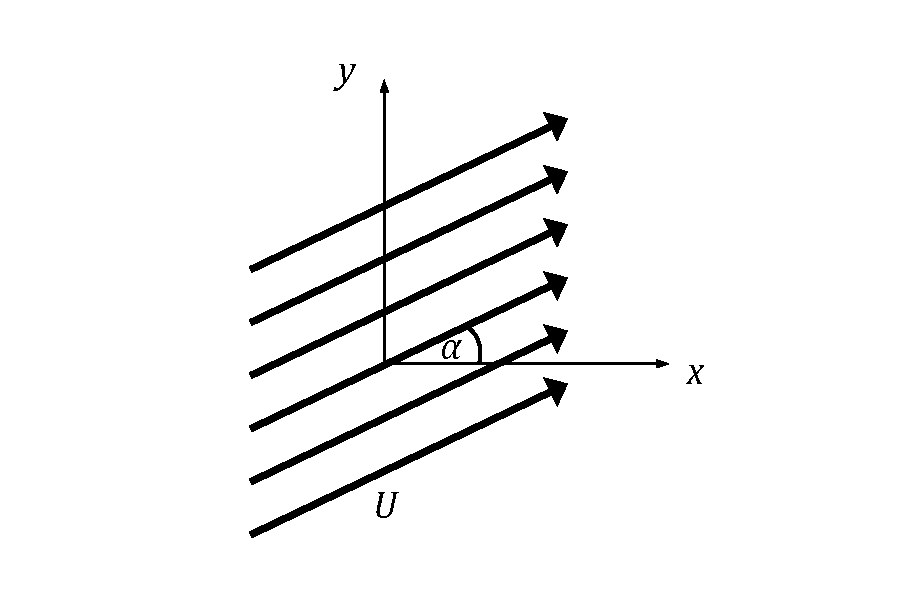
\includegraphics[width=0.7\linewidth]{Figures/Chapter3/fig_uniform_flow_angle}
\caption{A constant flow that makes an angle $\alpha$ with the $x$ axis.}
\label{fig_uniform_flow_angle}
\end{figure}
\end{problem}

\begin{problem}[Line source and sink]
\label{prob_line_source}
Consider the two dimensional flow 
\begin{equation}
\uu = \frac{Q}{2\pi s} \, \unit{s},
\end{equation}
where $Q$ is a constant (you might want to compare the form of this flow to the line vortex).  This is called a \emph{line source} if $Q$ is positive and a \emph{line sink} if it's negative.

(a) Produce a vector plot for the flow.

(b) Find the  velocity potential $\varphi(s, \phi)$.

(b) Find the stream function $\psi(s, \phi)$.
\end{problem}

\begin{problem}[Plotting streamlines]
Consider the two dimensional flow
\[
\uu = [2x+3, -2y].
\]

(a) Show that the flow is irrotational and incompressible.

(b) Find the stream function $\psi(x, y)$ and plot the streamlines.
\end{problem}


\chapter{Potential Flow}

%
%  SECTION 4.1 - THE COMPLEX POTENTIAL
%

\section{The Complex Potential}

In the previous chapter, we saw that an irrotational fluid can be described by the \emph{velocity potential} $\varphi$, defined by
\begin{equation}
\vec{u} = \grad \varphi.
\end{equation}
If, instead, the fluid is both two dimensional and incompressible, it can be described by the stream function, $\psi$, defined via
\begin{equation}
\vec{u} = \grad \times (\psi \, \unit{z}).
\end{equation}
Now, if we have a two dimensional fluid that is both irrotational \emph{and} incompressible, then we can use either $\varphi$ \emph{or} $\psi$ to describe it; in Cartesian coordinates, we have
\begin{equation}
\label{eq_u_phi_psi}
u = \dfdx{\varphi}{x} = \dfdx{\psi}{y} \quad \text{and} \quad v = \dfdx{\varphi}{y} = - \dfdx{\psi}{x}.
\end{equation}

For reasons we'll learn as we go, it's very convenient to define a \emph{third} function, the \emph{complex potential} $w(z)$:
\begin{equation}
\label{eq_complex_pot}
\boxed{
w(z) = \varphi + i \psi.
}
\end{equation}
Unlike the velocity potential and the stream function, the complex potential is a function of a \emph{single} variable -- the complex number $z$.   That makes now a good time to review our knowledge of the complex plane. 

% SECTION 4.1.1 - THE COMPLEX PLANE

\subsection{The Complex Plane}

Consider a complex number $z$:
\begin{equation}
z = x + iy.
\end{equation}
We call $x$ the \emph{real part} of the complex number and $y$ the \emph{imaginary part}.  This can be represented on a Cartesian coordinate system as shown in Figure \ref{fig_complex_plane}; the $x$ axis is the real axis and the $y$ axis the imaginary.  This is called the \emph{complex plane}. 

\begin{figure}
\centering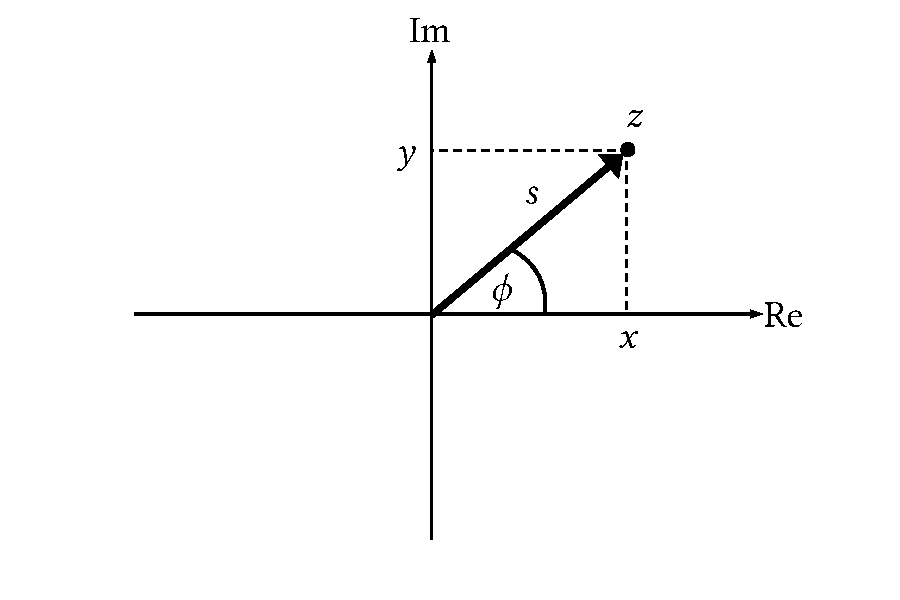
\includegraphics[width=0.7\linewidth]{Figures/Chapter4/fig_complex_plane}
\caption{The complex plane showing the complex number $z = x + iy = s \, e^{i\phi}$.}
\label{fig_complex_plane}
\end{figure}

In addition to using Cartesian coordinates, we can also write the complex number $z$ in polar coordinates; it should be clear from the figure that
\[
z = x + iy = s \cos \phi + is \sin \phi.
\]
Using Euler's famous formula,
\[
e^{i \phi} = \cos \phi + i \sin \phi,
\]
this becomes
\begin{equation}
z = s \, e^{i \phi}.
\end{equation}

Some operations, like multiplying complex numbers, are easier in polar coordinates.  Other operations are unique to complex numbers, such as taking the \emph{complex conjugate} of $z$; this means that every imaginary number $i$ becomes the negative $-i$.  The complex conjugate is denoted with a star:
\[
z^* = x - iy = s \, e^{-i\phi}.
\] 
Although we can square a complex number as normal,
\begin{equation}
\label{eq_z_squared}
z^2 = (x + iy)^2 = x^2 - y^2 + 2ixy,
\end{equation}
an operation that often comes up is the ``complex square,''
\begin{equation}
|z|^2 \equiv z^* z = (x-iy)(x+iy) = x^2 + y^2.
\end{equation}
Notice that the complex square will always give a real number.

Sometimes you'll have a complex number in the denominator of a fraction, which makes it difficult to separate the real and imaginary parts of the complex number -- something we'll do pretty frequently.  You can always get rid of the imaginary part in the denominator by multiplying by the complex conjugate:
\[
\frac{1}{x + iy} = \frac{1}{x+iy} \frac{x - iy}{x-iy} = \frac{x - iy}{x^2 + y^2}.
\]

So far, this is all pretty basic stuff, but we need at least one thing from the more advanced theory of complex analysis -- we'll be working with \emph{complex functions} $f(z)$.  Like complex numbers, complex functions can be separated into real and imaginary parts,
\[
f(z) = f(x + iy) = A(x, y) + i B(x, y),
\]
where $A(x, y)$ and $B(x, y)$ are real-valued functions.  Now, a complex function is \emph{analytic} if $A$ and $B$ are differentiable and satisfy the so-called \emph{Cauchy-Riemann conditions,}
\begin{equation}
\label{eq_cauchy_riemann}
\dfdx{A}{x} = \dfdx{B}{y} \quad \text{and} \quad \dfdx{A}{y} = - \dfdx{B}{x}.
\end{equation}
This means that the complex derivative exists, and can be written as\footnote{This is obviously a drastically shortened and simplified look at complex analysis; for more, see e.g., \emph{Mathematical Method for Physicists}, 4th edition, by Arfken and Weber, Chapter 6.}
\begin{equation}
\frac{df}{dz} = \dfdx{A}{x} + i \dfdx{B}{x} = \dfdx{B}{y} - i \dfdx{A}{y}.
\end{equation}

You might have noticed that the Cauchy-Riemann conditions look a lot like equation (\ref{eq_u_phi_psi}) -- the relationship between the velocity potential and the stream function.  This is the connection to fluid dynamics:  by construction, the complex potential $w(z)$ is an analytic complex function, which means we can write the derivative of it as
\begin{equation}
\label{eq_w_deriv}
\boxed{
\frac{dw}{dz} = \dfdx{\varphi}{x} + i \dfdx{\psi}{x} = u - iv.
}
\end{equation}
Thus the derivative of the complex potential is related to the speed of the fluid by
\[
|\vec{u} | = \left| \frac{dw}{dz} \right| = \sqrt{ \left( \frac{dw}{dz} \right)^* \left( \frac{dw}{dz} \right) }.
\]
This gives us a powerful tool to examine some pretty complicated flows.


% SECTION 4.1.2- BASIC FLOWS

\subsection{Basic Flows}

Although we're restricted to two dimensional, incompressible, irrotational flows, the complex potential is nonetheless a useful description of fluid flow in a variety of cases.  We'll start here with four basic flows, and will build up to fluid flow around a wing of an airplane, all the while using tools of complex analysis.

\begin{figure}
\centering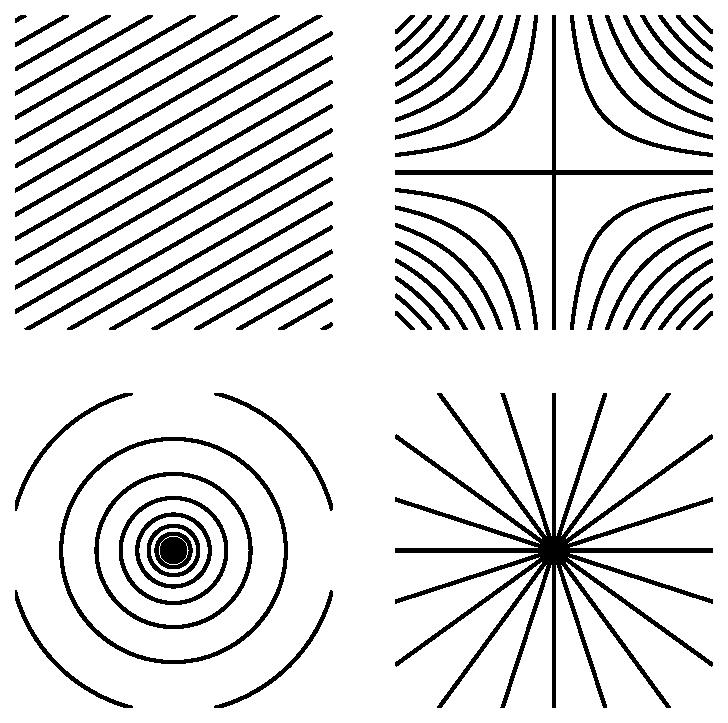
\includegraphics[width=0.6\linewidth]{Figures/Chapter4/fig_basic_flows}
\caption{Four basic potential flows.  Upper left: uniform flow at an angle $\alpha$.  Upper right: flow about a stagnation point.  Lower left: a line vortex.  Lower right: a line source.}
\label{fig_basic_flows}
\end{figure}

\begin{example}[Uniform flow]
To start, consider a simple flow that is uniform everywhere.  We'll suppose it flows at an angle $\alpha$ with the $x$ axis, so that the velocity is
\begin{equation}
\vec{u} = [U\cos \alpha, U\sin \alpha, 0].
\end{equation}
Problem \ref{prob_uniform_pot} asked you to work out the details, but the velocity potential in this case is
\begin{equation}
\varphi (x, y) = U(x \cos\alpha + y\sin\alpha)
\end{equation}
and the stream function is
\begin{equation}
\psi (x, y) = U(y \cos\alpha - x\sin\alpha).
\end{equation}

To find the complex potential, we'll start with equation (\ref{eq_complex_pot}) to get
\[
w = \varphi + i\psi = U(x \cos\alpha + y\sin\alpha) + iU(y \cos\alpha - x\sin\alpha).
\]
We can simplify this with a bit of rearranging:
\[
w = U \left[ (x+iy) \cos\alpha - i(x+iy) \sin\alpha \right].
\]
But $z = x+iy$ so we have
\[
w = Uz(\cos\alpha - i\sin\alpha),
\]
or, using Euler's formula,
\begin{equation}
w(z) = Uze^{-i\alpha}.
\end{equation}
This is the complex potential for uniform flow at an angle $\alpha$.  Note that is is a function only of $z$ -- all the $x$s and $y$s have disappeared, which is necessary for the complex potential.
\end{example}

\begin{example}[Stagnation point flow]
Let's return to a flow we've studied plenty already, the flow about a stagnation point,
\[
\vec{u} = [\alpha x, -\alpha y, 0].
\]
In Example \ref{ex_stag_pot} we found that the velocity potential was
\[
\varphi (x, y) = \frac{1}{2} \alpha (x^2 - y^2),
\]
and in Example \ref{ex_stag_psi} we found the stream function,
\[
\psi(x, y) = \alpha xy.
\]

The complex potential for this flow is
\[
\begin{split}
w & = \varphi + i\psi = \frac{1}{2} \alpha (x^2 - y^2) + i\alpha xy \\
& = \frac{1}{2} \alpha ( x^2 - y^2 + 2ixy ).
\end{split}
\]
If this doesn't look familiar, take a look at equation (\ref{eq_z_squared}) -- the term in the brackets is just $z^2$, so the complex potential is
\begin{equation}
w(z) = \frac{1}{2} \alpha z^2.
\end{equation}

\end{example}


\begin{example}[A line vortex]
\label{ex_line_vortex_w}
Another familiar flow is the line vortex, covered in Examples \ref{ex_pot_vortex} and \ref{ex_vortex_psi}.  For reference, the velocity for this flow is
\[
\vec{u} = \frac{\Gamma}{2\pi s} \, \unit{\phi},
\]
and the velocity potential and stream function are
\[
\varphi(s, \phi) = \frac{\Gamma \phi}{2\pi} \quad \text{and} \quad \psi(s, \phi) = -\frac{\Gamma}{2\pi} \ln s.
\]
We'll construct the complex potential in the same way as above, but we'll have to use polar coordinates to build the complex number $z$.  We have
\[
w = \frac{\Gamma \phi}{2\pi}  -i\frac{\Gamma}{2\pi} \ln s
\]
and can pull out a factor of $-i\Gamma / 2 \pi$ to get
\[
w = -\frac{i\Gamma}{2\pi} \left( i\phi + \ln s \right).
\]
Now we'll have to use a bit of a trick:  we can write $i\phi$ as
\[
i\phi = \ln \left( e^{i\phi} \right),
\]
and then combine the two natural logarithms to get
\[
w = -\frac{i\Gamma}{2\pi} \ln \left( s e^{i\phi} \right).
\]
But in polar coordinates, $z = s e^{i\phi}$, so we finally have
\begin{equation}
w(z) = -\frac{i\Gamma}{2\pi} \ln z.
\end{equation}

\end{example}

\begin{example}[A line source]
For our final example, consider the flow about a \emph{line source},
\begin{equation}
\vec{u} = \frac{Q}{2\pi s} \, \unit{s},
\end{equation}
where $Q$ is a constant.  Problem \ref{prob_line_source} has some more information, but the velocity potential is
\begin{equation}
\varphi (s, \phi) = \frac{Q}{2\pi} \ln s,
\end{equation}
while the stream function is
\begin{equation}
\psi(s, \phi) = \frac{Q \phi}{2\pi}.
\end{equation}

The complex potential for this flow is
\begin{equation}
w(z) = \frac{Q}{2\pi} \ln z,
\end{equation}
and you can work out the details yourself in Problem \ref{prob_line_source_w}.
\end{example}

These four basic flows are shown in Figure \ref{fig_basic_flows} and summarized in Table \ref{tab_pot_flows}; we'll be working with them a lot.  However, one of the powerful things about the complex potential is that they can \emph{add together}.  This is possible because, since both $\varphi$ and $\psi$ are solutions to Laplace's equation, so too is the complex potential $w = \varphi + i\psi$.  And since the Laplacian is a linear operator, any combination of solutions is a solution as well.

\begin{table}[t]
\caption{Four basic potential flows.}
\centering
  \begin{tabular}{l|l|l}
  Flow & Velocity & Complex Potential \\ \hline
  Uniform flow & $\vec{u} = [U\cos \alpha, U\sin \alpha]$ &  $w(z) = Uz e^{-i\alpha}$ \\
  Stagnation point & $\vec{u} = [\alpha x, -\alpha y]$ &  $w(z) = \frac{1}{2} \alpha z^2$ \\
  Line vortex & $\vec{u} = \frac{\Gamma}{2\pi s} \unit{\phi}$ & $w(z) = -\frac{i\Gamma}{2\pi} \ln z $ \\
  Line source & $\vec{u} = \frac{Q}{2\pi s} \unit{s}$ & $w(z) = \frac{Q}{2\pi} \ln z$
  \end{tabular}
  
  \label{tab_pot_flows}
\end{table}


For example, suppose we combine a line source with a uniform flow (with angle $\alpha = 0$):
\[
w(z) = Uz + \frac{Q}{2\pi} \ln z.
\]
This complex potential is a perfectly valid description of \emph{some} fluid flow -- it's incompressible and irrotational and satisfies Laplace's equation.  Now, whether or not this is flow that we actually \emph{see} is up to experiment to test; in this case the flow represents fluid around an object called a \emph{Rankine half body}.

We can investigate this flow further by finding the stream function and plotting streamlines.  Remember that $\psi$ is the imaginary part of the complex potential,
\[
\psi = \operatorname{Im}(w).
\]
Finding the imaginary part isn't always simple for a general complex potential, although in this case it's not difficult and you should try it on your own.  I'll discuss this a bit more in the next section; for now, the streamlines are plotted in Figure \ref{fig_uniform_source}.  It's not difficult to imagine how a flow like this might arise -- the red streamline could be the boundary of an object in the fluid, and the flow is passing this object.  This is because for ideal fluids the fluid must ``slip'' along a boundary (there's no no-slip condition for ideal fluids), meaning the boundary must be a streamline.  This boundary condition will play an important role in our next example.

\begin{figure}
\centering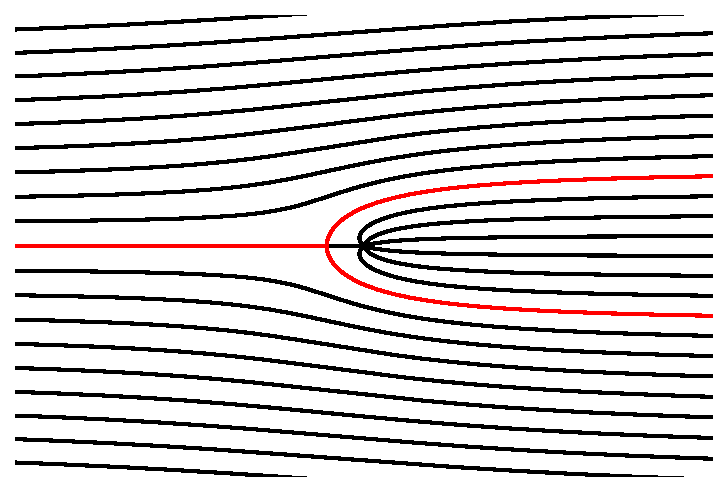
\includegraphics[width=0.7\linewidth]{Figures/Chapter4/fig_uniform_source}
\caption{Streamlines for a flow that includes both uniform flow and a line source.}
\label{fig_uniform_source}
\end{figure}


% SECTION 4.1.3 - METHOD OF IMAGES

\subsection{Method of Images}
\label{sec_images}

Consider a single line vortex, but we'll modify the flow in two ways:  first, by moving it to a new position $z_0 = d$ along the $x$ axis, and secondly by putting a wall at $x=0$, effectively having the fluid in the domain $x>0$ only.  This is shown in Figure \ref{fig_mirror_wall}.  Now, the first adjustment is easy to make, since moving the line vortex location just means shifting the origin in the opposite direction; in general, a line vortex at a location $z_0 = x_0 + iy_0$ in the complex plane is given by
\begin{equation}
\label{eq_line_vortex_z0}
w(z) = -\frac{i\Gamma}{2\pi} \ln (z-z_0).
\end{equation}

\begin{figure}
\centering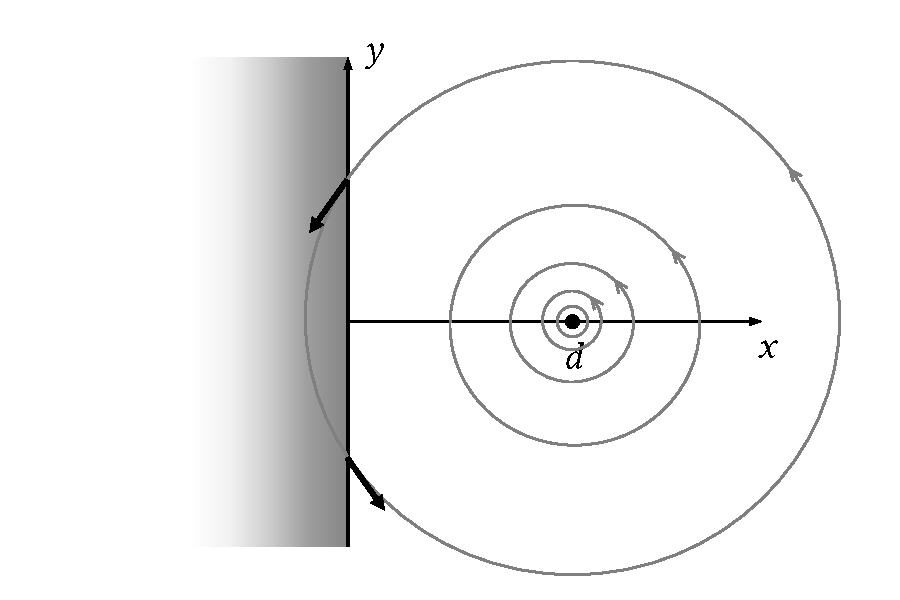
\includegraphics[width=0.75\linewidth]{Figures/Chapter4/fig_mirror_wall}
\caption{A line vortex a distance $d$ from a wall.}
\label{fig_mirror_wall}
\end{figure}

What about the wall?  That's a little trickier, since it's apparent that the flow given in equation (\ref{eq_line_vortex_z0}) doesn't satisfy the boundary conditions -- we need the flow to slip along the wall.  That means we require our flow at $x=0$ to be along the $y$ direction only, so that
\[
u(0, y) = 0.
\]
As shown in Figure  \ref{fig_mirror_wall}, the flow is tangent to the streamlines, and doesn't point just along $y$ at the wall.  In fact, it looks like the fluid is either flowing \emph{into} the wall or \emph{out of} the wall, which doesn't make much sense physically.  How can we adjust our complex potential to satisfy the boundary condition?

Well, never mind for a moment.  Instead, consider a completely \emph{different} problem:  two vortexes, one at $z = d$ as above, and one at $z = -d$; there's no wall in this problem.  The second vortex will have the same strength as the first, but will go in the opposite direction:  $\Gamma_2 = - \Gamma_1$; see Figure \ref{fig_mirror_image}.  Since complex potentials add together, it's simple to write down $w(z)$ for this new flow:
\[
w(z) = -\frac{i\Gamma}{2\pi} \ln (z-d) + \frac{i\Gamma}{2\pi} \ln (z+d)
\]
(notice the plus sign -- the second term is for the vortex that rotates in the opposite sense as the first).  We can simplify this a bit using log rules to get
\begin{equation}
\label{eq_mirror_vortex}
w(z) = -\frac{i\Gamma}{2\pi} \ln \left( \frac{z - d}{z+d} \right).
\end{equation}

Now, \emph{this} flow \emph{does} satisfy the boundary condition -- the two flows from each vortex combine at the wall and the $x$ components of the velocity end up cancelling, giving components along the $y$ direction only.  In other words, this flow slips along the boundary; you can prove this mathematically if you want by trying Problem \ref{prob_mirror_bc}.

\begin{figure}
\centering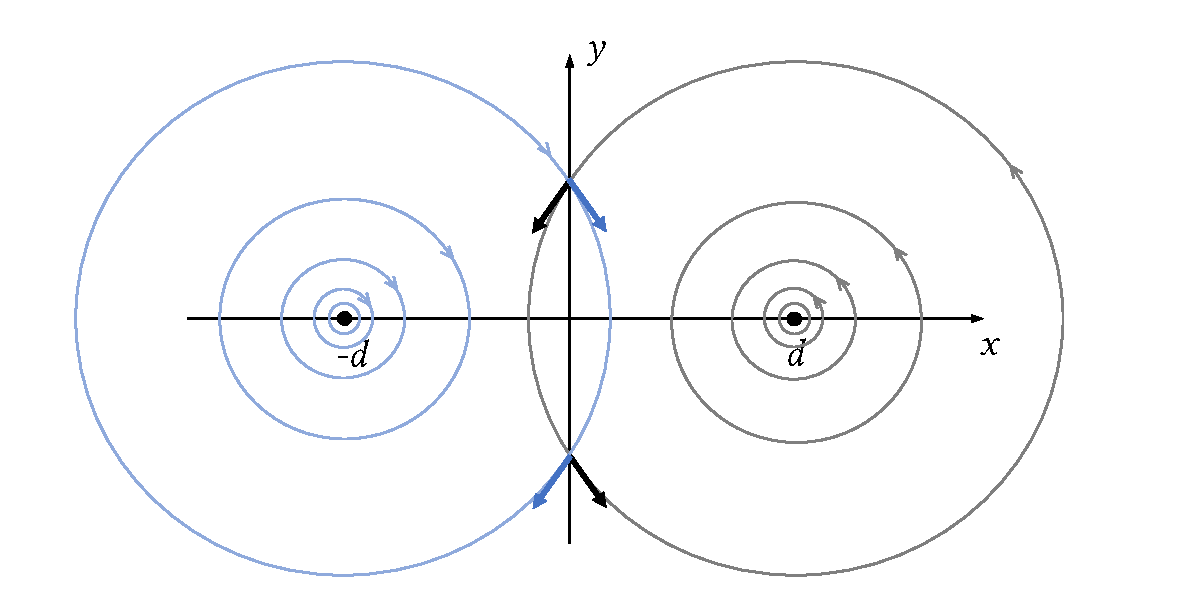
\includegraphics[width=\linewidth]{Figures/Chapter4/fig_mirror_image}
\caption{Two line vortexes combine to create a flow that slips along the wall.}
\label{fig_mirror_image}
\end{figure}

By adding a second vortex, we've satisfied the boundary conditions of the original problem; this is a technique called method of images, which you might know from electrostatics.  Of course, in the original problem, we had only \emph{one} vortex, not two -- but that's okay, since our second vortex is covered up by the wall.  It's not really there, and our solution is only good for the domain $x>0$.  

Method of images works because our fluid satisfies Laplace's equation, and solutions to Laplace's equation are \emph{unique}: if a complex potential is a solution to Laplace's equation \emph{and} satisfies the boundary conditions of the problem, then it's \emph{the} solution.\footnote{Griffiths has an excellent discussion of uniqueness theorems and Laplace's equation in \emph{Introduction to Electrodynamics}, 4th edition, Chapter 3; as usual there's much more to say about the matter.}

One more thing before we move on.  What does the flow in $x>0$ actually look like?  Figure \ref{fig_mirror_image} gives streamlines for each vortex superimposed, not combined properly.  To find the streamlines, we need the stream function,
\[
\psi = \operatorname{Im}(w).
\]
As I mentioned above, it's not always easy to find the imaginary part of the complex potential, particularly when logarithms are involved.  I'll walk you through a general method for doing so, and we'll start with the polar form of the complex number $z$:
\[
z = s e^{i\phi}.
\]
Here, $s$ is often called the \emph{modulus}, and is the complex absolute value of $z$,
\[
s = |z| = \sqrt{z^*z},
\]
and $\phi$ is called the argument.  Now, if we just have the logarithm of a complex number, that's easy enough to split into real and imaginary parts, and we've already seen the reverse of it in Example \ref{ex_line_vortex_w}:
\[
\ln z = \ln s + i\phi.
\]
Note that the real part of $\ln z$ is the logarithm of the modulus $s$ and the imaginary part is the argument $\phi$.  Careful, though -- in fact, I could add a multiple of $2\pi$ to $\phi$ and still get the same $\ln z$, so there's actually an infinite number of possibilities for the imaginary part of $\ln z$.  Writing it as I did means $\ln z$ is called the \emph{principle value.} This is something we won't have to worry about much, but I wanted to mention it for completeness. 

If we have something more complicated, say the logarithm of a complex function $f(z)$, the idea is the same,
\[
\ln \left[ f(z) \right] = \ln \left| f(z) \right| + i \operatorname{Arg} \left[ f(z) \right].
\]

Now, it might not be simple to find the argument of the function $f(z)$ -- you'll have to split it into its real and imaginary parts, 
\[
f(z) = A(x, y) + iB(x, y),
\]
and then find the argument from
\[
\operatorname{Arg}\left[ f(z) \right] = \operatorname{Arg}\left[ A(x, y) + iB(x, y) \right] = \tan^{-1} \left[ \frac{B(x,y)}{A(x,y)} \right].
\]
Things can once again get complicated in dealing with the arctan function, but luckily we won't have to worry about this much either.  The modulus at least is normally not a problem, since
\begin{equation}
\left| f(z) \right| = \sqrt{ f^*(z) f(z) }.
\end{equation}

In the case of the vortex beside the wall, we can now write
\[
w(z) = -\frac{i\Gamma}{2\pi} \ln \left( \frac{z - d}{z+d} \right) = -\frac{i\Gamma}{2\pi} \left[ \ln \left| \frac{z-d}{z+d} \right| + i \operatorname{Arg} \left( \frac{z-d}{z+d} \right) \right]
\]
or
\[
w(z) = \frac{\Gamma}{2\pi}\operatorname{Arg} \left( \frac{z-d}{z+d} \right) - i \frac{\Gamma}{2\pi} \ln \left| \frac{z - d}{z+d} \right|,
\]
and we can identify the stream function as the imaginary part,
\begin{equation}
\psi(x, y) = \frac{\Gamma}{2\pi} \ln \left| \frac{z - d}{z+d} \right|.
\end{equation}
Careful, though -- there are still complex numbers $z$ in that equation for $\psi$, which should be a real function.  However, because the complex absolute value is there, it's guaranteed to be real -- if you work it out (it's a bit of algebra but not too hard), you get
\begin{equation}
\psi(x, y) = -\frac{\Gamma}{2\pi} \ln \sqrt{ \frac{x^2 + y^2 - 2xd + d^2}{x^2 + y^2 + 2xd + d^2} }.
\end{equation}
From the stream function you can plot the streamlines of the flow as shown in Figure \ref{fig_vortex_wall}; notice that one streamline lies directly along the wall.

\begin{figure}
\centering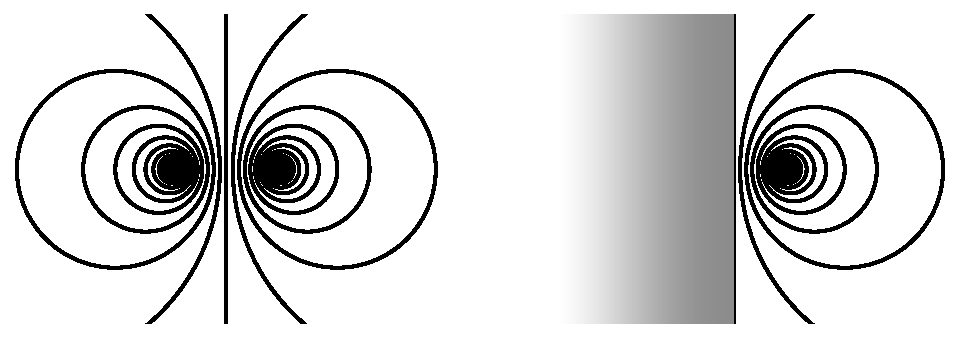
\includegraphics[width=0.9\linewidth]{Figures/Chapter4/fig_vortex_wall}
\caption{The streamlines for a line vortex a distance $d$ from a wall.  The left side shows both vortexes, while the right side shows just the real vortex beside the wall.}
\label{fig_vortex_wall}
\end{figure}


% SECTION 4.1.4 - THE CIRCLE THEOREM

\subsection{The Circle Theorem}

Take a close look at Figure \ref{fig_vortex_wall} -- although the circular streamlines are no longer \emph{concentric}, they are still circular.  That suggests that this complex potential can also work for a line vortex within a \emph{circular} boundary (say, a cylindrical bucket filled with fluid) -- as long as the boundary matches one of the streamlines, our boundary condition will be satisfied and the fluid will slip along the circular wall.

Consider the situation shown in Figure \ref{fig_circular_boundary}.  We'll put the origin of our coordinate system at the centre of the cylindrical bucket (of radius $a$) and orient the $x$ axis so that the line vortex of strength $\Gamma$ is located on it at $x = c_1$.  To ensure a streamline matches the boundary of the cylinder, we'll need a mirror image of the vortex (with opposite circulation $-\Gamma$) on the $x$ axis -- outside the cylinder.  The question is \emph{where} do we put it?

\begin{figure}
\centering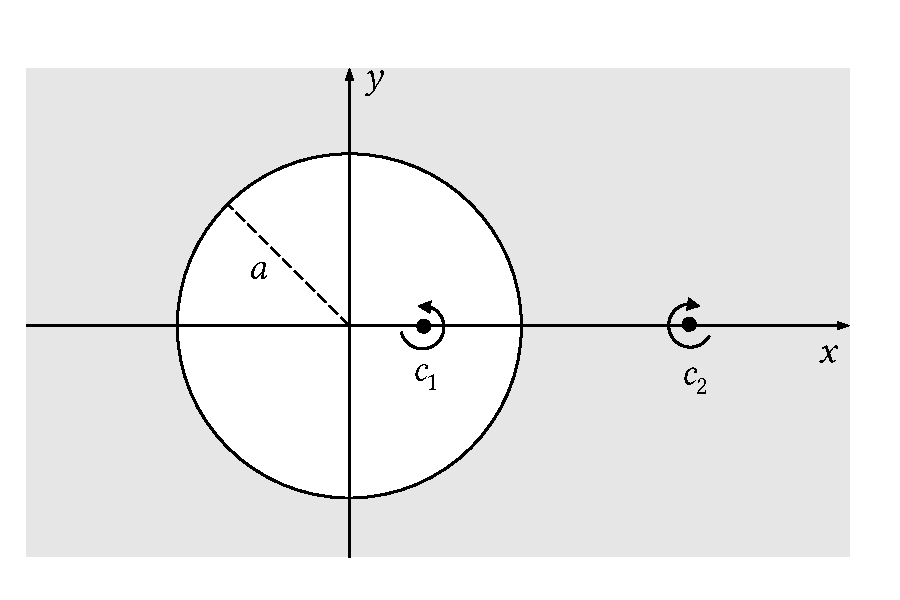
\includegraphics[width=0.75\linewidth]{Figures/Chapter4/fig_circular_boundary}
\caption{A line vortex in a circular bucket can be modelled with a mirror image outside the bucket.}
\label{fig_circular_boundary}
\end{figure}

Take a look at the circles on the left side of Figure \ref{fig_vortex_wall} again -- they're a well-known system called \emph{coaxal circles}.  The members of a coaxal system are described by the equation
\begin{equation}
\label{eq_coaxal_circles}
x^2 + y^2 + 2\lambda x + k = 0,
\end{equation}
with different values of $\lambda$ giving different circles.  These two sets of circles have \emph{limiting points} at $x = \pm \sqrt{k}$ -- that's where they converge to a circle of radius zero.  In our problem here, the positions of the two line vortexes at $x=c_1$ and $x=c_2$ would be the limiting points. From equation (\ref{eq_coaxal_circles}) you can derive a relationship between the radius $a$ of one of the circles and the two limiting points; it turns out to be
\[
a^2 = c_1 c_2.
\]
If we have a vortex at $x=c_1$ inside the cylinder, placing a mirror vortex at 
\begin{equation}
c_2 = \frac{a^2}{c_1}
\end{equation}
will give streamlines that match the boundary.  The complex potential of a vortex in a cylindrical bucket a distance $c$ from the centre is therefore
\begin{equation}
w(z) = -\frac{i\Gamma}{2\pi} \ln (z-c) + \frac{i\Gamma}{2\pi} \ln (z-a^2/c)
\end{equation}
(I've dropped the subscript ``1'' from $c$ since we don't need $c_2$ anymore), and the streamlines are shown in Figure \ref{fig_vortex_cylinder}.

%\begin{figure}
%\centering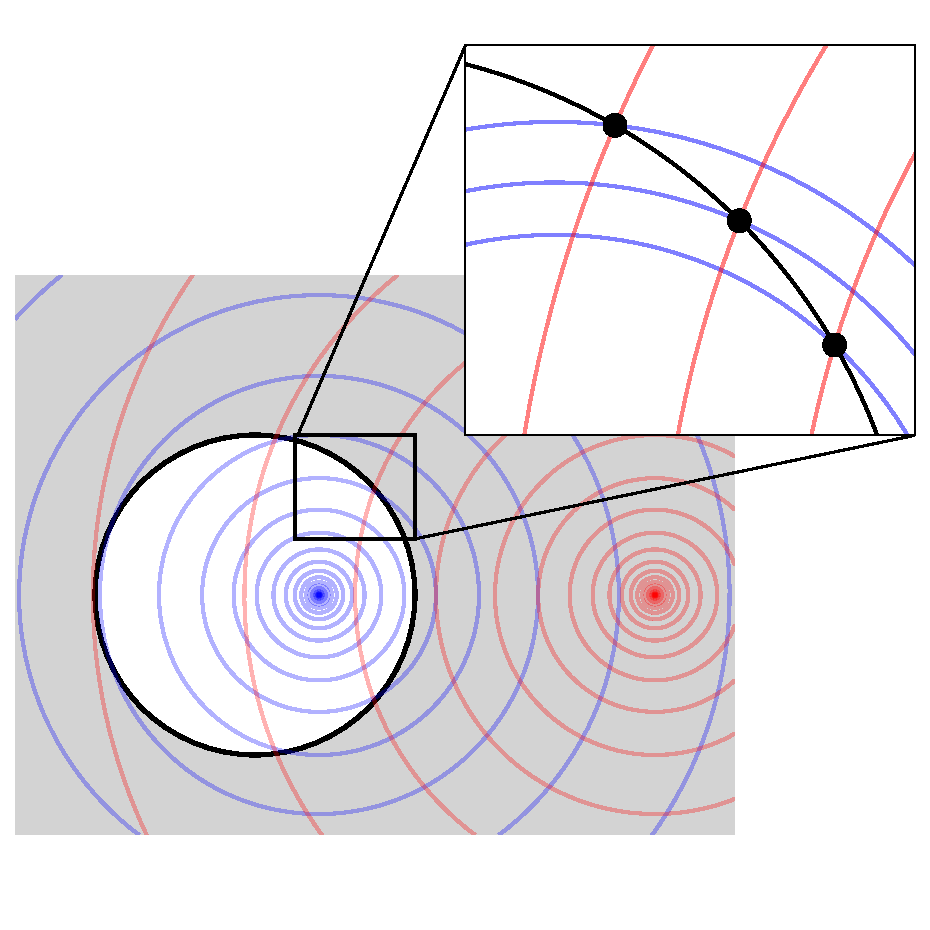
\includegraphics[width=0.75\linewidth]{Figures/Chapter4/fig_circular_inset}
%\caption{The streamlines of the two vortexes combine to give a streamlines that exactly matches the cylinder.}
%\label{fig_circular_inset}
%\end{figure}

\begin{figure}
\centering
\includegraphics[width=0.5\linewidth]{Figures/Chapter4/fig_vortex_cylinder}
\caption{The streamlines of a line vortex within a circular cylinder.}
\label{fig_vortex_cylinder}
\end{figure}

The idea of placing a vortex in a flow to get a circular streamline is very general -- and powerful.  The Milne-Thompson Circle Theorem gives us a way to add a circular streamline to any irrotational, incompressible flow, and is given by the following:
\begin{theorem}[Milne-Thompson Circle Theorem]
Consider a flow described by the complex potential
\[
w = f(z),
\]
and any singularities of $f(z)$ (in other words, where it goes to infinity) occur in the region $|z| > a$.  Then the new complex potential
\begin{equation}
w = f(z) + f^*(a^2 / z^*)
\end{equation}
describes a flow that has the same singularities as $f(z)$ in $|z| > a$ \emph{and} has the circle $|z| = a$ as a streamline.
\end{theorem}

This is straightforward to prove.  The circle $|z| = a$ can be written as
\[
|z|^2 = z^* z = a^2,
\]
or
\[
z^* = \frac{a^2}{z}.
\]
That means that, on the circle itself,
\[
w = f(z) + f^*(a^2/z^*) = f(z) + f^*(z).
\]
But the function $f(z) + f^*(z)$ is a \emph{real} function; suppose we write $f(z) = A(x, y) + iB(x, y)$, in which case it's easy to see that 
\[
f(z) + f^*(z) = A(x, y) + iB(x,y) + A(x, y) - iB(x, y) = 2A(x, y),
\]
and the imaginary part has cancelled. If $w(z)$ is a \emph{real} function on the circle, then it's imaginary component must be zero:
\[
\psi(x, y) = \operatorname{Im}(w) = 0.
\]
Never mind the zero -- the important thing is to see that $\psi$ is \emph{constant} along the circle.  That means the circle is a streamline!

What about the singularity part?  Well, any point that is originally outside the circle in $f(z)$ actually ends up \emph{inside} the circle in $f^*(a^2/z^*)$, so no new singularities outside $|z| = a$ are created -- that means the new flow has the same singularities as the original flow.

%
% SECTION 4.2 - FLOW PAST OBJECTS
%

\section{Flow Past Objects}



% SECTION 4.2.1 - FLOW PAST A CYLINDER

\subsection{Flow Past a Cylinder}

As a simple example of the Circle Theorem, consider starting with uniform flow with angle $\alpha = 0$, given by
\[
w(z) = Uz.
\]
Using the Circle Theorem we get
\[
w(z) = Uz + \left[ U \frac{a^2}{z^*} \right]^*
\]
or
\begin{equation}
w(z) = U \left( z + \frac{a^2}{z} \right).
\end{equation}
This is the complex potential for a flow that is uniform at infinity but has a circular streamline centred at the origin with radius $a$; see Figure \ref{fig_uniform_circle}. The streamlines outside the circular streamline might look familiar if you recall Section \ref{sec_cylinder}, and we'll examine them closely in a moment.  But what about the streamlines interior to the circle?  They're similar to the streamlines for a \emph{doublet} flow, in which $w \propto z^{-1}$, but that doesn't really matter -- in fact, if we ``cover up'' the fluid interior to $|z| = a$ with, say, a circular cylinder, then what we've done is find the complex potential for flow around that cylinder.

\begin{figure}
\centering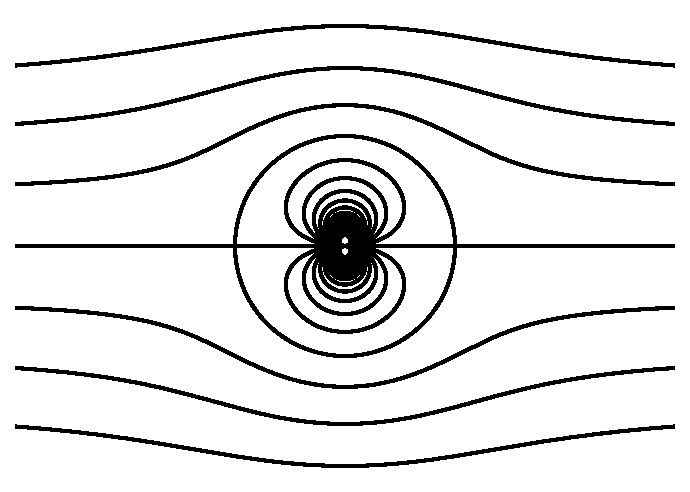
\includegraphics[width=0.7\linewidth]{Figures/Chapter4/fig_uniform_circle}
\caption{The streamlines for the flow generated by applying the Circle Theorem to a uniform flow.}
\label{fig_uniform_circle}
\end{figure}

Does our solution match the one we found earlier in Section \ref{sec_cylinder}?  We can find the velocity potential and stream function easily enough (see Problem \ref{prob_circlular_cylinder}); they are
\begin{equation}
\varphi(s, \phi) = U \left( s + \frac{a^2}{s} \right) \cos\phi
\end{equation}
and
\begin{equation}
\psi(s, \phi) = U \left( s - \frac{a^2}{s} \right) \sin\phi.
\end{equation}
We can also find the velocity of the flow, either from the potential or stream function, or from the derivative of the complex potential directly using equation (\ref{eq_w_deriv}); either way, we get
\begin{equation}
u_s(s, \phi) = U \left( 1 - \frac{a^2}{s^2} \right) \cos\phi
\end{equation}
and
\begin{equation}
u_\phi(s, \phi) = U \left( 1 + \frac{a^2}{s^2} \right) \sin\phi.
\end{equation}
These do indeed match the flow we found earlier -- by much more laborious means (solving Laplace's equation).  It's hard to overstate just how powerful the Circle Theorem can be; we found in a few lines what took us four pages of solving a partial differential equation before.

But we can do more in this case.  It's trivial to add an angle $\alpha$ to the uniform flow, for example; in that case we start with the complex potential
\[
w(z) = Uz e^{-i\alpha}
\]
and get, using the Circle Theorem,
\begin{equation}
w(z) = U \left( ze^{-i\alpha} + \frac{a^2}{z}e^{i\alpha} \right).
\end{equation}
We could also add a line vortex, placed at the origin, to our flow.  This wouldn't change the fact that there's a circular streamline at $|z| = a$, since the line vortex has circular streamlines, but would change the flow $u_\phi$ at the surface of the cylinder -- in effect, we're adding \emph{circulation} to the flow, as we'll see.  Remember, complex potentials add together, so the flow with a line vortex is simply
\begin{equation}
\label{eq_uniform_circle}
w(z) = U \left( ze^{-i\alpha} + \frac{a^2}{z}e^{i\alpha} \right) - \frac{i\Gamma}{2\pi} \ln z.
\end{equation}

\begin{figure}
\centering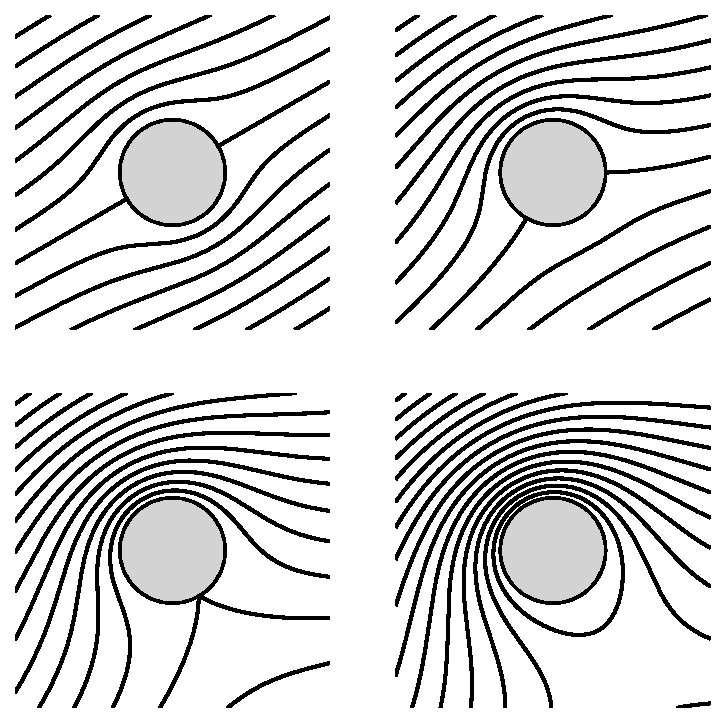
\includegraphics[width=0.75\linewidth]{Figures/Chapter4/fig_cylinder_circ}
\caption{Streamlines for flow around a circular cylinder at an angle $\alpha = \pi/6$.  Upper left: circulation $\Gamma = 0$.  Upper right: circulation $\Gamma = -2\pi Ua$.  Lower left: circulation $\Gamma = -4\pi Ua$.  Lower right: circulation $\Gamma = -6\pi Ua$.}
\label{fig_cylinder_circ}
\end{figure}

Streamlines with circulation in the flow are shown in Figure \ref{fig_cylinder_circ}.  Something interesting happens as the circulation $\Gamma$ increases:  notice that the two stagnation points, normally at opposite ends of the cylinder, come closer together as the circulation increases, until 
\[
\Gamma = \pm 4\pi U a,
\]
when they combine to form just one stagnation point.  If the circulation is greater than this, they disappear completely -- we now have fluid circulating completely around the cylinder, as you can see by the streamlines in the lower right part of Figure \ref{fig_cylinder_circ} (note that the circulation is negative in the Figure, so that the fluid circulates clockwise around the cylinder; we'll see why I chose this shortly).  You can explore this flow more in Problem \ref{prob_circlular_cylinder}.

Back in Problem \ref{prob_force1} you may have calculated the force of the fluid on a circular cylinder for flow without circulation -- it turned out to be zero, a somewhat surprising result called d'Alembert's paradox.  Because we're dealing with ideal fluids and the flow is symmetric, the fluid is unable to push on the cylinder.  However, this result changes when circulation is added to the flow.  Problem \ref{prob_force2} can walk you through the details of the calculation, but nothing changes for the $x$ component of force -- the fluid still doesn't push on the cylinder in the direction of the oncoming flow -- but there \emph{is} a force in the $y$ direction, perpendicular to the uniform flow:
\begin{equation}
\label{eq_force1}
F_y = -\rho U \Gamma.
\end{equation}
This force is due entirely to the circulation around the cylinder, and if $\Gamma$ is negative, as the examples in Figure \ref{fig_cylinder_circ} show, then the force is upward:  the fluid provides \emph{lift} on the cylinder.  Of course, the wings of an airplane aren't at all circular in cross section, but this essential idea -- that circulation around the object is necessary for lift -- will return when we discuss proper aerofoils.



% SECTION 4.2.2 - CONFORMAL MAPPING

\subsection{Conformal Mapping}

Suppose we have some general complex potential $w(z) = \varphi + i\psi$.  Our goal is to create a \emph{mapping} or \emph{transformation} between the complex plane $z = x+iy$ and a second complex plane, which I'll write with capital letters: $Z = X + iY$.  We'll perform this transformation with the function $f(z)$ such that
\begin{equation}
Z = f(z).
\end{equation}
We'll assume $f(z)$ is an \emph{analytic} complex function, meaning it's differentiable, and that it has an inverse given by
\begin{equation}
z = F(Z)
\end{equation}
(and $F(Z)$ is also an analytic function).

The complex potential is transformed as well -- in the $Z$ complex plane it takes on the form
\begin{equation}
W(Z) = w[F(Z)].
\end{equation}
Now, we can split $W(Z)$ into it's real and imaginary parts,
\begin{equation}
W(Z) = \Phi(X, Y) + i\Psi(X, Y).
\end{equation}
Here's the amazing thing:  because $W$ will be an analytic function of $Z$, $\Phi$ and $\Psi$ will satisfy the Cauchy-Riemann conditions (equation \ref{eq_cauchy_riemann}), and therefore
\begin{equation}
\U(X, Y) = \dfdx{\Phi}{X} = \dfdx{\Psi}{Y} \quad \text{and} \quad \V(X, Y) = \dfdx{\Phi}{Y} = -\dfdx{\Psi}{X}
\end{equation}
represent a possible fluid flow -- that is, the velocity  $\U \, \unit{X} +  \V \, \unit{Y}$ is an irrotational, incompressible flow that satisfies Laplace's equation.

This might seem like a lot to take in at first, but our goal is to use a transformation to map our flow around a circular cylinder to other possible shapes -- including, eventually, a realistic wing shape.  Before we get there, though, let's take a look at a simple example.



\begin{example}[A Simple Conformal Map]
\label{ex_conformal_map}
Consider the map
\[
Z = f(z) = \frac{z^2}{5} + 2,
\]
which has the inverse 
\[
z = F(Z) = \sqrt{5(Z-2)}.
\]
We'll start with the complex potential for uniform flow, $w(z) = Uz$; the left side of Figure \ref{fig_conformal_map} shows the streamlines (blue) as well as lines of constant velocity potential (red).  For uniform flow, these lines are straight and meet at right angles.

Under the map, the complex potential in the $Z$ complex plane becomes
\[
W(Z) = w[F(Z)] = U\sqrt{5(Z-2)};
\]
streamlines for this transformed complex potential are shown on the right panel of Figure \ref{fig_conformal_map}.  The original streamlines are mapped to new streamlines (and similarly for the lines of constant $\varphi$), and are no longer straight -- but notice that they do still cross at right angles.  This is why the mapping is called conformal -- the transformation preserves local angles.

Suppose we look at just one point in the $z$ complex plane, say
\[
z_0 = 1 + i.
\]
The complex potential at that point is $w(z_0) = U(1+i)$.  In the $Z$ complex plane, $z_0$ is mapped to
\[
Z_0 = \frac{2i}{5} + 2,
\]
but the complex potential $W(Z_0)$ has the same value as $w(z_0)$:
\[
W(Z_0) = U\sqrt{5(2i/5 + 2 - 2)} = U\sqrt{2i} = U(1+i).
\]

\end{example}

\begin{figure}
\centering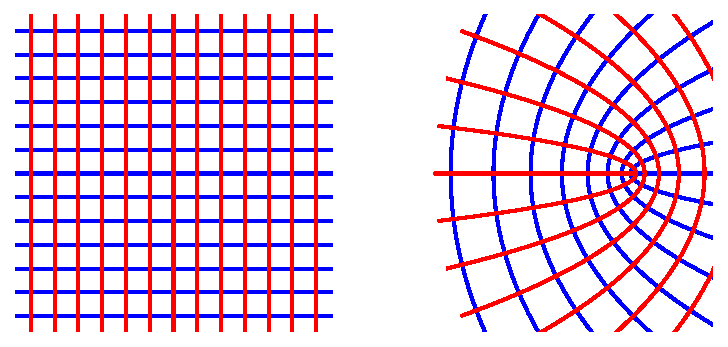
\includegraphics[width=0.75\linewidth]{Figures/Chapter4/fig_conformal_map}
\caption{The effect of the conformal map $f(z) = z^2/5 + 2$ on uniform flow.  The blue lines are the streamlines $\psi = $ constant and the red lines are lines of constant velocity potential $\varphi$.  Left: the original uniform flow, $w(z) = Uz$, in the $z$ complex plane.  Right: the flow under the conformal map $W(Z)$ in the $Z$ complex plane.}
\label{fig_conformal_map}
\end{figure}


When choosing a particular map, there are two things to be careful about.  First, consider the derivative of $W(Z)$.  Writing it as $W(Z) = w(z)$ where $z = F(Z)$, we can use the chain rule to get
\[
\frac{dW}{dZ} = \frac{dw}{dz}\frac{dz}{dZ}.
\]
But recall that $dw/dz = u - iv$, so this says
\begin{equation}
\label{eq_UV}
\U - i\V = \frac{u - iv}{dZ/dz} = \frac{u - iv}{f'(z)},
\end{equation}
using $Z = f(z)$.  If we want the streamlines in the new $Z$ complex plane to match the original streamlines in the $z$ plane at infinity -- far away from the object the fluid is flowing past -- then we'll need
\begin{equation}
f'(z) \to 1 \quad \text{as} \quad |Z| \to \infty.
\end{equation}

The second thing is about the conformal nature of the map.  Normally, local angles are preserved, as we saw in Example \ref{ex_conformal_map}.  However, this is only true if the mapping function $f(z)$ has a non-vanishing first derivative everywhere.  At points where the first derivative is zero, though, the angle changes; in general, the local angle is multiplied by $n$, where $n$ is the order of the first non-vanishing derivative of $f(z)$.  


% SECTION 4.2.4 - FLOW PAST AN ELLIPTICAL CYLINDER

\subsection{Flow Past an Elliptical Cylinder}

Let's try the following transformation:
\begin{equation}
Z = f(z) = z + \frac{c^2}{z},
\end{equation}
where $c$ is a constant.  This is called the \emph{Joukowski transformation}, and was important in the development of the theory of aerodynamics.  Note that the derivative is
\[
f'(z) = 1 - \frac{c^2}{z^2},
\]
so $f'(z) \to 1$ as $|z| \to \infty$; this mapping won't affect the flow far away from the object.  Also note that the first derivative is non-zero almost everywhere, so local angles will be preserved.  However, something interesting happens at $z = \pm c$ -- at that point the first derivative becomes zero, and the first non-vanishing derivative is the \emph{second}.  This means at those points local angles will be \emph{doubled}.

We'll need the inverse of the Joukowski transformation as well; it is given by
\begin{equation}
\label{eq_inverse_jt}
z = \frac{1}{2}Z \pm \sqrt{\frac{1}{4} Z^2 - c^2}.
\end{equation}
Note that, except at the points $Z = \pm 2c$, this inverse is \emph{multivalued}.  In the language of complex analysis, we would say that $Z = \pm 2c$ are \emph{branch points}, and we could cut the plane between them to ensure the inverse is single-valued.  However, in practice, we'll only need the positive root; it turns out that the negative root maps points in the $Z$ complex plane to points within a circle of radius $c$ on the $z$ complex plane, while the positive root maps them to points outside that circle.  Since we're studying fluid flow around objects, there won't be any fluid within that radius anyway -- the object itself will be there.

\begin{figure}
\centering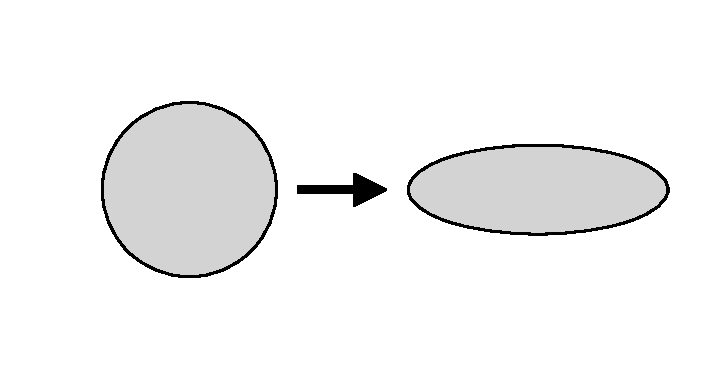
\includegraphics[width=0.75\linewidth]{Figures/Chapter4/fig_jt_ellipse}
\caption{The Joukowski transformation takes a circle in the $z$ complex place to an ellipse in the $Z$ complex plane.  Here the parameter $c = 0.7$.}
\label{fig_jt_ellipse}
\end{figure}

What does the Joulowski transform actually do?  Consider its affect on a circle of radius $a$ in the complex $z$ plane, which is given by
\[
z = a e^{i\phi}.
\]
Applying the transformation leads to 
\[
Z = z + \frac{c^2}{z} = ae^{i\phi} + \frac{c^2}{a} e^{-i\phi}.
\]
This might not look familiar, but with a bit of work we can see what it describes.  Write $Z = X + iY$ and $e^{i\phi} = \cos\phi + i\sin\phi$ and separate $Z$ into its real and imaginary components:
\[
X + iY = \left( a + \frac{c^2}{a} \right) \cos \phi + i \left( a - \frac{c^2}{a} \right) \sin \phi.
\]
Now take the complex conjugate of both sides and rearrange to get
\begin{equation}
\label{eq_ellipse}
\frac{X^2}{(a + c^2/a)^2} + \frac{Y^2}{(a - c^2/a)^2} = 1.
\end{equation}
This is the equation of an ellipse with semimajor axis $a + c^2/a$ and semiminor axis $a - c^2/a$. The shape of the ellipse is controlled by the parameter $c$, so that as $c \to a$, the ellipse gets flatter and flatter.  Figure \ref{fig_jt_ellipse} shows this Joukowski transformation.

To see what the flow around the ellipse looks like, we start with the flow around a circular cylinder of radius $a$ -- including the angle and circulation, as given by equation (\ref{eq_uniform_circle}) -- and use the inverse Joukowski transformation (equation \ref{eq_inverse_jt}) to replace all the $z$s with $Z$s. After a bit of rearranging, the complex potential around an elliptical cylinder is given by
\begin{multline}
\label{eq_ellipse_w}
W(Z) = Ue^{-i\alpha} \left( \frac{1}{2} Z + \sqrt{\frac{1}{4} Z^2 - c^2} \right) + Ue^{i\alpha} \frac{a^2}{c^2} \left( \frac{1}{2} Z - \sqrt{\frac{1}{4} Z^2 - c^2} \right) - \\ \frac{i\Gamma}{2\pi} \ln \left( \frac{1}{2} Z + \sqrt{\frac{1}{4} Z^2 - c^2} \right)
\end{multline}
To find the streamlines we have to extract the imaginary part of this very complicated complex potential.  Although possible, I'll leave it as an exercise for you to try; the streamlines themselves are shown in Figure \ref{fig_ellipse}. Luckily, producing the streamline plot with a computer is much easier than finding the streamlines by hand.

\begin{figure}
\centering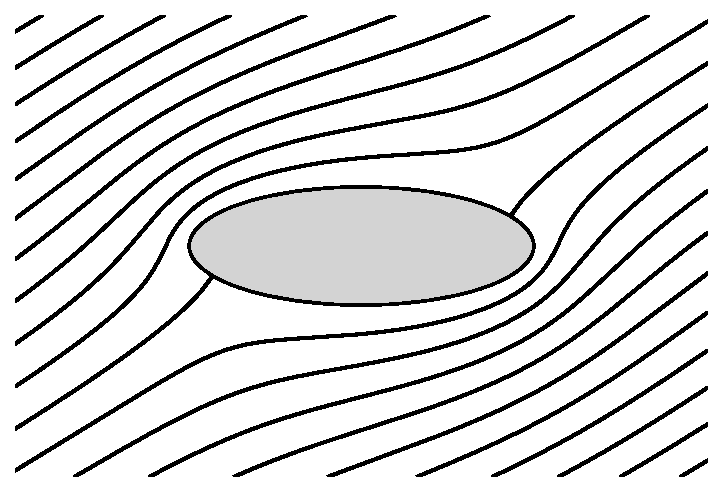
\includegraphics[width=0.7\linewidth]{Figures/Chapter4/fig_ellipse}
\caption{The streamlines for flow around an elliptical cylinder, with $c=0.7$, $\alpha = \pi/6$, and $\Gamma= 0$.}
\label{fig_ellipse}
\end{figure}


% SECTION 4.2.5 - FLOW PAST A FLAT PLATE

\subsection{Flow Past a Flat Plate}

The shape of the ellipse is dependent on the parameter $c$ in the Joukowski transformation, and if we let $c \to a$, so that the transformation is
\begin{equation}
Z = z + \frac{a^2}{z},
\end{equation}
the ellipse collapses to a flat plate.  Looking at equation (\ref{eq_ellipse}), we see that the semiminor axis goes to zero, while the semimajor axis becomes $2a$ -- so the plate has a total length of $4a$.  The flow in this case is shown in the left panel of Figure \ref{fig_flat_plate}.

Although it's difficult to see in that streamline plot, there are two points in the flow where the velocity goes to infinity -- there are two \emph{singularities}.  They occur at each edge of the plate, at $Z = \pm 2a$.  To investigate the velocity of the flow, we have to find the derivative $dW/dZ$, which can be lengthy and complicated.  To simplify things for a bit, suppose $\Gamma = 0$; letting $a=c$ in equation (\ref{eq_ellipse_w}) and taking the derivative, we get (with some simplification)
\[
\U - i\V = \frac{dW}{dZ} = U\cos \alpha - i \frac{U \sin \alpha \, Z}{\sqrt{Z^2 - 4a^2}}.
\]
You can see in the imaginary term that the denominator goes to zero as $Z \to \pm 2a$ -- so the $Y$ component of the velocity blows up there and we have a singularity in the flow.

\begin{figure}
\centering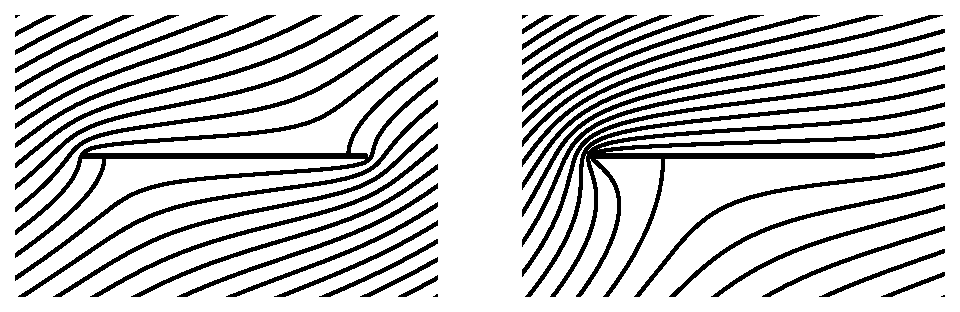
\includegraphics[width=\linewidth]{Figures/Chapter4/fig_flat_plate}
\caption{The streamlines for flow around a flat plate with angle $\alpha = \pi/6$.  Left: $\Gamma = 0$.  Right: $\Gamma= -4\pi Ua \sin\alpha$.}
\label{fig_flat_plate}
\end{figure}

Now, a singularity is not physical, so presumably in a real fluid flowing past a thin flat plate they would not exist.  One way to remove them is to set $\alpha = 0$, but that's not very general.  We can do better, but we need to resort to a bit of a trick to analyze this situation.  If we include the circulation term in equation (\ref{eq_ellipse_w}), the derivative gets even messier, so let's use equation (\ref{eq_UV}) to find the velocity components $\U$ and $\V$:
\begin{equation}
\label{eq_dwdz}
\U - i\V = \frac{dW}{dZ} = \frac{dw/dz}{f'(z)} = \frac{Ue^{-i\alpha} - U(a^2/z^2) e^{i\alpha} - i\Gamma/2\pi z}{1 - a^2/z^2}.
\end{equation}
Notice that the velocity goes to infinity at $z = \pm a$, which corresponds in the $Z$ complex plane to $Z = \pm 2a$ as we just found.  At this point, we should use the inverse Joukowski transformation, equation (\ref{eq_inverse_jt}), to replace all the $z$s with $Z$s, but it's not necessary as long as we're careful.

If you look at the velocity, you might notice that we can remove \emph{one} singularity from the flow by choosing just the right amount of circulation:  if 
\begin{equation}
\Gamma = -4\pi Ua \sin \alpha,
\end{equation}
then the numerator of equation (\ref{eq_dwdz}) goes to zero at $z = +a$ along with the denominator.  You can show that, in this case, the flow remains finite at $z = a$ and becomes (see Problem \ref{prob_flat_plate})
\begin{equation}
\U = U\cos\alpha \quad \text{and} \quad \V = 0 \quad \text{at} \quad Z = 2a.
\end{equation}
The flow with this choice is shown in the right hand panel of Figure \ref{fig_flat_plate}. We've removed the singularity at the right edge of the plate -- called the \emph{trailing edge} -- with an astute choice of circulation, but the singularity still exists at the \emph{leading edge}.  To fix that one, we'll have to do one more clever trick.




% SECTION 4.2.6 - FLOW PAST AN AEROFOIL

\subsection{Flow Past an Aerofoil}

The trick is simple -- we're going to hide the leading edge singularity \emph{inside} the object, where there is no fluid.  To do that, we'll shift the circle in the $z$ complex plane to the left by an amount $\lambda$; see the left panel of Figure \ref{fig_aerofoil} for how this looks. Note that we still want the circle to extend to $z=+a$ on the right side, so we'll also increase the radius of the circle to $a + \lambda$.  Even if $\lambda$ is a small value, $z=-a$ will be covered by the circle, and when transformed to the $Z$ complex plane, the point $Z = -2a$ will be covered by the object the circle is transformed into under the Joukowski transformation -- a classic aerofoil shape, as shown in the right panel of Figure \ref{fig_aerofoil}.

\begin{figure}
\centering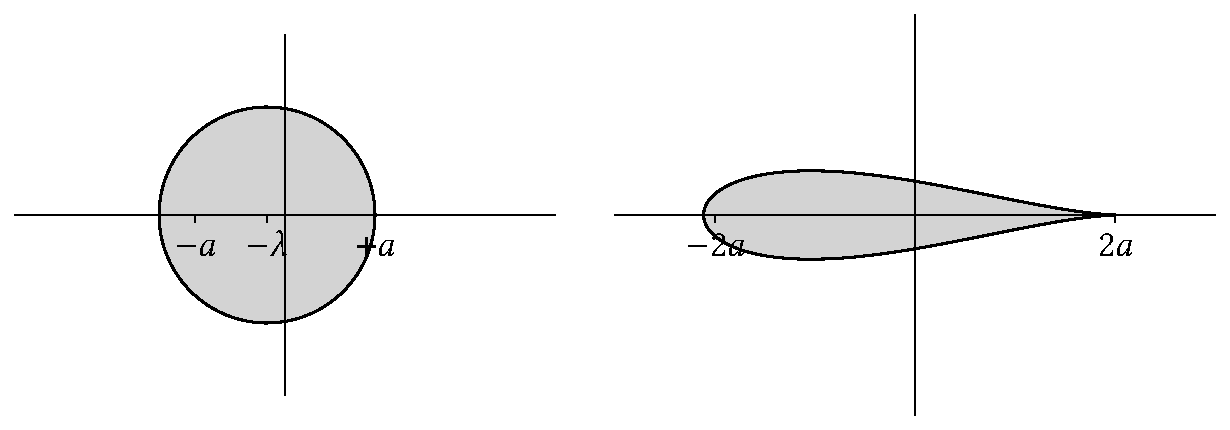
\includegraphics[width=\linewidth]{Figures/Chapter4/fig_aerofoil}
\caption{The Joulowski transformation takes the circle, shifted to the left by an amount $\lambda$, into an aerofoil shape.}
\label{fig_aerofoil}
\end{figure}

The complex potential around the shifted circle can be found by replacing $z$ with $z+\lambda$ and $a$ with $a+\lambda$, and it becomes
\begin{equation}
w(z) = U\left[ (z+\lambda) e^{-i\alpha} + \frac{(a+\lambda)^2}{z+\lambda} e^{i\alpha} \right] - \frac{i\Gamma}{2\pi} \ln (z+\lambda).
\end{equation}
As usual, to find the complex potential $W(Z)$ around the aerofoil, we replace $z$ with $Z$ using the inverse Joukowski transform, equation (\ref{eq_inverse_jt}).  Feel free to try that on your own.  But we can also examine the velocity of the flow around the aerofoil with the same trick we did above -- using equation (\ref{eq_UV}):
\begin{equation}
\U - i\V = \frac{dw/dz}{f'(z)} = \frac{ U e^{-i\alpha} - Ue^{i\alpha} (a+\lambda)^2 / (z+\lambda)^2 - i\Gamma / 2\pi(z+\lambda)}{1-a^2/z^2}
\end{equation}
From this equation, it looks like we still have singularities at $z=\pm a$ or $Z = \pm 2a$.  However, if we once again specify the circulation, we can remove the singularity at $z=+a$; we need to set 
\begin{equation}
\Gamma = -4\pi U (a + \lambda) \sin \alpha
\end{equation}
for the flow to remain finite there.  If the aerofoil is ``thin,'' so that $\lambda \ll a$, then $\Gamma$ reduces to that for the flat plate.  This value of the circulation is called the \emph{Kutta-Joukowski condition}, something we'll discuss in more depth momentarily.

What about the singularity at $z = -a$ or $Z = -2a$?  We don't have to worry about that one -- it's covered by the aerofoil, and so there is no fluid there.  Our trick worked, and as long as we have the right circulation, the flow is everywhere finite around the wing.  The streamlines are shown in Figure \ref{fig_aerofoil_stream}.

\begin{figure}
\centering\includegraphics[width=\linewidth]{Figures/Chapter4/fig_aerofoil_stream}
\caption{The streamline and pressure of the flow around an aerofoil.  Here $\alpha = \pi/6$, $\Gamma = -4\pi U(a+\lambda) \sin \alpha$, and $\lambda = 0.2$.}
\label{fig_aerofoil_stream}
\end{figure}

Now that we have the velocity $[\U, \V]$ of the fluid around the aerofoil, we could in principle find the pressure from Bernoulli's principle -- we're still dealing with steady, irrotational flow, so $H$ is constant within the fluid, and we can write
\[
\frac{p_\infty}{\rho} + \frac{1}{2} U^2 = \frac{p(s, \phi)}{\rho} + \frac{1}{2} \vec{u}^2,
\]
calculate $\vec{u}^2 = \U^2 + \V^2$ and solve for the pressure $p(s, \phi)$.  As usual, that's a complicated procedure by hand, but easier with a computer, and Figure \ref{fig_aerofoil_stream} shows the pressure around the aerofoil.

Then, given the pressure, we could integrate around the aerofoil to find the force -- again, too complicated for us to do here.  But it \emph{is} possible to do using more advanced complex analysis techniques, and it turns out that, regardless of the shape of the object, the result is always the same:
\begin{equation}
\vec{F} = - \rho U \Gamma \, \unit{y},
\end{equation}
where the coordinate system is chosen such that the uniform flow far away is directed along the positive $x$ axis.  This is the same result as for a circular cylinder, equation (\ref{eq_force1}), and it's correct for the aerofoil as well.  This general result is called the \emph{Kutta-Joukowski theorem.}

That brings us finally to a classic fluid dynamics question:  how do airplanes fly?  The answer, of course, as anyone who has stuck their hand out the window of a moving car knows, is that the wing deflects the air downward, causing an upward force on the wing itself.  However, the Kutta-Joukowski condition and theorem give an alternative explanation.

We need two bits of information.  First, recall Kelvin's Circulation Theorem from Section \ref{sec_circulation}, which says that the circulation $\Gamma$ around a dyed, closed curve $C(t)$ in the fluid is constant.  And second, we know that for there to be a singularity-free flow around an aerofoil, there must be circulation $\Gamma = -4\pi Ua \sin \alpha$, and that this circulation is what provides upward lift on the aerofoil.  Consider, then, what happens as an airplane starts moving down the runway to take off -- see Figure \ref{fig_airplane}.

When the airplane is initially at rest, before starting takeoff (top panel), the circulation around the curve $C(t)$ is obviously \emph{zero} -- the wing and fluid are at rest.  Then the wing starts to move to the left, or, as in our reference frames above where the object is at rest, the fluid starts to move to the right.  For there to be no singularities in the flow, there must be circulation around the wing -- but the \emph{total} circulation is still zero from Kelvin's Circulation Theorem.  So there must be some \emph{additional} circulation within $C(t)$, and in the opposite sense to balance out.  This is called a \emph{starting vortex}, and is easily seen in real airplanes or even with some water, food colouring, and a plastic card, as shown in Figure \ref{fig_starting_vortex}.  Notice the vortex is counterclockwise, as expected.  Why does the airplane fly?  Because the circulation generated around the wing provides \emph{lift}.  As the airplane travels faster (so larger $U$), both the circulation and the lift force increase.

\begin{figure}
\centering\includegraphics[width=0.8\linewidth]{Figures/Chapter4/fig_airplane}
\caption{An airplane taking off induces a starting vortex.}
\label{fig_airplane}
\end{figure}

\begin{figure}
\centering\includegraphics[width=0.8\linewidth]{Figures/Chapter4/fig_starting_vortex}
\caption{Put some water in a shallow container, place a small plastic card in the fluid, and put a small drop of food colouring at the edge of the card.  Drag the card to the left, keeping the angle of attack consistent, and the dye will trace out the starting vortex.}
\label{fig_starting_vortex}
\end{figure}

%
%  SECTION 4.3 - VORTEX MOTION
%

\section{Vortex Motion}

% SECTION 4.3.1 - THE HELMHOLTZ VORTEX THEOREMS

\subsection{The Helmholtz Vortex Theorems}

We've investigated flows involving vorticity throughout the book, and the time has come to properly define a \emph{vortex line} -- not quite the same thing as a line vortex flow -- and a \emph{vortex tube}.  

A vortex line is a curve in the fluid which, at some time $t$, has the same direction as the vorticity,
\[
\vec{\omega} = \grad \times \vec{u}
\]
at each point (see left panel of Figure \ref{fig_vortex_tube}).  Essentially that makes vortex lines similar to stream lines, but for vorticity $\vec{\omega}$ rather than the velocity $\vec{u}$.  A vortex tube is a bundle of vortex lines -- it's formed, again at some time $t$, by all vortex lines passing through a closed curve $C_1$ (see the right panel of Figure \ref{fig_vortex_tube}).  

\begin{figure}
\centering\includegraphics[width=0.8\linewidth]{Figures/Chapter4/fig_vortex_tube}
\caption{Left: The tangent of each point on a vortex line has the same direction as the vorticity $\vec{\omega}$.  Right: A vortex tube is the collection of vortex lines that lie along a closed curve in the fluid.}
\label{fig_vortex_tube}
\end{figure}

For an ideal fluid, Helmholtz formulated a number of theorems\footnote{I've seen textbooks list two, three, or four theorems; I'll state three here, but the essential ideas are all the same.} about the appearance and motion of vortex lines and tubes:

\begin{theorem}[Helmoholtz's Vortex Theorems]
\begin{enumerate}
\item Vortex lines move with the fluid.
\item The strength of a vortex tube is constant.
\item A vortex tube cannot end within the fluid -- it must end on a solid boundary, a free surface, or form a closed loop.
\end{enumerate}
\end{theorem}

Of these, the first is most important to our purpose here, and I'll sketch a brief proof.  Consider the surface $S$ on the vortex tube as shown in Figure \ref{fig_vortex_tube} -- $S$ is on the surface of the vortex tube itself, so that its area vector $\unit{n}$ is perpendicular to the vorticity $\vec{\omega}$ of each vortex line.  If that's the case, then the circulation around the perimeter of $S$ must be zero. We can see this from equation (\ref{eq_circ_curl}), which says the circulation can be calculated from
\[
\Gamma = \int_S \vec{\omega} \cdot d\vec{a}.
\]
Since the area vector is always perpendicular to the vorticity, the dot product is zero and $\Gamma = 0$ around this surface.  Kelvin's circulation theorem ensures that $\Gamma = 0$ always for the surface $S$, so that even as the fluid moves, $S$ remains on the surface of the vortex tube; since $S$ is an arbitrary surface and could be anywhere, the conclusion is that as the fluid moves, the vortex tube remains a vortex tube and moves with the fluid.  Taking the vortex tube to be infinitesimally thin gives us a vortex line, proving Helmholtz's first theorem.

% SECTION 4.3.2 - A VORTEX PAIR

\subsection{A Vortex Pair}

The practical result of this theorem can be seen by considering two vortexes, separated by a distance $2d$ and having opposite circulation but equal strength; this is the same flow we've seen before for a vortex beside a wall (Section \ref{sec_images}), but here we'll actually consider both vortexes in the fluid.  Helmholtz's first theorem says that each vortex will move with the fluid -- in this case, the vortex on the left will have an effect on the one on the right, and vice versa.  To see what effect they have on each other, take a look at Figure \ref{fig_vortex_pair1} and consider first the left vortex.  The fluid velocity due to it is given by
\[
\vec{u} = \frac{\Gamma}{2\pi s} \, \unit{\phi},
\]
which at the position of the right vortex is
\[
\vec{u} = -\frac{\Gamma}{4\pi d} \, \unit{y}.
\]
Evidently, the left vortex causes the right vortex to move \emph{down} along the negative $y$ direction.  Note that the right vortex has no effect on itself -- it can't push on itself any more than a charged particle can create an electric force on itself. 

\begin{figure}
\centering\includegraphics[width=0.8\linewidth]{Figures/Chapter4/fig_vortex_pair1}
\caption{Two vortexes of equal but opposite circulation, a distance $2d$ apart.  The left vortex induces a fluid velocity $\vec{u}_\text{L}$ at the position of the right vortex, and the right vortex induces a velocity $\vec{u}_\text{R}$ at the left.}
\label{fig_vortex_pair1}
\end{figure}

If we look at the effect of the right vortex on the left, we get a similar result:  the right causes the left to move downward with the same speed.  Both vortexes move together, in lockstep, with speed
\begin{equation}
V = \frac{\Gamma}{4\pi d}.
\end{equation}
It's actually quite easy to create a vortex pair like this; dragging a small plate through water will do it, with a vortex formed at each edge of the plate.  Once the plate is removed, the vortexes will continue to move due to each other's influence.  Figure \ref{fig_vortex_pair_pool} shows a vortex pair moving across a small pool.

\begin{figure}
\centering\includegraphics[width=0.9\linewidth]{Figures/Chapter4/fig_vortex_pair_pool}
\caption{It's possible to create a vortex pair by dragging a small plate through a pool of water.  The starting vortexes that form are equal in strength and opposite in direction, and they travel across the pool at constant speed and without losing strength.}
\label{fig_vortex_pair_pool}
\end{figure}

If we want to model the vortex pair, we can shift to a reference frame in which they are at rest so that the overall flow is steady.  That means we'll need to include, in addition to the two vortexes, a uniform flow with speed $V$ moving upward.  The complex potential of uniform flow is
\[
w_\text{uni}(z) = Uze^{-i\alpha},
\]
and to have the flow move upward along $+\unit{y}$, we'll set $\alpha = \pi/2$, so that $e^{-i\pi/2} = -i$.  With $U = V = \Gamma/4\pi d$ we have
\[
w_\text{uni}(z) = -\frac{i\Gamma z}{4\pi d}.
\]
The full complex potential, including the two opposite but equal vortexes, would be
\begin{equation}
w(z) = -\frac{i\Gamma z}{4\pi d} - \frac{i\Gamma}{2\pi} \ln (z-d) + \frac{i\Gamma}{2\pi} \ln (z+d),
\end{equation}
and streamlines for this flow are shown in Figure \ref{fig_vortex_pair3}.

\begin{figure}
\centering\includegraphics[width=0.7\linewidth]{Figures/Chapter4/fig_vortex_pair3}
\caption{Streamlines for the flow in a reference frame in which the vortex pair is at rest.}
\label{fig_vortex_pair3}
\end{figure}

Are the vortexes actually at rest in this reference frame?  We can check easily enough by calculating their speed.  Let's start with the derivative of the complex potential,
\begin{equation}
\label{eq_vortex_pair}
\frac{dw}{dz} = u - iv = -\frac{i\Gamma}{4 \pi d} - \frac{i\Gamma}{2\pi} \frac{1}{z-d} +  \frac{i\Gamma}{2\pi} \frac{1}{z+d}.
\end{equation}
To find the speed of the vortex on the right, we evaluate this derivative at its location, $z = d$:
\[
u_R - iv_R = \left. \frac{dw}{dz} \right|_{z=d}.
\]
But be careful here: the right vortex won't be affected by itself, so we'll ignore that particular term --the second -- in equation (\ref{eq_vortex_pair}).  The speed of the right vortex becomes
\[
u_R - iv_R = -\frac{i\Gamma}{4\pi d} + \frac{i\Gamma}{2\pi} \left( \frac{1}{2d} \right) = 0.
\]
So, as expected, $u_R = 0$ and $v_R = 0$ -- the vortex on the right is at rest in this reference frame.  Similarly for the vortex on the left.


% SECTION 4.3.3 - VORTEX SHEDDING

\subsection{Vortex Shedding}

We've been discussing ideal fluids exclusively for the last two chapters, and will continue with them for the next one as well.  But I want to return for a moment to the major difference between viscous and inviscid flow at high Reynolds number: the presence of a boundary layer.  In an ideal fluid, flow around a circular cylinder looks like our solution (Figures \ref{fig_uniform_circle} and \ref{fig_cylinder_circ}) regardless of how fast the fluid is flowing.  In reality, for high speed flow (or equivalently high Reynolds number flow), the viscous boundary layer plays an important role in the behaviour of the fluid downstream.  

\begin{figure}
\centering\includegraphics[width=0.9\linewidth]{Figures/Chapter4/fig_vortex_shedding}
\caption{Computational fluid dynamics simulation past a circular cylinder.  The popular open source code SU2 was used.  (a) Reynolds number $R = 10$.  A vortex pair is formed on the trailing side shortly after the flow is started.  (b) $R = 30$.  The region in which the fluid reverses is larger.  (c) and (d) $R = 10,000$.  The flow becomes unsteady and asymmetric (c), and eventually (d) the vortexes begin to detach and are shed downstream.}
\label{fig_vortex_shedding}
\end{figure}

To illustrate this, Figure \ref{fig_vortex_shedding} shows a computational fluid dynamics simulation of viscous flow past a circular cylinder.  At low Reynolds number (between five to 40 or so), the boundary layer at the trailing edge of the surface grows; this boundary layer is high in vorticity and eventually two small vortexes appear.  These vortexes are equal in strength and opposite in direction -- the flow \emph{reverses} near the trailing stagnation point.  Figure \ref{fig_vortex_shedding}$a$ shows the vortexes for $R = 10$; at slightly higher Reynolds number ($R = 30$) these vortexes are larger as in Figure \ref{fig_vortex_shedding}$b$.  However, at Reynolds number greater than around 40, something interesting happens:  the vortexes become \emph{unstable} and one grows in size over the other (Figure \ref{fig_vortex_shedding}$c$).  The larger vortex then detaches from the cylinder and travels downstream (Figure \ref{fig_vortex_shedding}$d$), forming a wake.  This process is called \emph{vortex shedding}, and the wake has a highly structured form, something we'll consider in depth in a moment.  

Before we consider the wake, however, I'd like to try modelling the initial phase of vortex shedding -- the steady vortexes that are attached to the trailing edge of the cylinder.  We can approximate these attached vortexes as ideal line vortexes, but it turns out that adding them to a circular cylinder is a little difficult.  Instead, we can simplify the situation a by using a flat boundary at $x = 0$, as shown in Figure \ref{fig_attached_vortex1}.  Now, that's definitely not a curved circular surface, but as long as we imagine the circle is large and the vortexes close to it, it doesn't do too bad a job.

\begin{figure}
\centering\includegraphics[width=0.75\linewidth]{Figures/Chapter4/fig_attached_vortex1}
\caption{Modelling the attached vortexes requires mirror images for each.  Note the circulation directions and positions of each vortex.}
\label{fig_attached_vortex1}
\end{figure}

We can model the flow around the ``circle'' with the stagnation point flow, 
\[
w(z) = \frac{1}{2} \alpha z^2,
\]
as shown in the light grey lines in Figure \ref{fig_attached_vortex1}.  The vortexes will be added to this flow, but we have to be careful.  There's a boundary at $x=0$ and we must ensure the flow meets the boundary conditions there -- that is, it has to slip along that wall.  But we already know how to handle this -- with method of images.  So in addition to the two vortexes we want in our flow, we also need two mirror vortexes on the other side of the wall with opposite circulation; that will give us the correct boundary, as you can check for yourself.  So, we need four vortexes, all the same strength, but with two having counterclockwise circulation (positive $\Gamma$) and two having clockwise (negative $\Gamma$).  Setting the position $z_0$ of the top right vortex fixes all the others in place.  If
\[
z_0 = d + id,
\]
then the lower right vortex is at $d - id = z_0^*$, the upper left is at $-d + id = -z_0^*$, and the lower left vortex is at $-d -id = -z_0$.  The full complex potential, including the background stagnation point flow, will be
\begin{equation}
\label{eq_w_vortex_shedding}
w(z) = \frac{1}{2} \alpha z^2 + \frac{i\Gamma}{2\pi} \ln (z - z_0) -  \frac{i\Gamma}{2\pi} \ln (z - z_0^*) -  \frac{i\Gamma}{2\pi} \ln (z + z_0^*) +  \frac{i\Gamma}{2\pi} \ln (z + z_0).
\end{equation}

Only for one particular choice of $d$, however, will the vortexes be at rest -- and so ``attached'' to the cylinder.  Problem \ref{prob_attached_vortexes} asks you to find this; the answer is
\begin{equation}
d = \sqrt{\frac{\Gamma}{8 \pi \alpha}}.
\end{equation}
Once we have the correct complex potential, we can find the streamlines from $\phi = \operatorname{Im}(w)$ as usual, and, if we want, the pressure from Bernoulli's theorem.  Figure \ref{fig_attached_vortex2} shows the vortexes and pressure; it's up to you to compare with Figure \ref{fig_vortex_shedding} and see if our model does a reasonable job at reproducing it.  Note, however, that although the vortexes are \emph{steady} when placed at $d \pm id$, they're also \emph{unstable} and would detach with any kind of perturbation.

\begin{figure}
\centering\includegraphics[width=0.5\linewidth]{Figures/Chapter4/fig_attached_vortex2}
\caption{Streamlines and pressure field for the attached vortexes.}
\label{fig_attached_vortex2}
\end{figure}


% SECTION 4.3.4 - VON KARMAN VORTEX STREET

\subsection{The von K\'arm\'an Vortex Street}

Under the right conditions, the wake created by vortex shedding from a cylinder or other object can be highly structured and periodic -- the vortexes form a \emph{von K\'arm\'an vortex street,}  in which vortexes travel downstream from the object in two separate lines.  This is frequently seen in nature when wind blows past an island mountain in the ocean and surrounding clouds form the vortex street; examples are shown in Figure \ref{fig_vortex_street_clouds}.  It's also readily seen in fluid simulations such as the one in Figure \ref{fig_vortex_shedding}, and, since it is at least approximately steady state, it's amenable to a simple model.

\begin{figure}
\centering\includegraphics[width=0.9\linewidth]{Figures/Chapter4/fig_vortex_street_clouds}
\caption{Examples of vortex streets forming in clouds as the air moves past islands in the ocean.  All photos from NASA.}
\label{fig_vortex_street_clouds}
\end{figure}

As we did above, we'll model each vortex in the street as a line vortex, but since we're approximating this as a steady state, we'll need an infinite number of them in two rows.  Imagine that an object exists far to the left, and uniform flow to the right past this object creates a vortex street.  We'll stagger the vortexes as shown in Figure \ref{fig_vortex_street1}.  Note the orientation of each vortex -- along the top row, they have clockwise (negative $\Gamma$) circulation, while each vortex in the bottom row circulates in a counterclockwise (positive $\Gamma$) fashion.  Each vortex is separated by their neighbours in their line by a distance $a$, the the two lines are separated by a distance $b$.


\begin{figure}
\centering\includegraphics[width=0.7\linewidth]{Figures/Chapter4/fig_vortex_street1}
\caption{Model of a vortex street:  two infinite lines of vortexes, with each line having opposite rotation.}
\label{fig_vortex_street1}
\end{figure}


Our objective will be to find the complex potential that describes the flow, but first we need to think about how this vortex street \emph{moves}.  Consider just one vortex -- the red one in Figure \ref{fig_vortex_street1}, which is located in the complex plane at 
\[
z = \frac{1}{2} a + ib.
\]
Remember, each of the vortexes in the street will move due to the influence of all the rest.  But for this vortex, the others  in the top row will have no effect -- because they're evenly spaced, they cancel in pairs, and the net result is that the fluid is at rest at the location of the red vortex.  The bottom row, however, does have an effect.  With a little bit of thought, you should be able to see that the fluid velocity at the position of the red vortex due to the bottom row is to the \emph{left}.

That the flow is to the left might sound strange at first -- we set up this problem so that the object creating the vortex street is far to the left and the flow is moving to the right.  But right now we're in the reference frame of the uniform flow itself -- we're moving to the right with it, and the vortexes in the street evidently move to the left in this frame.  That means that in the reference frame where the object is at rest, the vortexes will move to the \emph{right}, but more slowly than the uniform flow past the object.  We'll stick with the uniform flow reference frame for now, but can always add in a uniform flow later if we want to.

What exactly is the speed the vortexes move with?  To answer, we'll have to write down the complex potential for the bottom row -- I'll ignore the top row for now since it has no effect on the red vortex we're examining.  In principle the complex potential is simple to write down, although there are an infinite number of vortexes:
\[
w(z) = \cdots - \frac{i\Gamma}{2\pi} \ln (z + a) - \frac{i\Gamma}{2\pi} \ln (z) - \frac{i\Gamma}{2\pi} \ln (z - a) - \cdots
\]
Now, the $n$th term is
\[
w_n(z) = -\frac{i\Gamma}{2\pi} \ln (z - na),
\]
and $n$ will run from $-\infty$ to $\infty$.  But we can write this instead as
\[
w_n(z) = -\frac{i\Gamma}{2\pi} \ln \left(1 - \frac{z}{na} \right);
\]
it differs from the above only by a constant, which isn't important for the complex potential.  Then the full complex potential due to the bottom row is
\begin{equation}
w(z) = -\frac{i\Gamma}{2\pi} \sum_{n=-\infty}^{-1} \ln \left(1 - \frac{z}{na} \right) - \frac{i\Gamma}{2\pi} \ln z -\frac{i\Gamma}{2\pi} \sum_{n=1}^{\infty} \ln \left(1 - \frac{z}{na} \right).
\end{equation}
The first term handles all the vortexes to the left of the origin, the middle term the vortex at the origin itself, and the right term the vortexes to the right.  

This is correct, but we can simplify it quite a bit by doing some rearranging.  I'll write out some of the terms so we can see the pattern we're looking for better:
\begin{multline*}
w(z) = -\frac{i\Gamma}{2\pi} \biggl[ \ln z + \cdots + \ln \left(1 - \frac{z}{(-2a)} \right) +  \ln \left(1 - \frac{z}{(-a)} \right) + \\ \ln \left(1 - \frac{z}{a} \right) +  \ln \left(1 - \frac{z}{2a} \right) + \cdots \biggr]
\end{multline*}
We can use log rules to turn those additions of logs to multiplications within, getting
\[
w(z) = -\frac{i\Gamma}{2\pi} \ln \biggl[ (z) \cdots \left(1 - \frac{z}{(-2a)} \right) \left(1 - \frac{z}{(-a)} \right) \left(1 - \frac{z}{(a)} \right) \left(1 - \frac{z}{(2a)} \right) \cdots \biggr]
\]
At this point we can do some of the multiplication.  Consider the inner two terms - if we multiply them together we get a difference of squares,
\[
\left(1 - \frac{z}{(-a)} \right) \left(1 - \frac{z}{(a)} \right) = \left( 1 - \frac{z^2}{a^2} \right),
\]
and similarly with the outer two terms.  In fact, along the entire infinite number of terms, we can combine them in pairs so that we get
\[
w(z) = -\frac{i\Gamma}{2\pi} \ln \biggl[ z \prod_{n=1}^\infty \left( 1- \frac{z^2}{n^2 a^2} \right) \biggr].
\]
It turns out the thing in the square brackets is actually an infinite product expansion of the sine function, and we finally have 
\begin{equation}
\label{eq_vortex_street}
w(z) = -\frac{i\Gamma}{2\pi}\ln \biggl[ \sin \left( \frac{\pi z}{a} \right) \biggr].
\end{equation}

\begin{figure}
\centering\includegraphics[width=0.95\linewidth]{Figures/Chapter4/fig_vortex_street2}
\caption{Streamlines and pressure of the simple model for the vortex street.  Here $a = 1$ and $b = 0.2$ and the uniform flow velocity is $U = u_0$ so that the vortexes are at rest in this frame. }
\label{fig_vortex_street2}
\end{figure}

Now we can easily get the speed of the red vortex in Figure \ref{fig_vortex_street1}.  Taking the derivative gives
\[
u - iv = \frac{dw}{dz} = -\frac{i\Gamma}{2\pi} \cot \left( \frac{\pi z}{a} \right).
\]
This is the velocity of the fluid everywhere due to the bottom row only.  If we evaluate this at the location of the red vortex, $z = \tfrac{1}{2} a + ib$, we find
\[
u_0 - iv_0 = \left. \frac{dw}{dz} \right|_{z = \tfrac{1}{2} a + ib} = -\frac{\Gamma}{2a} \tanh \left( \frac{\pi b }{a} \right).
\]
That means the velocity components of the vortex are
\begin{equation}
\label{eq_vortex_street_speed}
u_0 = -\frac{\Gamma}{2a} \tanh \left( \frac{\pi b }{a} \right) \quad \text{and} \quad v_0 = 0.
\end{equation}
As expected, it moves to the left ($u_0$ is negative) and has no motion along the $y$ direction (see Problem \ref{prob_vortex_street}).

Now that we've analyzed the bottom row, we can easily repeat for the top to find the total complex potential.  The full complex potential everywhere is
\begin{equation}
w(z) = -\frac{i\Gamma}{2\pi}\ln \biggl[ \sin \left( \frac{\pi z}{a} \right) \biggr] + \frac{i\Gamma}{2\pi}\ln \biggl[ \sin \left( \frac{\pi (z - a/2 - ib)}{a} \right) \biggr] + Uz,
\end{equation}
where the last term allows for a uniform flow if we want to move to a reference frame in which it has a non-zero velocity.  Figure \ref{fig_vortex_street2} shows the streamlines and pressure for this complex potential, and I set $U = -u_0$, the speed at which the vortexes travel, so that they are at rest in the figure.  Again, it's up to you to decide how good the model is; compare with the cloud photographs or simulation images.




\section*{Problems}
\addcontentsline{toc}{section}{Problems}
\markright{Problems}%

\begin{problem}[Complex numbers]

(a) Show that $|z|^2$ is real using polar coordinates.

(b) Show that $1/i = -i$.

(c) Show that
\[
\sqrt{i} = \frac{1}{\sqrt{2}} + \frac{i}{\sqrt{2}}.
\]
\end{problem}


\begin{problem}[A line source]
\label{prob_line_source_w}
Starting from the velocity potential $\varphi(s, \phi)$ and stream function $\psi(s, \phi)$ , derive the complex potential for a line source of strength $Q$.
\end{problem}


\begin{problem}[Power law complex potentials]
Consider a general complex potential of the form $w(z) = Az^n$.  For $n = 2/3, 3/2, 2,$ and $n = 3$, plot the streamlines and physically interpret the flow.  Is there a relationship between the exponent $n$ and how the flow behaves?
\end{problem}

\begin{problem}[The doublet flow]
Of special interest is the power law flow with $n = -1$: $w(z) = A/z$.  For this flow, find the velocity potential and stream function as well as the velocity (use polar coordinates).  Plot the streamlines.
\end{problem}

\begin{problem}[Combination of flows]
Plot the streamlines for a flow that consists of a stagnation point of strength $\alpha = 1$ and a line vortex of strength $\Gamma = 10$ and positioned at $z = 1$.
\end{problem}

\begin{problem}[Boundary conditions from the mirror image]
\label{prob_mirror_bc}
Starting from equation (\ref{eq_mirror_vortex}), find the velocity of the fluid $[u, v]$ and show that the flow slips along the wall (in other words, shown that $u(0, y) = 0$).  Warning:  this will take a fair bit of algebra.
\end{problem}

\begin{problem}[A vortex in a corner]
Consider a vortex located at $z = a + ib$, where $a$ and $b$ are both positive, and there are boundaries as shown in Figure \ref{fig_vortex_corner}.  

(a) What is the complex potential for the fluid in the region $x \ge 0, y \ge 0$?

(b) Plot the streamlines for the region $x \ge 0, y \ge 0$.

(c) Show explicitly that the fluid velocity is zero at the corner.

(d) This vortex will \emph{move} due to the rest of the flow.  Show that the path the vortex takes is given by
\[
\frac{1}{x} + \frac{1}{y} = \text{constant}.
\]
\end{problem}

\begin{figure}
\centering\includegraphics[width=0.75\linewidth]{Figures/Chapter4/fig_vortex_corner}
\caption{A line vortex in a corner.}
\label{fig_vortex_corner}
\end{figure}

\begin{problem}[A line source by a wall]
Consider a line source $Q$ a distance $b$ from a boundary along $x = 0$ (so the fluid exists only in $x>0$).  Use the method of images to determine the complex potential, making sure to show explicitly that the boundary condition is satisfied (a drawing will do).  Then find the velocity $u$ of the flow and plot the streamlines.
\end{problem}

\begin{problem}[A line source by two walls]
Suppose there are two boundaries, one at $y = +b$ and one at $y = -b$, with fluid in between.  A line source $Q$ sits right in the middle at $y = 0$.  Show that the complex potential is
\[
w(z) = \frac{Q}{2\pi} \ln \left[ \sinh \left( \pi z / 2b \right) \right].
\]
\end{problem}

\begin{problem}[Using the circle theorem]
Consider the complex potential
\[
w(z) = \frac{A}{2} (z^2 - 2cz)
\]
where $A$ and $c$ are constants.  

(a) Find the velocity potential and the stream function and plot the streamlines.

(b) Add a circular cylinder to the flow using the Milne-Thomson circle theorem and find the new complex potential.  Show that the stream function is given by
\[
\psi(x, y) = Ay \left[ x \left( 1 + \frac{a^2}{x^2 + y^2} \right) - c\right] \left(1 - \frac{a^2}{x^2 + y^2} \right)
\]
and plot the new streamlines.
\end{problem}

\begin{problem}[Flow around a circular cylinder]
\label{prob_circlular_cylinder}
Equation (\ref{eq_uniform_circle}) gives the complex potential for flow around a circular cylinder, including an angle and circulation, but for this problem set $\alpha = 0$.  

(a) By taking the derivative of $w(z)$, show that the velocity is given by
\[
u_s(s, \phi) = U \left( 1 - \frac{a^2}{s^2} \right) \cos \phi \quad \text{and} \quad u_\phi(s, \phi) = -U \left( 1 + \frac{a^2}{s^2} \right) \sin \phi + \frac{\Gamma}{2\pi s}.
\]

(b) Show that there are two stagnation points on the cylinder (at $s = a$) if the circulation is $\Gamma < 4\pi U a$, only one point if $\Gamma = 4\pi U a$, and none if $\Gamma > 4\pi U a$. 

(c) Where is the stagnation point in the fluid if $\Gamma = 8 \pi U a$?  (Hint: it's not on the boundary $s=a$.)
\end{problem}

\begin{problem}[Force on a circular cylinder]
\label{prob_force2}
Problem \ref{prob_force1} asked you to calculate the force on a cylinder from an ideal fluid.  Repeat that calculation, but this time include \emph{circulation} $\Gamma$ (you can set $\alpha = 0$, though), and show that
\[
F_x = 0 \quad \text{and} \quad F_y = -\rho U \Gamma.
\]
\end{problem}

\begin{problem}[Flow around an ellipse and a flat plate]
\label{prob_flat_plate}

(a) Starting from the complex potential for flow past a circular cylinder (equation \ref{eq_uniform_circle}), use the inverse Joukowski transform to derive the flow past an elliptical cylinder (equation \ref{eq_ellipse_w}).

(b) With $c = a$ in the Joulowski transform, the ellipse becomes a flat plate.  Using equation (\ref{eq_dwdz}), show that the singularity in the flow at $z = +a$ disappears if the circulation is $\Gamma = -4\pi U a \sin \alpha$, and show that the flow at that point is
\[
\U = U \cos \alpha \quad \text{and} \quad \V = 0.
\]
\end{problem}

\begin{problem}[Attached Vortexes]
\label{prob_attached_vortexes}
Equation \ref{eq_w_vortex_shedding} gives the complex potential for a pair of attached vortexes.  By taking the derivative of this expression and evaluating it at the location of each vortex, show that the vortexes are at rest if
\[
d = \sqrt{\frac{\Gamma}{8\pi \alpha}}.
\]
\end{problem}

 
\begin{problem}[The vortex sptreet]
\label{prob_vortex_street}
For the vortex street, the complex potential for the bottom row is given by equation (\ref{eq_vortex_street}).  From this, show that the velocity of the red vortex in Figure \ref{fig_vortex_street1} is given by equation (\ref{eq_vortex_street_speed}).
\end{problem}



\chapter{Waves}

%
%  SECTION 5.1 - XXX
%





\chapter{Special Topics}

%
%  SECTION 6.1 - Navier-Stokes
%

\section{Deriving the Navier-Stokes Equation}
\label{sec_ns_deriv}

As we'll see, the Navier-Stokes equation follows directly from Newton's second law; however, because it depends on the \emph{deformation} of fluid elements, we need a whole new framework to describe the forces at work. 

\subsection{The Stress Tensor and Vector}

To start, let's consider a fluid element -- I'll draw it as a cube for simplicity but it can be any shape (Figure \ref{fig_deform}).  If we apply a force that's normal to a surface, we'd expect the fluid element to deform by stretching and thinning.  On the other hand, if the \emph{same} force, in the same direction, is applied to a surface that's parallel to it, the deformation will be very different -- the force in this case is called a ``shear force.''  Evidently, the deformation of a fluid element depends not only on the force direction but also on the \emph{surface} direction. 

\begin{figure}
\centering
\includegraphics[width=0.9\linewidth]{Figures/Chapter2/fig_deform}
\caption{The deformation of a fluid element depends on both the force direction \emph{and} the direction of the surface. }
\label{fig_deform}
\end{figure}

This, unfortunately, adds a complication to how we must describe the forces that deform a fluid element.  There are three orthogonal directions that the force itself could have, and three orthogonal directions that surface it's applied to could have -- that means we need nine different numbers to fully specify things.  Figure \ref{fig_stress_tensor} shows this graphically; the nine elements together are called the \emph{stress tensor} and are labelled $T_{ij}$, where $i$ specifies the direction of the force, and $j$ the direction of the surface.  The elements of the stress tensor are forces per unit area; for example, the element $T_{xy}$ gives the stress, or force per unit area, acting in the $\unit{x}$ direction on a surface with normal in the $\unit{y}$ direciton.

\begin{figure}
\centering
\includegraphics[width=0.7\linewidth]{Figures/Chapter2/fig_stress_tensor}
\caption{The definition of the stress tensor.}
\label{fig_stress_tensor}
\end{figure}

It's common to write the tensors using either ``index notation,'' like $T_{ij}$, or as a matrix:
\[
\tens{T} = \begin{bmatrix}
T_{xx} & T_{xy} & T_{xz} \\
T_{yx} & T_{yy} & T_{yz} \\
T_{zx} & T_{zy} & T_{zz} 
\end{bmatrix}.
\]
Note that the notation for a tensor, $\tens{T}$, is a little different from vectors.  And it turns out that in almost all cases the stress tensor is \emph{symmetric}, so that 
\[
T_{ij} = T_{ji},
\]
which means that we really only have six elements to worry about rather than the full nine.

Suppose we have some surface $S$ with a normal vector $\unit{n}$; the \emph{stress vector} is defined as 
\begin{equation}
\vec{t} = \tens{T} \cdot \unit{n}.
\label{eq_stress}
\end{equation}
Careful here -- that's a dot product between a tensor and a vector, not two vectors, and the result is a vector rather than a scalar.  We can calculate the dot product either by direct summation,
\[
t_i = \sum_{j=1}^3 T_{ij} n_j.
\]
or by matrix multiplicaiton,
\[
\vec{t} = \begin{bmatrix}
T_{xx} & T_{xy} & T_{xz} \\
T_{yx} & T_{yy} & T_{yz} \\
T_{zx} & T_{zy} & T_{zz} 
\end{bmatrix}
\begin{bmatrix}
n_x  \\
n_y  \\
n_z  
\end{bmatrix}.
\]

As a check, let's suppose we have a surface where $\unit{n} = \unit{x}$.  In that case, the stress vector will be
\[
\vec{t} = \begin{bmatrix}
T_{xx} & T_{xy} & T_{xz} \\
T_{yx} & T_{yy} & T_{yz} \\
T_{zx} & T_{zy} & T_{zz} 
\end{bmatrix}
\begin{bmatrix}
1  \\
0  \\
0  
\end{bmatrix} = 
\begin{bmatrix}
T_{xx}  \\
T_{yx}  \\
T_{zx}  
\end{bmatrix},
\]
which makes sense -- the dot product picks out the forces that act on the surface with normal $\unit{x}$.

\subsection{Cauchy's Equation of Motion}

Now we're ready to use Newton's second law to derive a general equation of motion for fluids and other deformable materials.  Consider some ``blob'' of our fluid, with volume $V$ and enclosed by surface $S$; this blob can deform in shape as the fluid moves, but we'll assume our fluid is incompressible, so the total volume can't change.  The force across one small element of area, $dS$, due to the fluid above it, is given by the stress vector $\vec{t}$ multiplied by the area $dS$.  The total force acting on the entire blob due to the surrounding fluid is therefore
\begin{equation}
\vec{F} = \int_S \vec{t} \, dS = \int_S (\tens{T} \cdot \unit{n}) \, dS,
\end{equation}
where I used equation \ref{eq_stress} to write the force in terms of the stress tensor instead of the stress vector.  Now, we can apply the divergence theorem to turn this into an integral over the volume -- even though this is a tensor, it works pretty much the same way:
\[
\vec{F} =  \int_S (\tens{T} \cdot \unit{n}) \, dS = \int_V (\grad \cdot \tens{T} ) \, dV.
\]

So far, we've ignored any forces external to the fluid, but we can add them in now.  I'll stick with gravity; for a small volume of the fluid, the force of gravity will be $\rho dV \vec{g}$, and we can combine this with the stress force above to get
\[
\vec{F} = \int_V (\grad \cdot \tens{T} + \rho \vec{g} ) \, dV.
\]

That's the total force acting on our fluid, and we already know how to write out the acceleration -- that was equation \ref{eq_accel},
\[
\frac{D \vec{u}}{Dt} = \frac{\partial \vec{u}}{\partial t} + (\vec{u} \cdot \vec{\nabla}) \vec{u}.
\]
Newton's second law then gives
\[
\int_V \rho \frac{D \vec{u}}{Dt} \, dV = \int_V (\grad \cdot \tens{T} + \rho \vec{g} ) \, dV.
\]
But this equation holds for \emph{any} volume of any size within our fluid, so the integrands must be equal:
\begin{equation}
\boxed{
\rho \frac{D \vec{u}}{Dt} =\grad \cdot \tens{T} + \rho \vec{g}.
}
\label{eq_cauchy}
\end{equation}
This is called Cauchy's equation of motion.

\subsection{Newtonian Fluids}

So far we've been very general with the stress tensor; specifying different tensors gives us different fluids modelled with Cauchy's equation.  As a first example of a specific stress tensor -- the simplest possible one! -- consider 
\begin{equation}
T_{ij} = -p \, \delta_{ij},
\end{equation}
where $p(x, y, z, t)$ is a scalar function -- it's the \emph{pressure} in the fluid -- and $\delta_{ij}$ is called the Kronecker delta.  If you're not familiar with it, this is a handy function (technically, it's a tensor) that is \emph{one} if the two indices are the same, and \emph{zero} if there's different:
\[
\delta_{ij} = \begin{cases}
0 & i \neq j, \\
1 & i = j \end{cases}.
\]
As a matrix, this stress tensor therefore looks like
\begin{equation}
\tens{T} = \begin{bmatrix}
-p & 0 & 0 \\
0 & -p & 0 \\
0 & 0 & -p
\end{bmatrix}.
\label{eq_stress_ideal}
\end{equation}
This stress tensor defines \emph{ideal fluids}, which are inviscid (no viscosity) and don't include forces of deformation in the stress tensor.  Why the negative sign on the pressure?  Because this is the force of the fluid \emph{outside} the surface pushing on it -- in the opposite direction of the normal vector $\unit{n}$.

Although ideal fluids will make up a large part of our discussion of fluid dynamics, we're here to derive the Navier-Stokes equations, which deal instead with \emph{Newtonian fluids}, which do include the deformation of fluid elements.  To incorporate that, we'll add a term to the ideal fluid stress tensor:
\begin{equation}
T_{ij} = T_{ij}^I + T_{ij}^D,
\end{equation}
where the $I$ indicates the ideal part and the $D$ indicates the part that deals with the deformation.  

Consider, for a moment, a \emph{solid} instead of a fluid.  If the solid is elastic, then pushing on it will cause it to deform in shape, and the stress that results will be proportional to the change in shape.  This makes sense -- it's just like in Hooke's law, where the force of the spring is proportional to the displacement.  A fluid, though, is very different -- pushing on a fluid causes deformation, but the deformation continues even when the force is stopped.  It turns out that for fluids, the stress is proportional to the \emph{velocities} of the change in shape; that is, rather than
\[
t \propto dx,
\]
we have
\[
t \propto du/dx,
\]
for example.  Note a couple of things here:  first, there are three velocities, $u, v, w$, and three directions, $x, y, z$, so we have nine different velocity gradients we can form.  And second, note that these are derivatives with respect to \emph{position}, not time; these are not accelerations.

Now, the most general symmetric tensor that depends \emph{linearly} on these velocity gradients can be written as
\begin{equation}
T_{ij}^D = \mu \left( \frac{\partial u_j}{\partial x_i} + \frac{\partial u_i}{\partial x_j} \right),
\end{equation}
where $\mu$ is the constant of proportionality and is called (of course) the \emph{viscosity}.  Splitting the velocity gradients into two terms likes this ensures the tensor is symmetric.  Although it's cumbersome to do so, and doesn't really gain us anything, I'll write out this tensor in matrix form (you can at least compare with the ideal case in equation \ref{eq_stress_ideal}):
\[
\tens{T}^D = \begin{bmatrix}
2 \mu \partial u / \partial x  &  \mu (\partial v / \partial x + \partial u / \partial y)  &   \mu (\partial w / \partial x + \partial u / \partial z) \\
\mu (\partial u / \partial y + \partial v / \partial x)  & 2\mu  \partial v / \partial y  &  \mu (\partial w / \partial y + \partial v / \partial z) \\
\mu (\partial u / \partial z + \partial w / \partial x)  &  \mu (\partial v / \partial z + \partial w / \partial y) & 2\mu  \partial w / \partial z
\end{bmatrix}.
\label{eq_stress_newtonian}
\]

Adding in the ideal component, the total stress tensor is
\begin{equation}
\boxed{
T_{ij} = -p \delta_{ij} +  \mu \left( \frac{\partial u_j}{\partial x_i} + \frac{\partial u_i}{\partial x_j} \right).
}
\end{equation}
This defines a \emph{Newtonian fluid}.  But you should know that there's plenty of examples of \emph{non-Newtonian fluids,} as well -- paint and blood are two good examples.  Non-Newtonian fluids can be nonlinear in the velocity gradients, and can sometimes depend not just on the current state of the fluid, but on the past state as well -- some of these fluids can have a ``memory.''  These kinds of fluids are well outside the scope of this book, however.

\begin{example}[Plane parallel shear flow]
Recall our example from Section \ref{sec_imp} -- we had an impulsively moved boundary, which put the fluid into plane parallel shear flow given in general by $u(y)$.  For simplicity, we'll suppose the boundary is at $y=0$ and the flow exists above it.  What is the stress on the boundary from the fluid?

For flow of this type, the stress tensor becomes
\begin{equation}
\tens{T} = \begin{bmatrix}
-p & \mu \partial u / \partial y & 0 \\
\mu \partial y / \partial y & -p & 0 \\
0 & 0 & -p
\end{bmatrix},
\end{equation}
and we can calculate the stress vector using equation \ref{eq_stress}, with $\unit{n} = \unit{y}$ for the boundary surface:
\[
\vec{t} = \begin{bmatrix}
-p & \mu \partial u / \partial y & 0 \\
\mu \partial y / \partial y & -p & 0 \\
0 & 0 & -p
\end{bmatrix}
\begin{bmatrix}
0 \\ 1 \\ 0
\end{bmatrix}.
\]
Carrying out the matrix multiplication gives
\[
\vec{t} = \mu \frac{\partial u}{\partial y} \unit{x} - p \unit{y}.
\]
This result makes sense: there's a viscous force along the boundary caused by friction with the fluid, and a force pushing downward on the surface from the fluid above.
\end{example}

We're finally ready to derive the Navier-Stokes equation, which is just Cauchy's equation of motion with the stress tensor for Newtonian fluids.  I'm going to write out the calculation in index notation, which is a little easier to deal with, starting with Cauchy's equation,
\[
\rho \frac{Du_i}{Dt} = \sum_{j=1}^3 \frac{\partial T_{ij}}{\partial x_j} + \rho g_i
\]
(compare with the vector version in equation \ref{eq_cauchy}).  We only tricky thing here is the divergence of the stress tensor,
\[
\sum_{j=1}^3 \frac{\partial T_{ij}}{\partial x_j} = \sum_{j=1}^3 \frac{\partial }{\partial x_j} \left[ -p \delta_{ij} + \mu \left( \frac{\partial u_j}{\partial x_i} + \frac{\partial u_i}{\partial x_j} \right) \right],
\]
which is three derivatives.  We'll tackle each separately.

First is the pressure term,
\[
\sum_{j=1}^3 \frac{\partial }{\partial x_j} \left( -p \delta_{ij} \right) = - \sum_{j=1}^3  \frac{\partial p}{\partial x_j} \delta_{ij} = -\frac{\partial p}{\partial x_i}.
\]
Notice that the Kronecker delta \emph{collapsed} the sum -- every term was zero except for the one where $j = i$.  

The next derivative is
\[
\sum_{j=1}^3 \frac{\partial }{\partial x_j} \left( \mu \frac{\partial u_j}{\partial x_i} \right) = \mu \frac{\partial }{\partial x_i} \sum_{j=1}^3 \frac{\partial u_j}{\partial x_j},
\]
where I took the derivative with respect to $x_i$ outside the sum (which is over $j$).  Now, the term in the sum is familiar, even if it's hidden a bit -- it's the divergence of the fluid velocity:
\[
\sum_{j=1}^3 \frac{\partial u_j}{\partial x_j} = \frac{\partial u}{\partial x} + \frac{\partial v}{\partial y} + \frac{\partial w}{\partial z} = \grad \cdot \vec{u}.
\]
But we're assuming an incompressible flow, so the divergence is \emph{zero}, and this derivative goes away.

Finally, we have the third derivative,
\[
\sum_{j=1}^3 \frac{\partial }{\partial x_j} \left( \mu \frac{\partial u_i}{\partial x_j} \right) = \mu \sum_{j=1}^3 \frac{\partial^2 u_i}{\partial x_j^2},
\]
and putting all three together gives us 
\[
\rho \frac{Du_i}{Dt} = -\frac{\partial p}{\partial x_i} + \mu \sum_{j=1}^3 \frac{\partial^2 u_i}{\partial x_j^2} + \rho g_i.
\]
Dividing both sides by the density $\rho$ (and remembering that the kinematic viscosity is $\nu = \mu / \rho$) and using vector notation gives us, at long last, the Navier-Stokes equation,
\begin{equation}
\boxed{
\frac{D \vec{u}}{Dt} = - \frac{1}{\rho} \grad p + \nu \nabla^2 \vec{u} + \vec{g}.
}
\end{equation}


%
% --- SECTION - ADVANCED TOPIC 2 ---
% 

\section{Boundary Layers}
\label{sec_boundary_layers}

The presence of a boundary layer in a fluid is one of the big differences between viscous flow and inviscid.  To explore boundary layers further, let's set up a fairly simple situation.  Consider fluid in the region $y \ge 0$, above a rigid boundary along $y=0$.  Suppose the flow is given by
\begin{equation}
\vec{u} = [\alpha x, -\alpha y, 0],
\end{equation}
where $\alpha$ is some constant.  We've seen this type of flow before, in Chapter 1 -- it's the flow about a stagnation point.  The streamlines are shown in Figure \ref{fig_boundary_stream}.

\begin{figure}
\centering
\includegraphics[width=0.6\linewidth]{Figures/Chapter2/fig_boundary_stream}
\caption{Streamlines for flow about a stagnation point.  The fluid lies above the $x$-axis.}
\label{fig_boundary_stream}
\end{figure}


Now, this flow satisfies the Navier-Stokes equation, with a pressure given by
\begin{equation}
\label{eq_boundary_pressure}
p(x, y) = -\frac{1}{2} \rho \alpha^2 ( x^2 + y^2) + \text{ constant}.
\end{equation}
However, it \emph{doesn't} satisfy the no-slip boundary condition -- the fluid velocity isn't zero at the boundary!  This is actually fine if we're dealing with an inviscid fluid, where we expect the flow to be directed along the boundary, but doesn't work for a viscous fluid.  It also has no indications of a boundary layer.

We need to fix things up, then, to account for the boundary layer and viscosity.  We can do that by changing our flow slightly to
\begin{equation}
\label{eq_boundary_trial}
\vec{u} = [\alpha x f'(\eta), -\sqrt{\nu \alpha} f(\eta), 0],
\end{equation}
where
\[
\eta = \sqrt{ \frac{\alpha}{\nu}} y
\]
is a dimensionless length parameter.  Here, the function $f(\eta)$ is an unknown function that we'll solve for shortly; notice that if $f(\eta) = \eta$, we get back our original flow about a stagnation point.  However, in order to satisfy the no-slip condition and get zero velocity at $y=0$, we need $f \to 0$ \emph{and} $f' \to 0$ when $\eta \to 0$.  Clearly $f(\eta) = \eta$ won't do the trick.  On the other hand, we do expect the flow far away from the boundary to look like our original stagnation point flow; we'll return to this later.

To find the function $f(\eta)$ properly, then, we need to make sure that this flow still satisfies the Navier-Stokes equation.  If we plug in the velocity in Equation (\ref{eq_boundary_trial}) into the Navier-Stokes equation, the $x$ and $z$ equations become
\begin{equation}
\label{eq_boundary_ns1}
\alpha^2 x f'^2 - \alpha^2 x f f'' = -\frac{1}{\rho} \frac{\partial p}{\partial x} + \alpha^2 x f'''
\end{equation}
and
\begin{equation}
\sqrt{\alpha^3 \nu } ff' = \frac{1}{\rho} \frac{\partial p}{\partial y} - \sqrt{\alpha^3 \nu} f'',
\end{equation}
respectively.  Let's rearrange the second equation slightly to get
\[
-\frac{1}{\sqrt{\alpha^3 \nu}} \frac{1}{\rho} \frac{\partial p}{\partial y} = \frac{1}{2} \frac{d}{d\eta} f^2 + \frac{d}{d\eta} f'.
\]
We can then replace the $\partial y$ derivative with $\partial \eta$, since
\[
\frac{d\eta}{dy} = \sqrt{\frac{\alpha}{\nu}},
\]
to get
\[
-\frac{1}{\alpha \nu \rho} \frac{\partial p}{\partial \eta} = \frac{1}{2} \frac{d}{d\eta} f^2 + \frac{d}{d\eta} f'.
\]
Finally, integrate with respect to $\eta$:
\[
-\frac{1}{\alpha \nu \rho} p = \frac{1}{2} f^2 + f' + g(x),
\]
where $g(x)$ is the integration ``constant.''  This is a useful result:  if we now take the derivative with respect to $x$, we can see that 
\[
\frac{\partial p}{\partial x} \propto \frac{\partial g}{\partial x}.
\]
In other words, $\partial p / \partial x$ is at best a function of $x$.

We can now return to the other Navier-Stokes equation, Equation (\ref{eq_boundary_ns1}), and separate variables so that all $x$ terms are on one side and all $\eta$ terms are on the other:
\[
-\frac{1}{\alpha^2 \rho x} \frac{\partial p}{\partial x} = f'^2 - ff'' - f'''.
\]
Since $x$ and $\eta$ (which is really just $y$) are independent, each side of this equation must be a constant.  What is the value of that constant?  To find it, we'll compare with the inviscid solution for the pressure, Equation (\ref{eq_boundary_pressure}).  To have our pressures agree, we need the constant to be one.

Finally, then, we have our last equation we need to solve,
\begin{equation}
f''' + ff'' - f'^2 + 1 = 0.
\end{equation}
As we've discussed above, the boundary conditions are
\[
f(0) = 0; \quad f'(0) = 0; \quad \text{and} \quad f'(\infty) = 1,
\]
where the last condition ensures that we return to our original flow (with $f(\eta) = \eta$) far away from the boundary.

This equation must be solved numerically, but it can be tricky to do so while making sure the boundary conditions match; the results are shown in Figures \ref{fig_boundary_result1} and \ref{fig_boundary_result2}.  As you can see, there is now a small boundary layer where the velocity drops to zero, but away from the boundary the flow is indistinguishable from the inviscid case.  Despite the complexity of this example, it's a good one for exploring exactly how the boundary layer develops for viscous flows.

\begin{figure}
\centering
\includegraphics[width=0.4\linewidth]{Figures/Chapter2/fig_boundary_result1}
\caption{The function $f(\eta)$ (black) and $f'(\eta)$ (red).  Note that the boundary layer is clear -- it extends out to around $\eta \sim 2$.  After that, $f(\eta) \approx \eta$. }
\label{fig_boundary_result1}
\end{figure}

\begin{figure}
\centering
\includegraphics[width=0.9\linewidth]{Figures/Chapter2/fig_boundary_result2}
\caption{Vector plots of the invisid flow (left) and viscous flow (right).  The boundary layer can be clearly seen in the flow -- the red area indicates small velocity. }
\label{fig_boundary_result2}
\end{figure}



\section{The Dam Break Problem}

Coming soon.


\section{Spherical Flows}

Axisymmetric whatever.



\section{Astrophysical Flows}

Or stellar atmospheres?



\section*{Problems}
\addcontentsline{toc}{section}{Problems}
\markright{Problems}%

\begin{problem}[Pressure and the Stress Tensor]
\label{prob_pressure} 
Show that, for the Newtonian stress tensor (equation \ref{eq_stress_newtonian}), the pressure is the negative of the average of the three normal stresses.  Explain why this makes sense.
\end{problem}


%\appendix

%
\chapter{Figures and Examples -- Jupyter Notebooks}

Below are a collection of links to the code used to create most of the figures and any code used in examples.  If you're reading this electronically, you should be able to click on each link to be taken to the Jupyter Notebook.

\section{Chapter 1}

\href{https://nbviewer.jupyter.org/github/josephmacmillan/IntroFluidDynamics/blob/master/Jupyter/1-Introduction.ipynb#Figure-1.2:-A-vector-plot-for-flow-about-a-stagnation-point}{Figure 1.2: A vector plot for flow about a stagnation point.  [\url{https://nbviewer.jupyter.org/github/josephmacmillan/IntroFluidDynamics/blob/master/Jupyter/1-Introduction.ipynb\#Figure-1.2:-A-vector-plot-for-flow-about-a-stagnation-point}]}

\vspace{0.1in}

\noindent \href{https://nbviewer.jupyter.org/github/josephmacmillan/IntroFluidDynamics/blob/master/Jupyter/1-Introduction.ipynb#Figure-1.3:-Plotting-Streamlines}{Figure 1.3: Plotting streamlines. [\url{https://nbviewer.jupyter.org/github/josephmacmillan/IntroFluidDynamics/blob/master/Jupyter/1-Introduction.ipynb\#Figure-1.3:-Plotting-Streamlines}]}

\vspace{0.1in}

\noindent \href{https://nbviewer.jupyter.org/github/josephmacmillan/IntroFluidDynamics/blob/master/Jupyter/1-Introduction.ipynb#Figure-1.5:-A-shear-flow}{Figure 1.5: A shear flow. [\url{https://nbviewer.jupyter.org/github/josephmacmillan/IntroFluidDynamics/blob/master/Jupyter/1-Introduction.ipynb\#Figure-1.5:-A-shear-flow}]}

\vspace{0.1in}

\noindent \href{https://nbviewer.jupyter.org/github/josephmacmillan/IntroFluidDynamics/blob/master/Jupyter/1-Introduction.ipynb#Figure-1.6:--Line-vortex}{Figure 1.6: A line vortex. [\url{https://nbviewer.jupyter.org/github/josephmacmillan/IntroFluidDynamics/blob/master/Jupyter/1-Introduction.ipynb\#Figure-1.6:--Line-vortex}]}

\section{Chapter 2}

\noindent \href{https://nbviewer.jupyter.org/github/josephmacmillan/IntroFluidDynamics/blob/master/Jupyter/2-ViscousFluids.ipynb#Figure-2.2:-Poiseuille-flow-slowing-down-over-time}{Figure 2.2: Poiseuille flow slowing down over time. [\url{https://nbviewer.jupyter.org/github/josephmacmillan/IntroFluidDynamics/blob/master/Jupyter/2-ViscousFluids.ipynb\#Figure-2.2:-Poiseuille-flow-slowing-down-over-time}]}

\vspace{0.1in}

\noindent \href{https://nbviewer.jupyter.org/github/josephmacmillan/IntroFluidDynamics/blob/master/Jupyter/2-ViscousFluids.ipynb#Figure-2.3:-An-impulsively-moved-boudary}{Figure 2.3: An impulsively moved boundary. [\url{https://nbviewer.jupyter.org/github/josephmacmillan/IntroFluidDynamics/blob/master/Jupyter/2-ViscousFluids.ipynb\#Figure-2.3:-An-impulsively-moved-boudary}]}

\vspace{0.1in}

\noindent \href{https://nbviewer.jupyter.org/github/josephmacmillan/IntroFluidDynamics/blob/master/Jupyter/2-ViscousFluids.ipynb#Figure-2.7:-Self-similar-flow}{Figure 2.7: Self similar flow. [\url{https://nbviewer.jupyter.org/github/josephmacmillan/IntroFluidDynamics/blob/master/Jupyter/2-ViscousFluids.ipynb\#Figure-2.7:-Self-similar-flow}]}

\vspace{0.1in}

\noindent \href{https://nbviewer.jupyter.org/github/josephmacmillan/IntroFluidDynamics/blob/master/Jupyter/2-ViscousFluids.ipynb#Figure-2.7:-Self-similar-flow}{Figure 2.8: Self similar flow. [\url{https://nbviewer.jupyter.org/github/josephmacmillan/IntroFluidDynamics/blob/master/Jupyter/2-ViscousFluids.ipynb\#Figure-2.7:-Self-similar-flow}]}

\vspace{0.1in}

\noindent \href{https://nbviewer.jupyter.org/github/josephmacmillan/IntroFluidDynamics/blob/master/Jupyter/2-ViscousFluids.ipynb#Figure-2.10:-Bessel-functions}{Figure 2.10: Bessel functions. [\url{https://nbviewer.jupyter.org/github/josephmacmillan/IntroFluidDynamics/blob/master/Jupyter/2-ViscousFluids.ipynb\#Figure-2.10:-Bessel-functions}]}

\vspace{0.1in}

\noindent \href{https://nbviewer.jupyter.org/github/josephmacmillan/IntroFluidDynamics/blob/master/Jupyter/2-ViscousFluids.ipynb#Figure-2.11:-Spin-down}{Figure 2.11: Spin down. [\url{https://nbviewer.jupyter.org/github/josephmacmillan/IntroFluidDynamics/blob/master/Jupyter/2-ViscousFluids.ipynb\#Figure-2.11:-Spin-down}]}

\vspace{0.1in}

\noindent \href{https://nbviewer.jupyter.org/github/josephmacmillan/IntroFluidDynamics/blob/master/Jupyter/2-ViscousFluids.ipynb#Figure-2.13:-Decay-of-a-line-vortex}{Figure 2.13: Decay of a line vortex. [\url{https://nbviewer.jupyter.org/github/josephmacmillan/IntroFluidDynamics/blob/master/Jupyter/2-ViscousFluids.ipynb\#Figure-2.13:-Decay-of-a-line-vortex}]}

\vspace{0.1in}

\noindent \href{https://nbviewer.jupyter.org/github/josephmacmillan/IntroFluidDynamics/blob/master/Jupyter/2-ViscousFluids.ipynb#Figure-2.14:-Vorticity-transport}{Figure 2.14: Vorticity transport. [\url{https://nbviewer.jupyter.org/github/josephmacmillan/IntroFluidDynamics/blob/master/Jupyter/2-ViscousFluids.ipynb\#Figure-2.14:-Vorticity-transport}]}

\vspace{0.1in}

\noindent \href{https://nbviewer.jupyter.org/github/josephmacmillan/IntroFluidDynamics/blob/master/Jupyter/2-ViscousFluids.ipynb#Figures-2.16:-Boundary-layers}{Figure 2.16: Boundary layers. [\url{https://nbviewer.jupyter.org/github/josephmacmillan/IntroFluidDynamics/blob/master/Jupyter/2-ViscousFluids.ipynb\#Figures-2.16:-Boundary-layers}]}

\vspace{0.1in}

\noindent \href{https://nbviewer.jupyter.org/github/josephmacmillan/IntroFluidDynamics/blob/master/Jupyter/2-ViscousFluids.ipynb#Figure-2.17:-Boundary-Layers}{Figure 2.17: Boundary layers. [\url{https://nbviewer.jupyter.org/github/josephmacmillan/IntroFluidDynamics/blob/master/Jupyter/2-ViscousFluids.ipynb\#Figure-2.17:-Boundary-Layers}]}

\section{Chapter 3}

\vspace{0.1in}

\noindent \href{https://nbviewer.jupyter.org/github/josephmacmillan/IntroFluidDynamics/blob/master/Jupyter/3-IdealFluids.ipynb#Figure-3.3:--Uniformly-rotating-fluid}{Figure 3.3: Uniformly rotating fluid. [\url{https://nbviewer.jupyter.org/github/josephmacmillan/IntroFluidDynamics/blob/master/Jupyter/3-IdealFluids.ipynb\#Figure-3.3:--Uniformly-rotating-fluid}]}

\vspace{0.1in}

\noindent \href{https://nbviewer.jupyter.org/github/josephmacmillan/IntroFluidDynamics/blob/master/Jupyter/3-IdealFluids.ipynb#Figure-3.5:-Streamlines-for-flow-past-a-cylinder}{Figure 3.5: Streamlines for flow past a cylinder. [\url{https://nbviewer.jupyter.org/github/josephmacmillan/IntroFluidDynamics/blob/master/Jupyter/3-IdealFluids.ipynb\#Figure-3.5:-Streamlines-for-flow-past-a-cylinder}]}

\vspace{0.1in}

\noindent \href{https://nbviewer.jupyter.org/github/josephmacmillan/IntroFluidDynamics/blob/master/Jupyter/3-IdealFluids.ipynb#Figure-3.6:-Pressure}{Figure 3.6: Pressure. [\url{https://nbviewer.jupyter.org/github/josephmacmillan/IntroFluidDynamics/blob/master/Jupyter/3-IdealFluids.ipynb\#Figure-3.6:-Pressure}]}







\end{document}
